\documentclass[a4paper,12pt,oneside]{report}
\usepackage{a4wide}
\usepackage{ucs}
\usepackage[utf8x]{inputenc}
\usepackage{xcolor}
\usepackage[czech,english]{babel}
\usepackage[pdftex, final]{graphicx}
\usepackage{alltt}
\usepackage{paralist}
\usepackage{mdwlist}
\usepackage{subfig}
\usepackage[final]{pdfpages}
\usepackage[final,pdftex, colorlinks=false]{hyperref}
\usepackage{fancyhdr}
%mensi mezera z figure
%\setlength{\belowcaptionskip}{-10pt}
\newcommand{\squeezeup}{\vspace{-2.5mm}}




\usepackage{verbatim}
%\usepackage{pdfpages}
\usepackage{perpage} %the perpage package
%\MakePerPage{footnote} %the perpage package command

\usepackage{amsmath}
%\usepackage{hyperref}
\usepackage{acronym}
\usepackage[font=singlespacing]{caption}
\usepackage[font={small}]{caption}
\usepackage{multirow}
\usepackage{fancyvrb}
\usepackage{subfig}
\usepackage{titlesec}
\usepackage{listings}

\usepackage{footmisc}

\makeatletter
\def\verbatim@font{\linespread{1}\normalfont\ttfamily}
\makeatother

\usepackage{indentfirst}


%%%%%%%%%% zahlavi %%%%%%%%%%%






%cislovani kapitol
\renewcommand*\thesection{\arabic{section}}
\renewcommand{\chaptername}{}

%\titleformat{\chapter}{\normalfont\huge}{}{20pt}{\huge\textbf}

\renewcommand{\partname}{}
\renewcommand{\chaptername}{}




%Abstract
\usepackage{lipsum}
\newenvironment{abstractpage}
  {\cleardoublepage\vspace*{\fill}\thispagestyle{empty}}
  {\vfill\cleardoublepage}
\newenvironment{abstractx}[1]
  {\bigskip\selectlanguage{#1}%
   \begin{center}\bfseries\abstractname\end{center}}
  {\par\bigskip}








%%%%%%%%%%%% rozmery %%%%%%%%%%%%%%%%%%
\usepackage[%
%top=40mm,
%bottom=35mm,
%left=40mm,
%right=30mm
top=40mm,
bottom=35mm,
left=35mm,
right=25mm
]{geometry}


\renewcommand\baselinestretch{1.3}
\parskip=0.8ex plus 0.4ex minus 0.1 ex

%%%%%%%%%%%%%% Listings %%%%%%%%%%%%%%%%%

\definecolor{lightGrey}{RGB}{250,250,250}
\definecolor{darkGrey}{RGB}{100,100,100}
\lstdefinelanguage{psmap}
{morekeywords={scale, mapinfo, maploc, where, end, font, fontsize, color,
border, raster, width, paper,
vpoints, vareas, vlines, symbol, size, rgbcolumn, sizecolumn, cwidth,
rotatecolumn, },
morekeywords=[2]{y, n, none},
morecomment=[l]{\#},
}



\lstdefinestyle{script}{
    language=bash,
    basicstyle={\ttfamily\footnotesize},
    keywordstyle={\bfseries},
    commentstyle={\itshape},
    %frame=lines,
    backgroundcolor=\color{lightGrey}
}


\lstdefinestyle{mybash}{
   language=bash,
   basicstyle={\ttfamily},
   keywordstyle=[1]{\bfseries},
   keywordstyle=[2]{\color{black}},
   commentstyle={\itshape},
   %frame=lines,
   showstringspaces=false,
   backgroundcolor=\color{lightGrey},
}

\lstdefinestyle{python}{
   language=python,
   basicstyle={\ttfamily},
   keywordstyle=[1]{\bfseries},
   keywordstyle=[2]{\color{black}},
   commentstyle={\itshape},
   frame=lines,
   showstringspaces=false,
   backgroundcolor=\color{lightGrey},
}





%%%%%%%%%%%%%%%%%%%%%%%%%%%%%%%%%

\newcommand{\klicslova}[2]{\noindent\textbf{#1: }#2}
\newcommand{\modul}[1]{\emph{#1}}
%\newcommand{\instr}[1]{\lstinline[style=psmapInline]|#1|}
\author{Matěj Krejčí}
% \pagecolor{darkGrey}
\newcommand{\necislovana}[1]{%
\phantomsection
\addcontentsline{toc}{section}{#1}
\section*{#1}
\markboth{\uppercase{#1}}{}
}


%%%%%%%%%%%%%%%%%%%%%%%%%%%%%%
\begin{document}
\pagestyle{empty}




\renewcommand{\bibname}{Literatura}
\renewcommand{\contentsname}{Obsah}
\renewcommand{\figurename}{Obr.}
\renewcommand{\tablename}{Tab.}




%nastaveni velikosti footnote
\renewcommand\footnotelayout{\footnotesize}
\pagenumbering{gobble}


\begin{center}
%napisy
\newcommand{\napisCVUT}{České vysoké učení technické v Praze}
\newcommand{\napisFS}{Fakulta stavební}
\newcommand{\napisObor}{Obor geoinformatika}
\newcommand{\napisKatedra}{Katedra geomatiky}
\newcommand{\napisVedouci}{Ing. Martin Landa Ph.D.}
\newcommand{\napisAutor}{Matěj Krejčí}
\newcommand{\napisDatum}{Praha 2014}
\newcommand{\napisNazevI}{Analýza a vizualizace srážkových dat }
\newcommand{\napisNazevII}{z mikrovlnných telekomunikačních spojů pomocí GIS}
\newcommand{\napisNazevAjI}{Analysis and vizualization of rainfall data from}
\newcommand{\napisNazevAjII}{microwave links using GIS}
\newcommand{\napisBakalarka}{Bakalářská práce}
\newcommand{\napisPraha}{Praha 2014}
%
% prikazy
%\newcommand{\velka}[1]{\uppercase{#1}}
\newcommand{\velka}[1]{\textsc{#1}}
%
% 
\newif\ifpatitul
\patitultrue

\ifpatitul
{\Large\velka{\napisCVUT}}\\
\velka{\Large\napisFS}\\
\vfill
{\LARGE\velka{\napisBakalarka}}
\vfill
{\large\napisPraha\hfill\napisAutor}
\newpage
\fi%patitul


{\Large\velka{\napisCVUT}}\\
{\Large\velka{\napisFS}}\\
{\Large\velka{\napisObor}}
\vfill

\includegraphics[width=3cm]{logo_cvut_cb} %~
\vfill
{\Large\velka{\napisBakalarka}}\\
{\Large\velka{\napisNazevI\\
\napisNazevII}}\\
{\large\velka{\napisNazevAjI\\
\napisNazevAjII}}
\vfill
{\large%
Vedoucí práce: \napisVedouci\\
\napisKatedra\\
\bigskip
\napisDatum\hfill\napisAutor}
\end{center}

\newpage
\definecolor{navodotisk}{RGB}{10,10,10}
\newcommand{\vlozZadani}{%
\Huge\textcolor{navodotisk}{\textsf{\textbf{ZDE VLOŽIT ORIGINÁLNÍ ZADÁNÍ}}}%
}
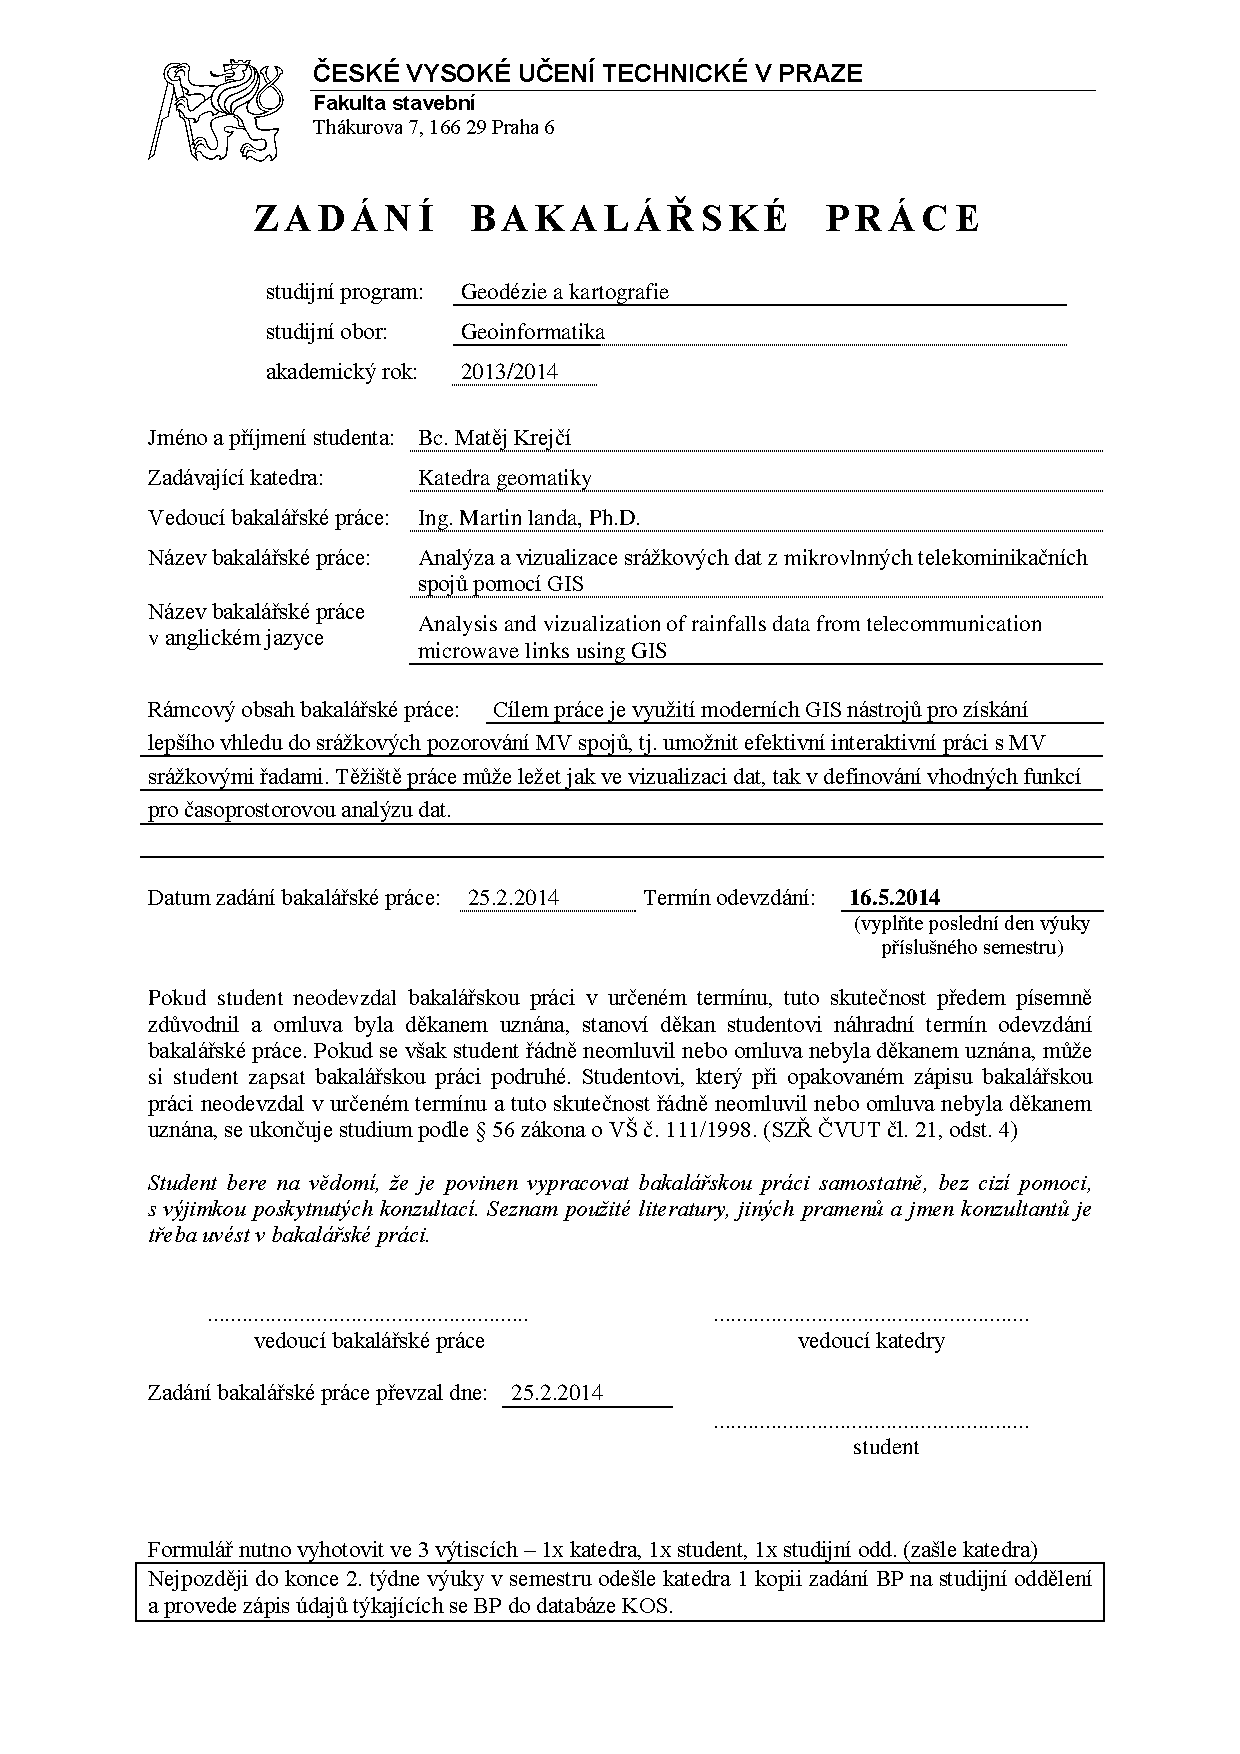
\includepdf[picturecommand={\put(100,200){\vlozZadani}}]{../formulare/zadanibp}
 % resi si zalomeni sam


\begin{abstractpage}
\begin{abstractx}{czech}

  Cílem bakalářské práce je analýza modelování dešťových srážek z dat
  mikrovlnných spojů telekomunikačních operátorů pomocí GIS. Pro
  konkrétní řešení byl použit open source nástroj GRASS GIS. Data ke
  zpracování byla uložena v objektově-relační databázi PostgreSQL. K
  vývoji samotného nástroje byla použita knihovna \textit{GRASS Python
    Scripting Library}. Tento nástroj implementuje rekonstrukci
  dešťových srážek na základě uživatelské konfigurace. Další jeho
  funkcionalitou je příprava srážkových dat plošné reprezentace pro
  časoprostorové analýzy. Hlavní přínos nástroje spočívá v procesu
  primárního zpracování dat pro následné analýzy v hydrologii a
  meteorologii s využitím GIS.


  \klicslova{Klíčová slova}{GIS, GRASS, Python, PostgreSQL,
    dešťové srážky, \newline časoprostorová analýza}
\end{abstractx}

\begin{abstractx}{english}

  The aim of the thesis is modelling of the rainfall data from
  microwave links served by telecommunication operators using GIS. In
  this thesis, well-known open source GRASS GIS is used as a
  framework. The data to be processed are stored in the
  object-relational PostgreSQL database. The GRASS Python Scripting
  Library was used for the GRASS module development. Based on user
  configuration, the module provides the rainfall data
  reconstruction. The geospatial data preparation to be used in
  subsequent spatio-temporal analysis in framework of the temporal
  GRASS system becomes an additional functionality of the developed
  module. Thus, the primary data pre-processing for later analysis of
  hydrological and meteorological processes using GIS tools is
  considered as a main task of the thesis.

  \klicslova{Keywords}{GIS, GRASS, Python, PostgreSQL,
    precipitation, spatio-temporal analysis}
\end{abstractx}
\end{abstractpage}




\newpage
\newcommand{\odsaditodzhora}{\hskip1pt\vfill}

\odsaditodzhora
\noindent Prohlášení
%%% MK: predelano po revizi
Prohlašuji, že bakalářskou práci na téma „Analýza a vizualizace srážkových dat z mikrovlnných telekomunikačních spojů pomocí GIS“ jsem vypracoval samostatně. Veškerá použitá literatura je uvedena v seznamu zdrojů.

\begin{flushleft}
\begin{tabular}{cp{0.3\textwidth}c}
V Praze dne .................
& 
&
..................................
\\
&&
(podpis autora)
\end{tabular}

\end{flushleft}
\newpage

\odsaditodzhora
\noindent Poděkování

Tady bude podekovani

\newpage

\newpage

\tableofcontents


\newpage
\necislovana{Úvod}

\pagestyle{fancy}
\fancyhf{}
\renewcommand{\sectionmark}[1]{\markboth{#1}{}} % set the \leftmark
\fancyhead[L]{ČVUT v Praze}
\fancyhead[R]{\leftmark} % 1. sectionname
\fancyfoot[C]{\thepage}


\pagenumbering{arabic}
\setcounter{page}{1}
\subsection*{Předmluva}

%%% ML: text a hlavne zavery z neho plynouci jsi z neceho cerpal
%%% (predpokladam), potom chybi ale citaci, ty zavery je potreba o
%%% neco oprit
%%% MK: citace doplneny, prvni odstavec je z vlastnich poznatku. 
%%% Celkove uvod je hodne z vlastnich poznatku ziskanych v ramci bp.
%%% (vseobecnej prehled). Muze to tak byt?
%%% ML: OK (jenom jsem odstranil carky pred citaci)

Enviromentální procesy jsou nedílnou součástí historického vývoje na
Zemi a~vždy přitahovaly pozornost lidské populace. Obvykle jsou tyto
jevy komplexního charakteru a pro jejich pochopení je nutné
interdisciplinárních přístupů. S vývojem informačních technologií jsou
dostupné ke studiu problematik stále propracovanější metody, které
umožňují komplexnější přístup a pochopení dějů v širším kontextu. Mezi
tyto metody se bezesporu řadí numerické fyzikálně založené modely, kterých by
bez výpočetního výkonu nebylo možno využít. Informační technologie v
současné době dosahují velkého rozvoje a rozšíření i díky stále
rostoucí výpočetní výkonnosti. Tato skutečnost umožňuje využívat
metod, které by ještě do nedávna nebylo možné aplikovat.

Většina modelů, které simulují přírodní procesy, jsou pro jejich
komplexnost charakteristické značnými objemy dat, které je nutné
spravovat a analyzovat. V~posle\-dních desetiletích tuto práci výrazně
usnadňují nástroje geografických informačních systémů (GIS),
které díky své dostupnosti a možnostem nacházejí nezastupitelné místo
ve správě a analýze geografických dat \cite{coppock}.
Jednotlivé nástroje GIS zpravidla nebývají
úzce zaměřené na specifické problematiky, ale jejich spíše obecný
charakter umožňuje návaznost a možné propojení s vlastními aplikacemi.
Tím ulehčuje vytvoření nástrojů pro řešení komplexních systémů.

\subsection*{Motivace}

%%% ML: bez citaci, viz predchozi odstavec
%%% ML: OK
Modelování dešťových srážek je jednou z významných disciplín z oboru
enviromentálního modelování. Jestliže se poohlédneme do 
minulého století, tak právě meteorologie byla jednou z prvních
disciplín, která by ze současného pohledu odpovídala pojmu enviromentálního
modelování \cite{wpc, neuman}. Odhad a rekonstrukce srážek na 
zemském povrchu jsou důležitou fází matematického modelování srážko-odtokových
procesů. Zájem odborné veřejnosti i rozhodovacích složek v různých
sektorech národního hospodářství roste i díky stále hlouběji se
projevujícímu dopadu klimatických změn. Oproti rozvoji fyzikálně
numerických modelů nebyl technologický pokrok ve sběru srážkových dat
v posledních desetiletích takřka zaznamenán. Pracovníci
hydrometeorologických služeb naráží při zpřesňování předpovědí odtoku
či vývoje počasí především na problém nízkého pokrytí srážkoměry a tím
i nedostatečné dostupnosti časoprostorového rozložení srážkových dat v
povodněmi ohrožených oblastí městských aglomerací \cite{slavicek}. Pokrokové
%%% ML: pouzivat zkratka MV, ale nevysvetlena
%%% ML: OK
operativní metody určování srážek metodou MV (mikrovlnných) spojů proto představují
perspektivní využití především v hydrologii urbanizovaných povodí, kde
díky hustotě MV sítí mohou sloužit jako podklad vodohospodářských
dispečinků operativního řízení při řešení kalamitních povo\-dňových
situací \cite{countryw}.



\subsection*{Cíl}
Hlavním cílem práce je vývoj nástroje pro zpracování hrubých dat
z MV vysílačů v prostředí GIS a současně jejich zpřístupnění pro 
další analýzy, které
pomohou zefektivnit výzkum těchto nových metod. Svým vedlejším
výstupem je práce zaměřena na využití výstupů z GIS
pro interpretaci plošných srážek. V návaznosti na vývoj nástroje pro
zpracování hrubých dat z MV spojů je demonstrováno využití
časo\-prostorových analýz v GIS.

Téma práce vychází z požadavků zpracovatele projektu, který se zabývá
problematikou odhadu srážek z MV spojů v rámci projektu
"TeleMAS"\footnote{GA ČR 14-22978S \uv{Predikce srážkového odtoku v
  urbanizovaných povodích na základě deštěm generovaného útlumu
  signálu mikrovlnných spojů telekomunikační sítě}} v souvislosti s
modelováním srážko-odtokových procesů v městských povodích. Tento
projekt je řešen v úzké vědecké spolupráci s ETH\footnote{
  Eidgenössische Technische Hochschule
  Zürich}-EAWAH\footnote{Eidgenössische Anstalt für Wasserversorgung,
  Abwasserreinigung und Gewässerschutz} a odborné spolupráci se
společnostmi T-Mobile a Veolia ČR a nově i s Ericsson Research
(Sweden).

Práce je systematicky rozdělena na část teoretickou a praktickou. V
teoretické části je kladen důraz na představení základních pojmů,
principů a definic, tvořících východiska pro část praktickou. Ta
obsahuje popis funkčnosti nástrojů, které vznikly v rámci této práce a
 jejich využití ve spojení s ostatními GIS nástroji.

 



\newpage
\chapter*{Teoretická
  část}\stepcounter{chapter}\addcontentsline{toc}{chapter}{Teoretická
  část}

Tato kapitola je základním teoretickým východiskem k praktické části
práce dotýkající se problematiky MV spojů a použitých technologií pro
vývoj vlastních GIS nástrojů.
%%% ML: tato veta (viz nize) zni divne, uplne bych ji vynechal...
%%% MK: smazano
%%% ML: OK

%%% ML: efektivne "mamagement", preformuluj to tak, aby to znelo vice
%%% cesky
%%% MK: spojeni dvou vet do jedne
%%% ML: OK
\paragraph*{Geografické informační systémy} mimo jiné umožňují poměrně
efektivně  správu, analýzu a vizualizaci sráž\-kových dat. 
Jednotlivé metody měření srážek jsou specifické svojí
datovou charakteristikou jak z prostorového tak časového pohledu.

Metody měření srážek ze své podstaty využití směřují ke kombinaci
plošné a bodové informace, které jsou svoji charakteristikou
rozdílné. Srážkoměry produkují bodová data v různých časových
intervalech. Naopak výstupem z radaru či meteorologických družic jsou
snímky představující plošnou
%%% ML: satelitni druzice zni divne...
%%% MK: predelano
%%% ML: tu vetu jsem zjednodusil, zkontroluj to...
intenzitu srážek. 
%%% ML: jake druhy dat? 
%%% MK: predelano
Společné je pro tyto metody potřeba výstupy co nejjednodušeji
spravovat a analyzovat, jak v rámci primárního tak sekundá\-rního
zpracování. Primární zpracování hrubých měřených dat spočívá v jejich převodu
do formy, která umožní analýzy v prostředí GIS, tj.~sekundárního
zpracování.
%%% ML: pojmy primarni a sekundarni zpracovani nejsou vysvetleny
%%% MK: vysvetleno
%%% ML: OK, i kdyz mi to zni porad divne, ale OK (trosku jsem to preformuloval, radeji to zkontroluj)
GIS nástroje splňují tyto
požadavky v dostatečném rozsahu a~částečně eliminují potřebu vývoje
specifických solitérních systémů, které by vychá\-zely ze stejných
základů.

Charakteristikou moderních GIS je především velká disponibilita
dílčích funkcí, jejichž hlavní přínos spočívá v možnosti vzájemného
propojení v rámci rozsáhlých analýz. Pokud dostupné funkce konkrétního
GIS nástroje k řešení daných problematik nedostačují, bývá obecně u
většiny těchto systémů možnost vývoje vlastních aplikací postavených
na knihovnách GIS. Díky tomu je v dnešní době umožněno vyvíjet
specifické funkce pro GIS, bez nutnosti vývoje rozsáhlých softwarových
produktů vytvářejících základy pro tato nadstavbová rozšíření.



\section{Úvod do měření dešťových srážek}
Úvod této kapitoly má za cíl přiblížit současné metody měření dešťových
srážek, které se liší především v přesnosti, časové variabilitě a
vhodnosti výstupu pro další využití. Úvod do problematiky měření
srážek poukazuje na klady a zápory metody odhadu srážek pomocí MV spojů.


\paragraph*{Dešťové srážky} jsou definovány jako produkt vodní páry v
kapalném nebo pevném stavu, které padají z oblohy či se kondenzují přímo
na zemském povrchu. Srážky mohou mít formu sněhových vloček - pevné
skupenství nebo formu dešťových kapek - kapalné skupenství. Množství
srážek bývá udáváno v milimetrech kapalné vody spadlé na zemský povrch
za časový interval \cite{wmo}.

\subsection{Současné nástroje a metody }
\label{subsec:11}

\subsubsection{Srážkoměry}
Srážkoměr je přístroj používaný v meteorologii a hydrologii k měření
srážkových úhrnů. Dle funkčnosti se srážkoměry dělí na dešťové a na
srážkoměry, které měří i srážky pevného skupenství. Tyto srážky se
přeměňují na ekvivalent vody a až poté vyhodnocují. Důležité je
podotknout, že produktem srážkoměrů jsou bodová srážkoměrná data.

\subsubsection{Meteorologický radar}
Radarová měření díky plošnému pokrytí a dobrému prostorovému i
časovému rozlišení dat jsou vhodná pro synoptickou a leteckou
meteorologii. Poskytují přehled v~reálném čase o pohybu a struktuře
srážkových systémů, umožňují velmi krátko\-dobou předpověď v řádech
minut až hodin a z ní plynoucí varování před nebezpečný\-mi
meteorologickými jevy \cite{radar_chmu}.

\paragraph*{Srážková data} se měří obvykle v intervalu 5 -15
minut. Horizontální rozlišení dat bývá 2×2 km, vertikální 1 km. Toto
prostorové rozlišení je nutné, aby bylo možné zachytit jednotlivá
srážková jádra přeháněk. Radarové odrazy jsou interpretovány plošně a
jsou zobrazovány v barevné stupnici intenzit srážek.

\paragraph*{Rozsah} meteorologického radaru bývá okolo 250 km. Hodnoty
naměřené radarem mohou být použity pro odhad okamžitých intenzit
srážek do vzdálenosti přibližně 150 km od radaru \cite{kohout}.

\subsubsection{Dálkový průzkum Země}
Je důležité zmínit možnost získávání informací o srážkách pomocí
  \acs{DPZ}. Tento obor z hlediska meteorologie zaujímá zcela jiný
náhled na měření srážek oproti předchozím metodám. \acs{DPZ} v
meteorologii umožňuje globální pohled na meteorologické jevy. Makro
náhled na enviromentální jevy, např. cyklóny, tropické bouře, tornáda
či pohyb mraků, je podstatný pro sledování a pochopení globálního
vývoje klimatu. Do této kategorie spadá pozorování pomocí družic na
oběžných drahách a~leteckých prostředků pohybujících se v zemské
atmosféře.


\subsection{Mikrovlnné spoje}
\label{subsec:}
%%% ML: Zkratku ML pouzivas uz mnohem drive v textu
%%% MK: pravda
%%% ML: pridal jsem zkratku do zavorek (MV)
Mikrovlnné spoje (MV) jsou rádiové systémy široce využívané v oblasti
telekomunikací (zejména mobilními operátory) k bezdrátovému propojení
dvou vzdálených stanovišť. MV spoje operují na frekvencích, kde
dešťové kapky představují hlavní zdroj útlumu signálu. Analýza útlumu
signálu umožňuje poměrně přesně odhadnout průměrnou srážkovou
intenzitu podél spoje. Vzhledem k hustotě sítě MV spojů (např. v Praze
řádově stovky až tisíce) jde o relevantní zdroj srážkové informace,
který má velký potenciál zlepšit prostorovou informaci o srážkových
intenzitách. Využití standardních GIS nástrojů může výrazně
zefektivnit jak zpracování dat, tak jejich následnou správu.  Vhodná
vizualizace těchto dat je důležitým předpokladem pro vylepšení
stávajících modelů pro převod útlumu signálu MV spojů na srážkové
intenzity i pro další využití těchto dat.

\newpage %%% ML: kvuli poznamce pod carou, pri zmene strankovani nutno opravit
		 %%% MK: diky
%%% ML: uz tu zadnou poznamku pod carou nevidim, ale strankovani je OK
\begin{figure}[h!]
    \centering
    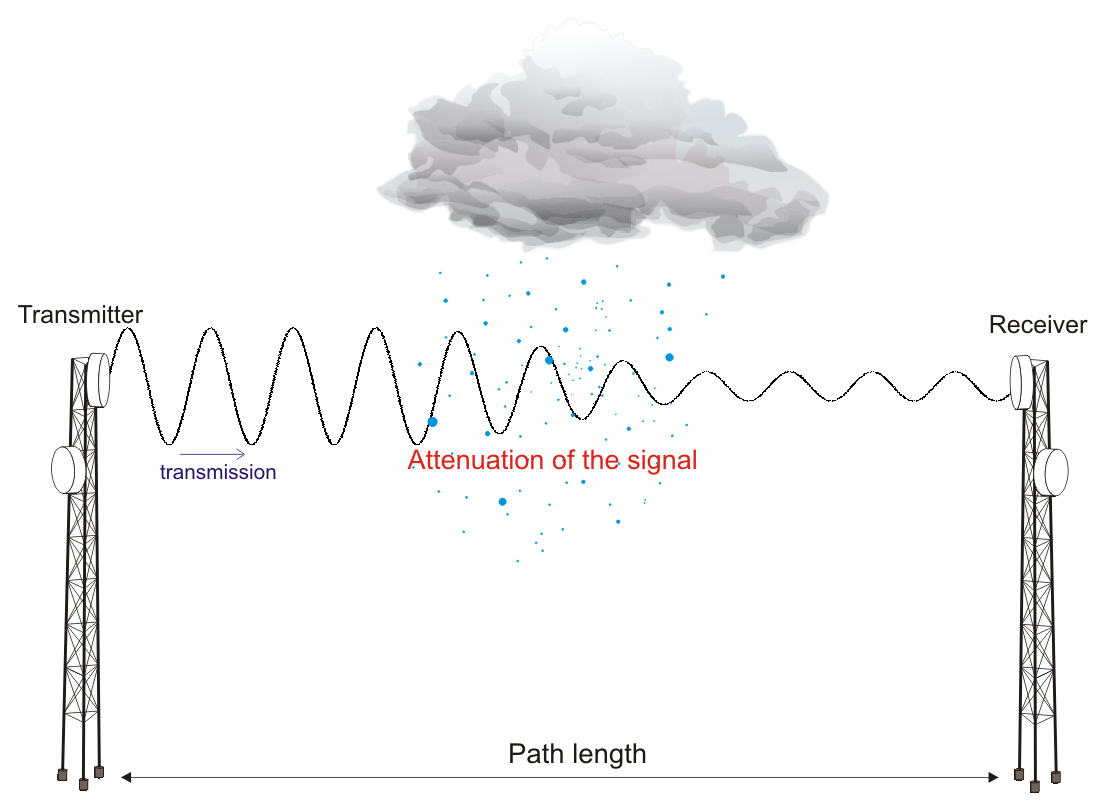
\includegraphics[width=0.7\textwidth]{./img/srazky/microwave_link.png}
    \caption[Rušení radaru]{\centering Útlum intenzity mikrovln způsobený srážkami\footnotemark}
 \end{figure}   
  \footnotetext{\url{http://lte.epfl.ch/page-50160-en.html}}

\subsubsection{Data}
Charakteristika dat z MV spojů je zcela unikátní v oblasti měření
srážek. Specifická je především reprezentací hodnoty srážkové
intenzity v liniové podobě. MV spoje (linie), umožňují odhadovat pouze
průměrnou intenzitu srážky v celé délce spoje a z toho plynou jisté
meze této metody. Na hustě osídlených územích bývá pravidlem, že i
hustota MV spojů je veliká. V tomto případě je tento zápor částečně
potlačen (Evropa). Oproti tomu, při využití MV spojů mimo osídlené
lokality, je hustota poněkud menší a to limituje možnosti
využití. Příkladem může být transformace srážek do povodí: uvažme
např.  spoj, který vede kolmo přes cílovou lokalitu. V případě že
lokalita zasahuje do desetiny délky spoje, je pravděpodobnost toho, že
srážka spadla právě do lokality velmi nízká a to především díky
variabilitě intenzit srážek. Oproti tomu transformace srážek do
povodí, kde spoj bude ležet v celém území povodí je ideální.

Obecně jsou data z MV spojů měřeny v časovém kroku $\Delta t=15$ s,
ve výšce cca 70~m. Topologie sítě představuje vždy jeden
referenční vysílač, na který jsou napojeny dílčí vysílače. Na jednom
spoji jsou instalované zpravidla dvě antény. Je tedy k dispozici
dvoje měření pro stejný prostorový úsek. V ideálním případě jsou dvě
antény na stejném prostorovém úseku různých konfigurací (frekvence,
polarizace), což umožňuje specifické analýzy.

    
\subsubsection{Princip metody}

Mikrovlny jsou elektromagnetické vlny o délce v rozpětí od 1 mm do 1
m. Tomu odpovídá frekvence 0.3 až 300 GHz. V oblasti
telekomunikací především mobilních operátorů se tohoto typu vln
využívá ke komunikaci mezi jednotlivými vysílači a~vysílači s
mobilními telefony. Pro rekonstrukci srážek se využívá prvního
případu, tedy komunikaci mezi vysílači. Tyto mikrovlnné spoje pracují
na frekvencích v~roz\-sahu 24-39 GHz (Praha). Hlavním zdrojem útlumu
tohoto frekvenčního rozsahu jsou dešťové kapky. Jednotlivé spoje se
vždy skládají ze dvou vysílačů. Vysílač neustále odesílá MV vlny,
které jsou nositelem informace zajímavé především pro telekomunikační
operátory. Vedlejším produktem této komunikace je údaj o intenzitě
signálu, jehož základní jednotkou je decibel (dB). Zaznamenat hodnotu
intenzity odeslaného signálu a druhým přijímačem přijatého signálu je
možné bez dalších instalací hardware. Pomocí matematického
modelu dle ITU-R \cite{itu} lze vypočítat průměrné srážky na pomyslné
linii MV spoje.

\subsubsection{Výpočet srážek}

Vysílané hodnoty intenzit signálu \emph{tx} jednotlivých MV spojů jsou
konstantní. Jednotlivé spoje jsou charakterizovány hodnotami:
\begin{itemize}
\item \textbf{frekvence} \emph{f} rozsahu 24-39 (GHz),
\item \textbf{polarizace} signálu ve vertikální \emph{V} či horizontální poloze \emph{H},
\item \textbf{vzdálenost} \emph{L} která je vypočtená v daném souřadnicovém systému v kilometrech (km).
\end{itemize}
Přijaté hodnoty intenzit \emph{rx} jsou nositelem informace o útlumu
signálu. Rozdílem vyslané \emph{tx} a přijaté \emph{tx} intenzity
dostaneme výsledný útlum \emph{$A_{r}$} v jednotkách decibel (dB).
\begin{equation}
 A_{r}=tx-rx
\end{equation}
Dalším krokem je určení \emph{baseline}, tedy hodnoty \emph{ $A_{0}$},
 která představuje konstantní útlum intenzity signálu MV spoje bez
vlivu útlumu signálu dešťovými kapkami. Tato konstanta je udávána v jednotkách
decibel (dB). Konstanta \emph{$A_{w}$} je hodnota
nadměrného útlumu způsobená mokrou anténou. Z toho plyne výsledný
útlum \emph{$A_{m}$}~(dB).
\begin{equation}\label{eq:Ar}
 A_{m}=A_{r}-A_{0}-A_{w}
\end{equation}
Výsledný útlum je třeba převést na specifický útlum \emph{$\gamma_{R}
  $} ($db \cdot km^{-1}$) pro danou vzdálenost \emph{L} mezi vysílači MV spojů.
\begin{equation}
\gamma_{R} =\frac{A_{m}}{L}
\end{equation}
Dle doporučení ITU P.838 \cite{itu} je specifický útlum
\emph{$\gamma_{R} $} a intenzita srážek \emph{R} ($mm \cdot h^{-1}$) ve vztahu
\begin{equation}\label{eq:gamma}
\gamma_{R}=kR^{\alpha}
\end{equation}
Koeficienty \emph{k} a \emph{$\alpha$} jsou určeny jako funkce
frekvencí \emph{f} v rozsahu od 1 do 1000 GHz, z následujících rovnic.

\begin{equation}
log_{10}k=\sum_{j=1}^{4} a_{j} exp\left [ -\left ( \frac{log_{10}f-b_{j}}{c_{j}} \right )^{2} \right ]+m {_{k}}log_{10}f+c_{k}
\end{equation}

\begin{equation}
\alpha=\sum_{j=1}^{5} a_{j} exp\left [ -\left ( \frac{log_{10}f-b_{j}}{c_{j}} \right )^{2} \right ]+m{_{\alpha }}log_{10}f+c_{\alpha }
\end{equation} 
kde:

\emph{f}: frekvence (GHz),

\emph{$\alpha$}:  dle polarizace \emph{$\alpha_{H}$} nebo \emph{$\alpha_{V}$},

\emph{k}: dle polarizace  \emph{$k_{H}$} nebo \emph{$k_{V}$}.

{\raggedright{}Hodnoty pro  konstanty  $c_{k}$, $c_{\alpha}$, $m_{k}$, $m_{\alpha }$  jsou uvedeny v dokumentu 
  ITU-R \cite{itu}.}  \bigskip

{\raggedright{}  Z rovnice \eqref{eq:gamma} dostaneme
  výslednou intenzitu srážek \emph{R} ($mm \cdot h^{-1}$). }


\begin{equation}
R=\left ( \frac{\gamma_{r}}{k} \right )^{\frac{1}{\alpha }}
\end{equation}


\subsubsection{Chyby}
\label{subsec:chyby}
Metoda odhadu srážek je založena na předpokladu, že dešťové kapky
tlumí intenzitu signálu. Dešťové kapky nabývají mnoha variací
velikosti a tvarů. Signál může být tlumen různými objekty počínaje vodní
párou, přes mrholení až po velké dešťové
kapky či srážky pevného skupenství. Vztah mezi intenzitou srážek \emph{R} a~útlumem
\emph{$\gamma_{R} $} je funkcí frekvence, polarizace a rozložení
dešťových kapek   \acs{DSD}.

Na frekvencích mezi 25 a 40 GHz platí takřka lineární závislost a
model je téměř nezávislý na teplotě, rozložení dešťových kapek a
empiricky vykazuje chyby méně než 10\emph{\%}. Na nízkých
frekvencích okolo 10 GHz přesahuje chyby 20\emph{\%}. Přesnost
určování srážek výše zmíněným modelem dle ITU P.838 je při těchto
nízkých frekvencích mnohem více náchylná na rozložení
kapek   \acs{DSD} \cite{dsd}.

\paragraph*{Určení baseline} \emph{$A_{0}$} je jedním z důležitých
a nejvíce ovlivňujících činitelů při výpočtu výsledné srážky
\emph{R}. Jde o pozaďovou (referenční) úroveň signálu, vůči které je 
posuzován útlum signálu - veličina nutná k odhadu srážek. Za pozaďovou 
hodnotu je považována úroveň signálu během suchého období, která 
ovšem může kolísat. Proměna \textit{baseline} v čase a je závislá na
%%% ML: pojem scintilace by mozna bylo vhodne vysvetlit (napr. poznamka pod carou)
%%% MK: vysvetleno 
%%% ML: OK
koncentraci vodní páry v atmosféře a scintilaci 
\footnote{Scintilace je jev, při kterém vznikají slabé světelné záblesky (pulsy světla) v některých 
látkách při dopadu ionizujícího záření.}. Útlum vysílaných a
přijímaných vln ovlivňuje také teplota prostředí, jímž vlna
prochází. Dalším činitelem, který může způsobovat kolísání signálu, je
vítr.  Pro určování baseline se využívá různých metod, například
   \acs{HMM} \cite{comparsinmv}, Retrieval Algorithms
\cite{countryw} atd. Metody určení baseline se dají klasifikovat na
automatizované a uživatelské. Automatizovaným určováním baseline se
myslí především algoritmy, které jsou schopny rozlišovat dešťové a suché
období. Některé tyto algoritmy využívají statistických prostředků a
jiné např. určují období srážek pomocí dat ze srážkoměrů
\cite{countryw} či radaru.


\paragraph*{Nejistoty modelu} založeného na vztahu \eqref{eq:Ar} jsou
především v závislosti \emph{$\gamma_{A_{m}} $}, \emph{$A_{w} $} na
rozložení kapek   \acs{DSD} podél MV spoje.

\paragraph*{DSD} způsobují nejistoty při určení výsledného útlumu
signálu \emph{$\gamma_{A_{m}} $}. Tyto chyby jsou zapříčiněny
integrací jednotlivých úseků tlumících signál na linii MV
spoje \cite{mv1}.

\paragraph*{Mokré antény} jsou značným zdrojem nejistot. Na vysílačích
nejsou antény nijak kryty a při dešti moknou. Na anténách se vytváří
tenký film vody, který ovlivňuje výsledný útlum signálu. Vytvoření
modelu pro eliminaci tohoto problému se do značné míry podařilo
(Schleiss et al., 2013) \cite{wetat}. Součástí výzkumu, pod který tato
práce částečně spadá, bude instalace krytu na antény, který by mohl
zamezit jejich moknutí. Tato možnost doposud nebyla součástí žádné
vědecké práce.



\subsection{Porovnání metod}
Tato podkapitola je zaměřena na shrnutí vlastností jednotlivých metod
a jejich porovnání s metodou MV spojů. Hodnocení jednotlivých metod je
založeno na kritériích, která jsou pro měření srážek typická:
\begin{itemize}
\item\textbf{časová spojitost},
\item\textbf{interval sběru dat},
\item\textbf{prostorové rozlišení},
\item\textbf{disponibilita jednotlivých metod},
\item\textbf{chyby}.
\end{itemize}
V současné době jsou v oblasti hydrometeorologie požadována velmi
přesná data ve vysokém prostorovém a časovém rozlišení. Tyto nároky
jsou především vytvořeny požadavky hydrologických modelů, jejichž
výsledky napomáhají k lepšímu operativnímu řízení odtoku v
urbanizovaných územích. Kvalita vstupů dat do těchto modelů je
rozhodující pro jejich přesné výsledky, které jsou základem
návrhu protipovodňových opatření.

\paragraph*{Srážkoměrné sítě} 
tyto požadavky splňují jen částečně. Moderní srážkoměry splňují
kritérium schopnosti vytvoření spojité časové řady až v minutových
intervalech. Hlavním záporem těchto sítí je nedostatečné prostorové pokrytí. 
Jelikož datovým výstupem těchto sítí jsou bodová data, je zde
problém v nedostatečné hustotě pokrytí srážkoměry, která prakticky
nemůže být nikdy odstraněna. Prostorová variabilita  srážek
 má za následek zachycení či naopak nezaznamenání lokálních maxim, které jsou ve
výsledné plošné rekonstrukci zdrojem nezanedbatelných chyb. Měření
moderními srážkoměry může být při správné volbě umístění velmi
přesné. Toho se v současnosti využívá jako referenčního indikátoru
srážek pro kalibraci radarů nebo k určování baseline při odhadu
srážek MV spoji, viz kap. \ref{subsec:chyby}.

\paragraph*{Radary}
jsou současnou nejvíce využívanou metodou, jejímž produktem je plošné vyjádření srážek.
Skutečnost, že se intenzity srážek mohou během intervalu 
pozorování (5-15 min) řádově měnit, naznačuje nespolehlivost jejich předpovědi 
v~pří\-padě bleskových povodní. Mezi kladné vlastnosti radaru
bezesporu patří mimo klasické rozlišení v horizontálním směru (plošné)
také měření odrazivosti vertikálních profilů. Tuto vlastnost v
rozlišení 1 km pro vertikální a 2 km pro horizontální směr ostatní metody
neumožňují. Prostorové rozlišení je dále možno pozorovat jen pomocí
některých meteorologických družic, které snímají povrch Země pod sklonem
jiným než 90 stupňů. Jejich rozlišení je ale v desítkách jednotek
horší. Pro zpřesnění radarových srážek pro potřeby hydrologie je
potřeba adjustace radarů na pozemní srážkoměry. Obecně vzato je
výsledné plošné rozlišení radaru pro srážko-odtokové modely
 ve městech nedostačující.

\paragraph*{Družice} se s výše zmíněnými metodami nedají zcela
korektně porovnávat. Družice na oběžných drahách slouží především k
náhledu na chování klimatu. Snímky pořízené z těchto družic jsou nositelem
informací v rozlišení, reflektující spíše obecnou informativní
podstatu, např. pohybu front, vývoje cyklónu, globální přehled vývoje
počasí či dlouhodobě - klimatu.  Jednou z výhod rekonstrukce srážek
pomocí metody infračerveného pásma je poměrně vysoká frekvence záznamu
snímků v intervalu 15 minut na jakémkoliv místě na Zemi. Při porovnání
s pozemním meteo radarem je slabost této metody ve špatném a u
některých družic nulovém detekování vertikálních profilů srážkových
mraků, což vede k podceňování výsledných srážkových úhrnů.


\subsubsection{Mikrovlnné spoje}
Metoda odhadu srážek pomocí MV spojů byla předmětem výzkumu už v
80. letech 20. století. Prakticky byla použita až při využití
komerčních telekomunikačních spojů v posledním desetiletí. Budoucnost
této metody je také v pokrytí osídlených oblastí, kde je právě
přesnost odhadu srážek nejvíce vyžadována. Pokrytí s vývojem mobilních
technologií se stále zlepšuje. Data jsou sbírána ve velmi malých
intervalech běžně po 15 sekundách. Při využití rozsáhlých sítí (Praha - stovky
MV spojů), umožňuje tato metoda relevantní časoprostorovou informaci o
srážce.
 
\paragraph*{Potenciál MV v hydrometeorologii} zasahuje do všech
oblastí vědních oborů, kde se využívají srážky jakožto vstupní časové
řady. Tato metoda je v současné době spíše vhodná pro lokální využití
nežli regionální. Vyplývá to z absence pokrytí sítí mimo osídlené
oblasti.
 \begin{figure}[h!]
    \centering
    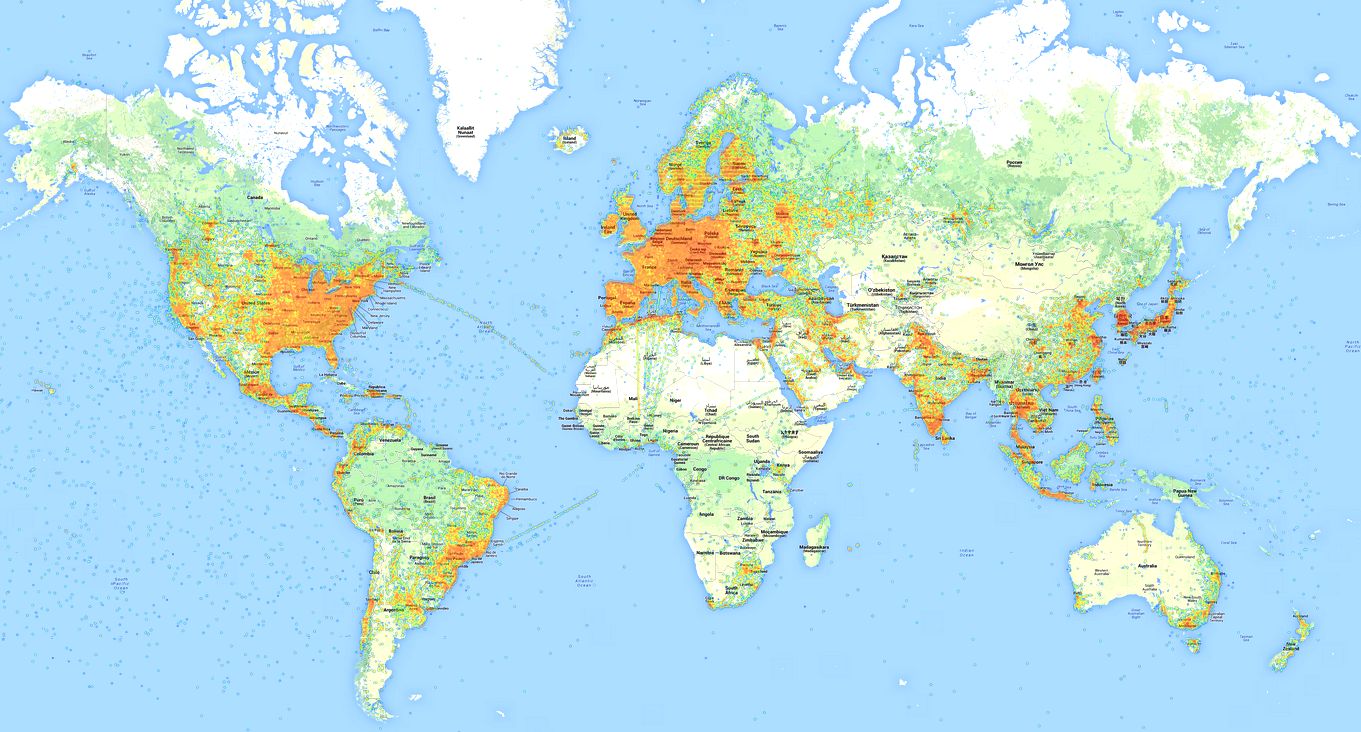
\includegraphics[width=1\textwidth]{./img/srazky/opensignalmap.png}
    \caption[Porytí tel. sítí]{\centering Mapa celosvětového pokrytí signálu telekomunikačních mobilních operátorů. Pokrytí je vyjádřeno oranžovou a žlutou barvou. \footnotemark }
    \label{fig:pokryti}
 \end{figure}   

Jedním z velkých potenciálů této metody je zlepšení přesnosti
prostorové informace o srážkách ve vysokém rozlišení. To žádné jiné
metody odhadu srážek neumožňují. Výsledky studie \cite{mv2} poukazují na
možnosti částečného nahrazení současných metod nebo možnosti
vzájemného se doplňování jednotlivých metod, což by patrně vedlo k
zlepšení přesnosti měření srážek.

Jelikož tyto MV spoje operují těsně nad zemským povrchem, vypočtené
intenzity by mohly být pomocí nástrojů \acs{GIS} velkou přesností
přiřazovány do jednotlivých dílčích povodí. To by zpřesnilo vstupy do
srážko-odtokového modelu a umožnilo lépe modelovat členitá povodí ve velkých městských aglomerací.

Možnosti využití MV spojů v oblasti meteorologie nekončí u odhadu
srážek. Pomocí MV lze také detekovat pevné částice, sníh či vodní
páry. Tyto možnosti by mohly napomoci k lepšímu pochopení jevů
spojených s přívalovými srážkami \cite{mv2}.


Velkým potenciálem je takřka nulová finanční náročnost pro sběr
dat. Telekomunikační sítě mobilních operátorů jsou v hustěji
osídlených částech světa běžné.\ref{fig:pokryti} V~rychle se rozvíjejících zemích
třetího světa se v průběhu času stanou telekomunikační sítě
samozřejmostí a využití metody odhadu srážek pomocí MV spojů by se mohlo stát více
dostupnou oproti budování radarů, pozemních stanic či sítě
srážkoměrů.
\footnotetext{Obrázek byl sejmut z webové aplikace OpenSignal. \url{http://opensignal.com/}}

\setcounter{footnote}{1}



\newpage
\setcounter{footnote}{1}
\section{Použité technologie}

\subsection{Systém GRASS GIS}
\textbf{GRASS} (Geographic Resources Analysis Support System) GIS
\footnote{\url{http://grass.osgeo.org/}} je multiplatformní
geografický systém, šiřitelný pod všeobecně veřejnou licencí \acs{GNU
  GPL}. Systém je primárně určený pro správu 2D/3D rastrových a
vektorových geodat, jejich zpracování, analýzu a vizualizaci. K těmto
účelům systém GRASS GIS disponuje několika stovkami nástrojů,
tzv. \uv{modulů}.  Mimo to je volně dostupných mnoho dalších modulů,
které jsou vyvíjeny uživateli v rámci GRASS \textit{AddOns}.
%%% ML: tohle bych klidne vynechal
% a~mohou se
%stát součástí stabilních vývojových verzí GRASS.
%%% MK: ok

GRASS GIS je na poli GIS software zcela unikátní a to především díky
%%% ML: pravda je, ze velka cast kodu pochazi z USA CERL, ktery system
%%% vyvijel do poloviny 90.let..., OK zminujes to dal v textu, tedy OK
svému rozsahu, čemuž vděčí především dobrovolným vývojářům z komunity
GRASS po celém světě, kteří tento dlouholetý projekt vyvíjí. Důkazem jeho
kvality jsou uživatelé jako např.
%%% ML: tady bych odkazy klidne vynechal, prilis mnoho poznamek pod carou,...
%%% MK: ok
\textit{NOAA} či %\footnote{\url{http://www.noaa.gov/}}
\textit{NASA}.%\footnote{\url{http://www.nasa.gov/}}.

\begin{figure}[h!]
    \centering
    
\includegraphics[width=0.3\textwidth]{./img/grass/grasslogo.png}
    \caption[Logo GRASS]{\centering Logo GRASS GIS vydané symbolicky k 30. výročí od založení projektu \footnotemark. }
 \end{figure}   
\footnotetext{Autorka úpravy oficiálního loga: Žofije Marcela Zetková, \url{http://grass.osgeo.org/uploads/images/30-years-grass-gis-logo-black-300px.png}}


\subsubsection*{Historie}
%%% ML: moc nerozumim slovu "stala" v teto souvislosti...
%%% MK: predelano
%%% ML: preformulovano, klidne zmen
Vývoj GRASS GIS sahá do poloviny osmdesátých let minulého
století. Tehdy byl vyvíjen primárně pro americkou armádu, která jej
využívala pro územní správu a plánování. Během 90. let se postupně na
vývoji projektu podíleli americké federální agentury, univerzity a
soukromé společnosti. Hlavní vývoj projektu byl řízen z výzkumných
laboratoří (USA-CERL\footnote{\url{http://www.cecer.army.mil/}})
Champaign, Illinois \cite{grasshist}.  Mezníkem historie systému GRASS byl
rok 1995, ve kterém se laboratoře CERL zřekli tohoto projektu, čehož
následkem bylo přesun vývoje na akademickou půdu. Rok před začátkem
nového tisíciletí byla vydána první verze pod licencí GNU GPL, pod
kterou je vyvíjen dodnes. V letech 2008 se GRASS GIS zařadil pod hlavičku nadace
   \acs{OSGeo}, pod kterou spadá mnoho významných volně šiřitelných
GIS
projektů \footnote{\url{http://www.osgeo.org/}}. Letošním rokem
oslavil GRASS dlouhých 30 let vývoje.
%%% Minuly rok v cervenci byla vydana verze 6.4.3
%%% MK: smazano
%%% ML: OK
\subsubsection*{Základní terminologické pojmy}
\label{subsubsec:grassterminologie}
Hlavním cílem této sekce je představit základní filosofii
uživatelského rozhraní systému GRASS GIS.
\paragraph*{Data} ke kterým GRASS přistupuje, jsou definována pevně
stanovenou adresářovou strukturou. Pro práci v tomto systému, je prvně
zapotřebí definovat trojici nastavení. V grafickém rozhraní GRASS
   \acs{wxGUI} je implementován průvodce nastavením jednotlivých kroků:

\begin{enumerate}
\item \textbf{Databanka} v prostředí GRASS je stanovena proměnou
  \texttt{\$GISBASE}. Jedná se o standardní adresář umístěný na disku.
%%% ML: adresar se muze jmenovat jakkoliv
%  který je pojmenován \textit{grassdata}.
%%% MK: to je fakt...
  V tomto adresáři jsou uložena veškerá uživatelská data s vyjímkou
  externě připojených databází (\textit{např. PostgreSQL, MySQL}).

\item \textbf{Lokace} je adresář umístěný v souborové
  databance. Lokace je definována proměnou \texttt{\$LOCATION\_NAME} a
  obsahuje data, která nesou informace o souřadni\-covém systému a
  velikosti zájmového území. Pro nastavení lokace je v grafickém
  rozhraní průvodce nastavením lokace (\textit{Location wizard}), kde
  je možné zvolit souřadnicový systém na základě několika možností:
%%% ML: pozor na termin "projekce" v cestine neznamena to co v anglictine
\begin{itemize}
\item seznam jednotlivých obecně známých kartografických zobrazení, 
\item zadáním unikátního kódu z databáze    \acs{EPSG}. \footnote{\url{http://www.epsg-registry.org/}},
\item načtením externích georeferencovaných dat,
\item definováním parametrů souřadnicového systému s využitím pravidel\newline PROJ.4\footnote{\url{http://trac.osgeo.org/proj/}},
\item pomocí \ac{WKT}\footnote{WKT je značkovací jazyk pro reprezentaci vektorových objektů na digitálních mapách.} souboru \emph{.prj}, který je součástí formátu Esri Shapefile.
\end{itemize}

\item \textbf{Mapset} definovaný proměnou \texttt{\$MAPSET}
  představují jakýsi profil uživatele, či profil ucelených analýz v
  dané lokaci. Každá lokace musí obsahovat mapset, který má unikátní
  název \texttt{PERMANENT}. Do tohoto mapsetu se z pravidla ukládají
  vstupní data, ke kterým se z ostatních pracovních mapsetů
  přistupuje.
\end{enumerate}



\paragraph*{Modul} je nedílnou součástí navržené architektury tohoto
geoinformačního systému. Volba implementace pomocí jednotlivých modulů
pochází z doby, kdy výpočetní technika byla v počátcích a šetrné
využití operační paměti a procesorového výkonu bylo nezbytností. Jádro
systému je napsáno procedurálně v jazyce C a k němu jsou integrovány
jednotlivé funkcionality pomocí \acs{API}, které je v jazyce C a
Python. Funkcionality - moduly jsou logicky rozděleny do kategorií
podle účelu jejich využití:
\begin{table}[h]
\centering
\begin{tabular}{|cccccccc|}
\hline
{\tt db.} & {\tt d.} & {\tt g.} & {\tt i.} & {\tt ps.} & {\tt r3.} & {\tt r.} & {\tt v.} \\
\hline \hline
database & display & general & imagery & postscript & 3D raster & raster & vector \\ \hline
\end{tabular}
\caption{Přehled jednotlivých skupin modulů a jejich prefixů v GRASS GIS}
\label{tab:module}
\end{table}


Nyní také nově v \textit{GRASS 7} moduly \textit{Temporal GRASS} s
prefixem \texttt{t.} Jednotlivé moduly se spouštějí pomocí příkazové
řádky a nebo v grafickém rozhraní \textit{wxGUI}. Rozhraní modulů
umožňuje uživatelský vstup pomocí přepínačů a parametrů
např. \texttt{r.mwprecip -p database=letnany}. Parametry se dělí na
povinné (\textit{required}) a~volitelné (\textit{optional}). V
modulech jsou také zařazeny globální přepínače, které jsou pro všechny moduly
definovány jednotně. Mezi nejčastěji využívané patří \texttt{--help},
který do terminálu vypíše veškeré informace o vstupních parametrech
včetně jejich popisu.

\subsubsection*{GRASS a Python}
GRASS GIS v současné době podporuje dva přístupy k volání funkcionalit
systému GRASS z programovacího jazyka Python.

\paragraph*{Python Scripting Library} je variantou API, které tvoří
Python podporu pro funkcionality systému GRASS. Princip této knihovny spočívá
v zadávání příkazu v analogickém formátu, jako je formát pro spouštění
jednotlivých modulů systému GRASS přímo z příkazové řádky.
\paragraph*{pyGRASS} je objektově orientovaná API knihovna. Výhoda
tohoto API spočívá v možnosti přiřazování výsledků z volaných GRASS
funkcionalit v podobě objektů. Tento přístup více odpovídá současným trendům a zároveň objektovému návrhu programovacího jazyka Python jako takového.

\subsubsection*{Plošné interpolace v systému GRASS }
\label{sec:plostneinterpolace}
Plošné interpolace slouží k odhadu hodnot v prostoru, který je vymezen 
body se známými hodnotami. Nutnost odhadovat hodnoty má logickou návaznost na
problematiku sběru dat.  Podobně tomu je i v oblasti
hydrometeorologie viz kap.~\ref{subsec:11}.
 Možnou variantou interpolací v GIS
systémech je datový vstup reprezentovaný bodovým polem (vektor) a
výstup v podobě rastru (grid). Interpolace se také využívají k
převzorkování rastrů do jiného rozlišení.

\paragraph*{ Interpolační metody}
Jednotlivé interpolační metody se obecně mohou kategorizovat do dvou
hlavních skupin a to na deterministické a geostatistické.
Deterministické metody jsou charakteristické tím, že pro odhad
neznámých využívají neměnnou matematickou funkci.  Oproti tomu
geostaticické metody, využívají pro odhad sofistikovanějších statistických metod.

V systému GRASS GIS je nativně implementována několik typů
interpolací, pro které jsou vstupem bodová vektorová data. Všechny
níže zmíněné algoritmy se řadí do skupiny deterministických metod.

Do geostatistických metod bychom mohli zařadit metodu Kriging, která
je v GRASS GIS podporována externě ze statistického systému \textit{R
  Project} \footnote{\url{http://www.r-project.org/}}.

\begin{table}[h]
\centering
\begin{tabular}{|ll|}
\hline
interpolace & GRASS modul \\ \hline\hline
Bilinear spline & \multirow{2}{*}{{\tt v.surf.bspline}} \\
Bicubic spline &  \\
Regularized spline tension & {\tt v.surf.rst} \\
%%% ML: rozepsat zkratku...
%%% MK: rozepsano
%%% ML: OK
Inverse distance weighting & {\tt v.surf.idw} \\ \hline
\end{tabular}
\caption{Přehled modulů pro interpolaci v GRASS GIS}
\label{my-label}
\end{table}


\subsection{Databáze PostgreSQL}
\label{subsec:postgresql}
PostgreSQL\footnote{\url{http://www.postgresql.org/}} je open-source
projekt, který vznikl v roce 1986. Tento projekt je dnes celosvětově
uznávaný, čehož důkazem je využití systému ve světových projektech
%%% ML: vynechal byl odkaz na mene dulezetite
%%% MK: ok
jako \textit{SourceForge}, %\footnote{\url{http://sourceforge.net/}},
\textit{Debian} či %\footnote{\url{http://www.debian.org/}}
\textit{Open
  Street
  Map}\footnote{\url{http://www.openstreetmap.org\#map=15/49.9503/14.5322}}. Kvalita
systému a rozsáhlá dokumentace je především dílem komunity
dobrovolníků, díky kterým je PostgreSQL schopen konkurovat i
proprietárním databázovým systémům jako je například Oracle. Tomu také mimo jiné přispívá fakt,
že se řadí mezi multiplatformní systémy~\cite{postgre}.

\begin{figure}[h!]
    \centering
    
\includegraphics[width=0.2\textwidth]{./img/implementace/postgresql.png}
    \caption[Logo PostgreSQL]{\centering Logo PostgreSQL }
 \end{figure}   



 %%% ML: tato kapitola mohla byt vyrazne KRATSI, ale nech to tak jak
 %%% to je ted...
 %%% MK: zakomentoval jsem ji, vyhotim zpracovani dotazu
\begin{comment}
 %%% MK: comment begin
%%% ML: \begin{comment} jsem neznal, porad se mam co ucit :-), jinak souhlas
\paragraph*{Architektura}
Databáze PostgreSQL funguje na principu klient-server, kde každý
klient je obsluhován samostatným procesem, který se stará o zpracování
dotazu. Server se skládá ze dvou částí: \textit{postmaster} a
\textit{postgres}.  Když klient odešle požadavek k přístupu k databázi
na server, \textit{postmaster} na serveru založí nový proces, 
\textit{postgres} poté přímo komunikuje s klientem. Z toho plyne, že
proces \textit{postmaster} musí nepřetržitě běžet, oproti tomu proces
\textit{postgres} začne a skončí na příkaz klienta.



\paragraph*{Zpracování dotazu}
Dotazy se dělí podle jejich typu na optimalizované a
neoptimalizované. Do skupiny optimalizovaných spadají příkazy z
\ac{DML}. Ty jsou charakteristické právě pohybem/manipulací s
daty. Patří mezi ně \texttt{SELECT}, \texttt{INSERT}, \texttt{UPDATE},
\texttt{DELETE} a další méně využívané.    \acs{DDL} představuje skupinu
neoptimalizovaných dotazů, což plyne z jejich funkčnosti. Patří mezi
ně především \texttt{CREATE}, \texttt{ALTER}, \texttt{DROP} a
další. \cite{bares}


\begin{table}[h]
   \centering
\begin{tabular}{|ccll|}
\hline
definice & optim* & příkaz & popis \\ \hline \hline
\multirow{4}{*}{DML} & \multirow{4}{*}{$+$} & SELECT & vybírá data z databáze \\
 &  & INSERT & vkládá do databáze nová data \\
 &  & UPDATE & edituje data v databázi \\
 &  & DELETE & odstraňuje data \\ \hline
\multirow{4}{*}{DDL} & \multirow{4}{*}{$-$} & CREATE & vytváření nových objektů \\
 &  & ALETER & změny existujících objektů \\
 &  & DROP & odstraňování objektů \\
 &  & TRUNCATE & mazání všech záznamů z tabulky \\ \hline
\end{tabular}

%%% ML: je nekde vysvetlena zkratka SQL?
%%% MK: doplneno
%%% ML: OK
\caption{Zařazení a popis \acs{SQL} příkazu do kategorií.
*( ne/optimalizovaných )}
\label{tab:prikazy}
\end{table}


\begin{description}
\item[Parser]zastupuje funkci validátoru syntaxe. Zkontroluje správnou
  syntaxi vstupu a pokud je platná, transformuje příkaz na stromovou
  strukturu (\textit{query tree}). Součástí kontroly syntaxe je i
  testování existence jednotlivých výrazů, tabulek, schémat, atributů
  a dalších.

\item[Traffic Cop] identifikuje dotaz do výše zmíněných kategorií,
  tedy optimalizované či neoptimalizované.

\item[Utility Commands] je proces, který zpracovává jednoduché dotazy
  ze skupiny neoptimalizovaných. Z podstaty věci tyto příkazy nelze
  optimalizovat.

\item[Planner/rewriter] rovněž optimalizátor má za úkol vygenerovat
  optimální exekuční řešení. Pro vyhledání optimální cesty se využívá
  síťových analýz, kde jednotlivé cesty jsou ohodnoceny a algoritmus
  vybere obecně tu nevýhodnější.

\item[Exekutor] pracuje pouze s  \acs{DML}.  Od výše zmíněného
  \textit{planneru} obdrží plán nejvýhodnější cesty a zahájí zpracování daného stromu procesu od horního uzlu.
\end{description}


  
\begin{figure}[h!]
    \centering
    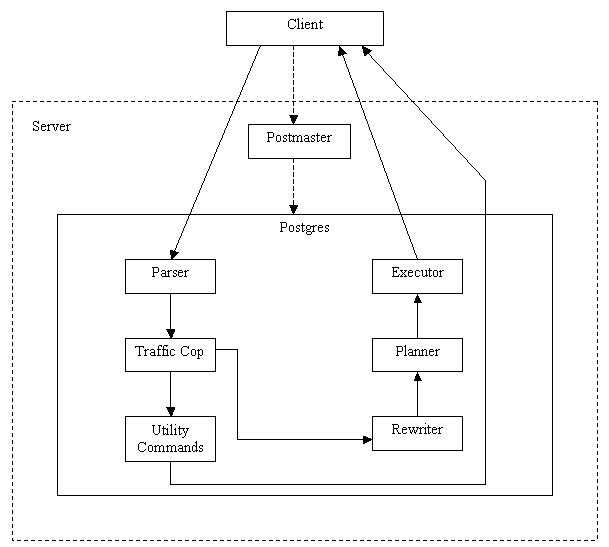
\includegraphics[width=0.6\textwidth]{./img/implementace/postgremodel1.jpg}
    \caption[Dotaz PostgreSQL]{\centering  Zpracování dotazu \footnotemark}
 \end{figure} 
   \label{tab:dotaz}
\footnotetext{\url{http://reshmaparveen.blogspot.cz/2009/12/normal-0-false-false-false.html}}
 %%% MK: comment end
\end{comment}

\subsubsection{Vlastnosti}
PostgreSQL je systém relační databáze doplněný o objektově orientovaný
model. Ten je specifikován v rozšíření standardu SQL3 z roku
1999\cite{sql1999}. Objektový model podporuje objekty, třídy a
dědičnost v databázových schématech. Objektově-relační systém pro
správu databáze poskytuje střední cestu mezi relační a plně objektově
orientovanou databází. To umožňuje vytváření vlastních
datových typů a metod, které umožňují vyšší míru abstrakce. Nechybí
podpora implementace vlastních procedur buď s využitím 
jazyka PL/pgSQL nebo externí podpory C/C$++$ (knihovny libpq a
libpq$++$), Python (PyGreSQL) či Perl (pgsql\_perl5).


\paragraph{Objekty} umožňují vytváření nových datových typů, konverzí,
přetypování, indexů, funkcí, agregačních funkci, operátorů a dalších.

\paragraph*{Funkce} umožňují spouštění bloků kódu, které mohou být jak
v nativním jazyce PL/pgSQL, tak i v ostatních výše zmíněných
podporách. Funkce po spuštění vracejí výsledek v řádcích, tedy
tabulkou, kterou je možné využít k dalším příkazům. Podporuje
vytvoření vlastních funkcí či využití funkcí  standardní knihovny
PostgreSQL.

\paragraph*{Indexy} je možné vytvářet pomocí algoritmů
\textit{B-tree}, \textit{hash}, \textit{GiSTm} a \textit{GIN}
\footnote{\url{http://www.postgresql.org/docs/9.1/static/sql-createindex.html}},
nebo lze vytvářet i vlastní. Princip indexu spočívá ve vytvoření
specifického sloupce v~tabulce, jehož jediný úkol je optimalizovat
prohledávání daného sloupce.

\paragraph*{Pravidla} umožňují přepisování zpracovaného dotazu. 
Jedno z běžných použití je implementace pohledů, které logicky odkazují na vybrané sloupce v
jiných tabul\-kách. V \textit{PostgreSQL 9.3 } jsou nově implementované
materializované pohledy (\texttt{MATERIALIZED VIEW}), které
představují jak charakteristiky tabulky tak i pohledu. Data
materializovaných pohledů jsou fyzicky uloženy na disku. Jejich hlavní
výhodou je možnost  obnovení (\texttt{REFRESH})  tabulky na základě logických vazeb z jejího vytvoření.

\paragraph*{Triggery} (spouštěče) mají funkcionalitu v podobě kontroly
událostí, na které reagují podle své definice. Například při vytvoření
nového záznamu provedou definovanou operaci v databázi.

\paragraph*{Datové typy} definují druh nebo význam hodnot.
PostgreSQL disponuje značným rozsahem datových formátů. Specifickými pro tuto
práci jsou: numerické, časové, logické, řadící (enumerate) a
geometrické typy.

\subsection{Extenze PostGIS}
\label{subsec:postgis}
PostGIS\footnote{\url{http://postgis.net/}} je open-source rozšířením
(\texttt{EXTENSION}) databáze PostgreSQL o podporu geografických
objektů. Jde tedy o velice vhodný nástroj pro využití v GIS. PostGIS
implementuje specifikaci \textit{Simple Features for
  SQL}\footnote{\url{http://www.opengeospatial.org/standards/sfs} }
konsorcia \acs{OGC}, která v současné době plní funkci standardizační
organizace pro geoprostorová data. PostGIS je 2D/3D vektorovou
databázovou nadstavbou, vedle které existuje i extenze PostGIS Raster pro data rastrová.

  
\begin{figure}[h!]
    \centering
    
\includegraphics[width=0.2\textwidth]{./img/implementace/postgis.png}
    \caption[Logo PostGIS]{\centering  Logo PostGIS \footnotemark}
 \end{figure}   
\footnotetext{\url{http://postgis.net/docs/manual-2.1/}}

\paragraph*{Prostorový model} 
je založen na specifikaci    \acs{OGC} \textit{Simple Feature}, z toho
plyne že model nepodporuje geometrickou topologii. OGC definuje
jednotlivé operace mezi standardem SQL a prostorovými daty. Souřadnice
jednotlivých objektů jsou ukládány v tabulkách, kde každá tabulka je
specifická jedním typem geometrie (bod, linie, polygon atd.) a
referenčním prostorovým systémem \cite{postgis}. 
%%% ML: WKT rozhodne, tu vetu bych klidne vynechal
%Souřadnice jsou ukládány ve standardu    \acs{WKT}.
%%% ML: tahle veta je zmatecna, prozatim zakomentovano
% Společně s metadaty  geometrického prvku jsou
% ukládány ve sloupci \texttt{geometry}, který má informaci o
% geometrickém typu o referenčním systému.
%%% MK: textu je dost, vynechame
%%% ML: OK

\paragraph*{Souřadnicový systém} je v PostGIS definován v tabulce
\texttt{SPATIAL\_REF\_SYS}. Obecně známé referenční souřadnicové systémy jsou již
předdefinované, ostatní se dají dodatečně definovat a upravovat.

\newpage %%% ML: fix poznamka pod carou

\begin{figure}[h!]
    \centering
    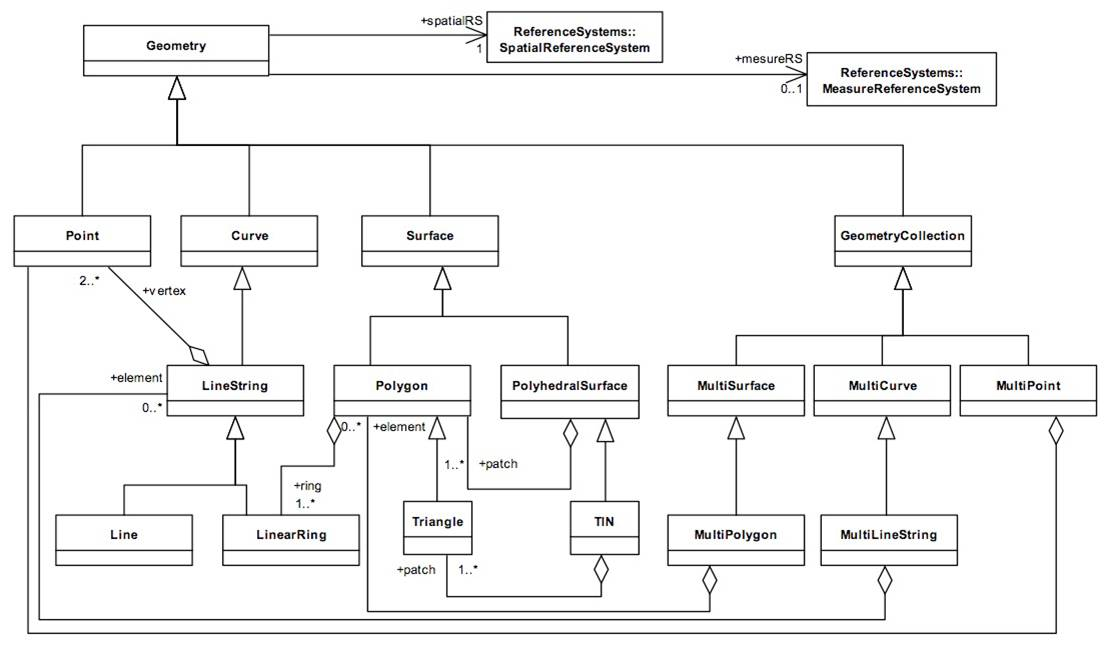
\includegraphics[width=1\textwidth]{./img/implementace/ogc1.jpg}
    \caption[Model PostGIS]{\centering Jednotlivé základní geometrické objekty 
    jsou agregovány do složitějších tzv.~multi objektů.     \footnotemark}
 \end{figure}   
%%% ML: odkaz pod carou je potom duplictni, poznamky pod carou se daji sdilet
%%% MK: tomuhle moc nerozumim. Jak to myslis?
%%% ML: je tam dvakrat poznamka pod carou se stejnym textem - http://www.opengeospatial.org/standards/sfs, kvuli preteceni obrazku na dalsi stranku, prohodil jsem odstavce
\footnotetext{\url{http://www.opengeospatial.org/standards/sfs}}

%%% ML: tohle bych uplne vynechal...
%%% MK: ok
% \begin{verbatim}
% CREATE TABLE spatial_ref_sys (
%   srid       INTEGER NOT NULL PRIMARY KEY,
%   auth_name  VARCHAR(256),
%   auth_srid  INTEGER,
%   srtext     VARCHAR(2048),
%   proj4text  VARCHAR(2048)
% )
% \end{verbatim}

Souřadnicové systémy jsou charakterizovány unikátním kódem
\texttt{\acs{SRID}}, který je všeobecně zažitým formátem v aplikacích GIS.
%%% ML: standardem?
%%% MK: muze to byt takhle?... který je všeobecně zažitým formátem v aplikacích GIS.
%%% ML: zacitym je spis EPSG (kteremu SRID v PostGISu i vetsinou odpovida...)
Pro konverze mezi jednotlivými systémy slouží funkce
\texttt{ST\_Transform}.
%%% ML: zbytecne
% \footnote{\url{http://postgis.org/docs/ST_Transform.html}}.
%%% MK: ok

\paragraph*{Geometrie} je datovým typem (\texttt{geometry}), který
představuje geometrickou složku popisu geoprvků.  Charakteristika tohoto
datového typu je dána standardem OGC \textit{Simple Features}.
%%% ML: data jsou ukladana v binarni forme (WKB ci odvozene) nikoliv ve WKT
%%% rovněž ve formátu \acs{WKT}.
%%% MK: no jasne. Chyba
Sloupec s geometrií je definován pomocí parametrů, které
nastavují obecná a geometrická specifika: název, typ, souřadnicový
systém apod.

Pro definování typu geoprvku jsou k vytvořeny funkce
\texttt{ST\_Make*}, kde \texttt{*} jsou níže uvedené typy standardu
%%% ML: todo - vysvetlit zkratku WKT
%%% MK: radek 841 je wkt poprve, dal jsem poznamku pod caru. Muze to tak byt? Nebo spis do textu?: "WKT je značkovací jazyk pro reprezentaci vektorových objektů na digitálních mapách."
%%% ML: OK
OGC \textit{Simple Features} (příklad v textové reprezentaci~\acs{WKT}):


\begin{verbatim}
POINT(0 0)                                               
LINESTRING(0 0,1 1,1 2)                                       
POLYGON((0 0,4 0,4 4,0 4,0 0),(1 1, 2 1, 2 2, 1 2,1 1))          
MULTIPOINT(0 0,1 2)                                              
MULTILINESTRING((0 0,1 1,1 2),(2 3,3 2,5 4))                       
MULTIPOLYGON(((0 0,4 0,4 4),(1 1,2 1,2 2)), ((-1 -1,-1 -2,-2 -2,))) 
GEOMETRYCOLLECTIONM(POINTM(2 3),LINESTRINGM(2 3,3 4))                
\end{verbatim}
\vskip-2ex
%%% ML: podobne jako PostgreSQL, kapitola mohla byt vyrazne KRATSI,
%%% ale nechme to tak jako je...
%%% MK: Tuto kapitolu bych nechal jak je, u kapitoly POSTGRESQL jsem pro neco SMAZAT.
%%% ML: nemam zasadnich namitek, i kdyz tu neni prima navaznost na text prace...
\paragraph*{Funkce} jsou v této nadstavbě zaměřeny na operace s
geometrií. Veškeré funkce mají prefix \texttt{ST\_} (\textit{spatial
  type}). Část z nich je funkčností analogicky odvozena z~nástrojů
GIS. Funkce jsou podle svého účelu roztříděny do kategorií. Níže jsou
demonstrovány jejich kategorie a nejzákladnější funkce.
\begin{description}
\item[Měřičské] funkce jsou typické pro prostorové výpočty: plocha
  \texttt{ST\_Area}, vzdálenost \texttt{ST\_distance}, vzdálenost na
  elipsoidu \texttt{ST\_length\_spheroid} a další.

\item[Geometrické konstruktory] slouží k vytváření geometrie podle
  \textit{Simple Features}, např: bodu \texttt{ST\_MakePoint},
  linie \texttt{ST\_MakeLine}, polygonu \texttt{ST\_MakePolygon} ad.

\item[Analytické] funkce jsou v PostGIS implementovány dle standardu
  ISO SQL-MM vyplý\-vající z ISO99, standard o multimédiích 
  \cite{sqlmm}. V této kategorii jsou funkce typické pro prostředí
  GIS. Mezi ně například patří: buffer \texttt{ST\_Buffer}, validita
  geometrie \texttt{ST\_IsValid} nebo sjednocení \texttt{ST\_Union}.

%%% ML: nejde o referencni (souradnicove) systemy ale formu zapisu geometrie
\item[Konverze] umožňují převod mezi různými formami zápisu geometrie (binárními a~textovými
  formáty). Například do rozšířeného formátu \acs{WKT}:

  %%% ML: tohle neni ciste WKT (tak jak se o nem mluvi ve OGC SF), ale
  %%% o rozsirenou formu PostGISu
  %%% MK: v PostGis manualu je psano WKT. Nevim jak to uchopit. Muze byt?: Například do rozšířeného formátu \acs{WKT}:
  %%% ML: OK
\begin{verbatim}
SELECT  ST_AsEWKT (geom) FROM link
.......
.......
"SRID=4326;LINESTRING(14.4533605575562 50.0689735412598,
                      14.4754581451416 50.0387687683105)"
\end{verbatim}
\vskip-2ex
\item[Agregační] funkce PostGIS jsou v principu stejné jako ve
  standardu SQL (průměr, max, min) s tím rozdílem, že jsou zaměřeny na
  prostorová data. Příkladem je funkce pro sjednocení
  \texttt{ST\_Union}.
\end{description}




\newpage
\setcounter{footnote}{1}
\section{Časoprostorové analýzy}

Hlavním účelem GIS je vytvoření informačního systému, který umožňuje
získá\-vání, ukládání, analýzu a vizualizaci dat vztažených k povrchu
Země.  Všeobecně je však hlavním cílem vytváření operačních modelů
reálného světa, přičemž je pro modelo\-vání některých reálných procesů
nedílnou součástí časová složka.  Z histo\-rického pohledu vývoje GIS
je zřejmá primární orientace na řešení problémů
prostorových dat bez časové  složky. V prvních fázích rozvoje GIS
nemohla ani být tato otázka z hlediska tehdejších omezení IT
technologií i~matematických formulací řešena
\cite{geospatialanal}. Systém GRASS v nové verzi \textit{GRASS
  GIS 7} obsahuje zcela nově navržený balíček modulů
%%% ML: tady bych vysvetlil zkratku TGRASS
%%% MK: muze byt formou zkratky?
%%% ML: OK
\acs{TGRASS} \footnote{\url{http://grass.osgeo.org/grass70/manuals/temporalintro.html}},
který integruje do původního GRASS systému časový rozměr.

Hlavním obsahem této kapitoly je představení časoprostorových
datových modelů s primárním zaměřením na model, který je implementován
v modulech TGRASS. V~praktické části budou představeny základní funkce
a analýzy TGRASS pro  srážky zrekonstruované pomocí vlastního modulu
\texttt{r.mwprecip}. K teoretické části byla jako primární zdroj
využita kniha \textit{Geographical information system vol.2} \cite{gistemporal}.


\subsection{Terminologie}
\label{subsec:terminologie}
Tento odstavec pojednává o základní terminologii časoprostorové
problematiky v GIS. Hlavním zdrojem  definic je publikace
\cite{pelekis}.
\begin{description}
\item[Reprezentace času] -- jednotlivé stavy geodat jsou odkazovány k
  časovým okam\-žikům dvěma způsoby - relativně (\textit{dny, roky,
    minuty}) či absolutně (\textit{1990-30-06 1:35:59}). Možností
  relativní reprezentace je vyjádření času v záporné notaci
  (\textit{-rok}). Další reprezentace je vyjádřena pomocí 
  dělení času (\textit {před -- minulý, teď -- současný, po -- budoucí}).

\item[Diskrétně časový model] je takový model, kde se proměnné, tedy
  geodata mění skokově. Geodata jednotlivých okamžiků na sebe navazují
  podle dostupného či zvoleného časového
  rozlišení (granularity). Názorným příkladem je sčítání lidu v daném časovém
  intervalu.

\item[Kontinuální/spojitý časový model] je charakteristický 
  jemným časovým rozli\-šením. Příkladem jsou data získaná ze
  seismografu či kontinuálního záznamu průtoku ve vodních tocích.

\item[Časová topologie] je termín, který je analogický k termínu
  prostorová topologie s~tím rozdílem, že kromě prostorového zobrazení zavádí i rozměr časový. Časová topologie geodat definuje vztahy
  mezi jednotlivými stavy daných objektů v datasetu.

\item[Granularita] je ve spojení s časoprostorovými daty definována
  jako velikost zákla\-dního časového intervalu na časové
  ose. 
\end{description}

\subsection{Časoprostorové modely}

Časoprostorové modely se liší v jednotlivém pojetí vztahů, které
propojují časovou složku s prostorovými daty. Současný vývoj a
specifické nároky vědních oborů vytvořily poměrně značný počet
časoprostorových modelů \cite{pelekis}, které jsou často sjednoceny
základní myšlenkou a liší se pouze v detailu. Níže jsou přiblíženy
principy základních modelů se zaměřením na \textit{Snapshot model},
který je použit jako časoprostorový model v TGRASS.

\subsubsection*{Snapshot model}
Jedná se o jeden z  nejednodušších a nejvyužívanějších časoprostorových
modelů. U tohoto modelu je začlenění časových složek aplikováno pomocí
relačního modelu, který je charakteristický relačními tabulkami, tedy
členěním daných vektorových či rastrových rámců do jednotlivých
časových vrstev/tabulek.

\begin{figure}[h!]
    \centering
    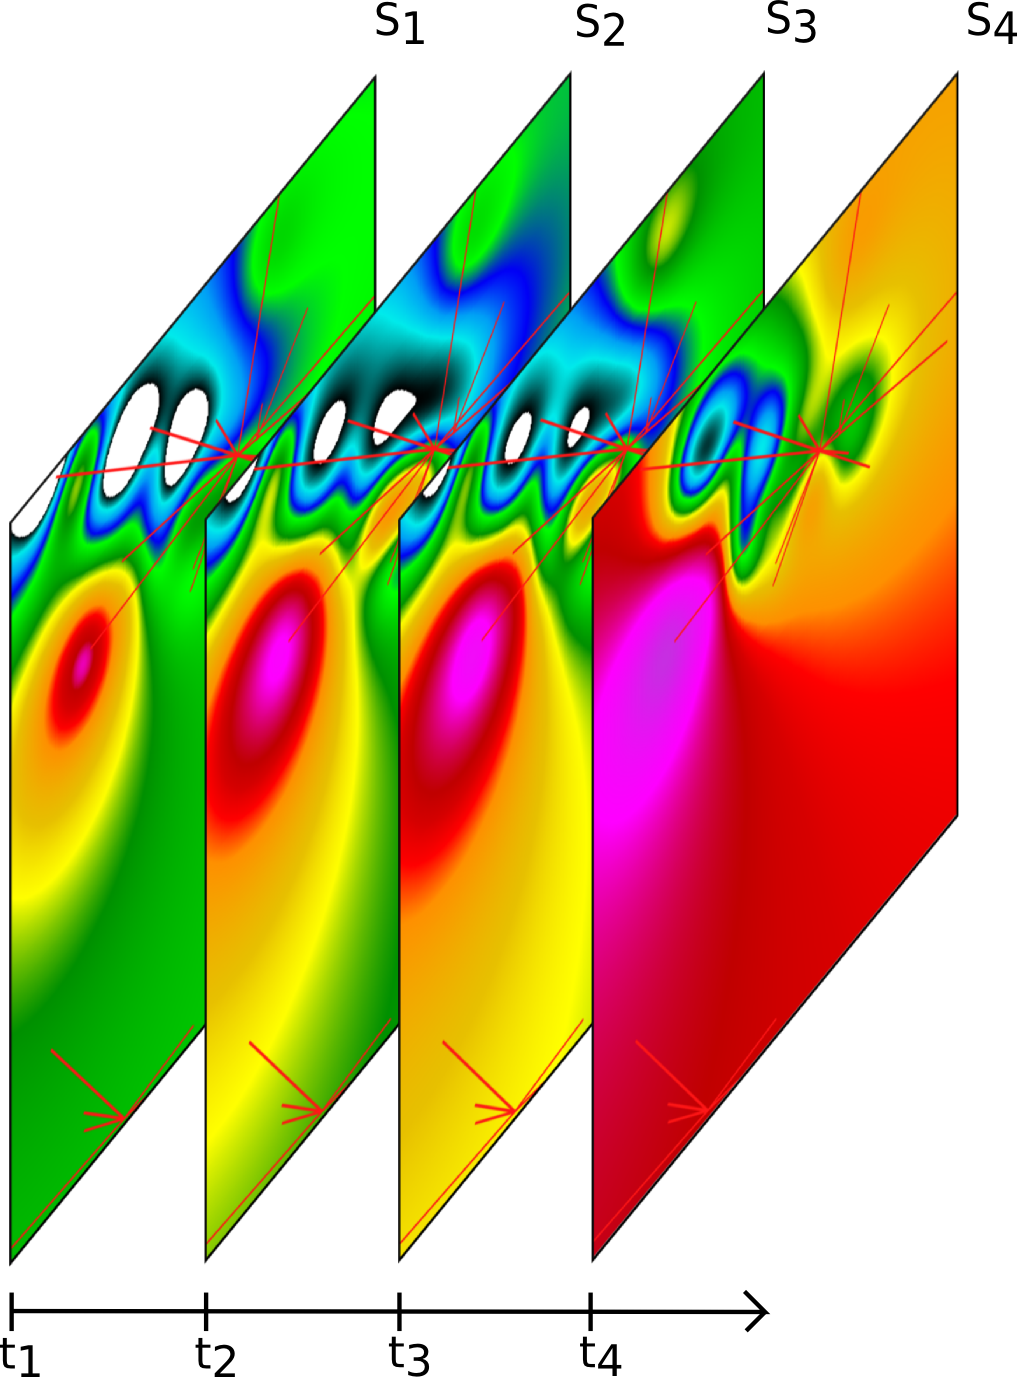
\includegraphics[width=0.3\textwidth]{./img/temporal/snapshot.png}
    \caption[Snapshot model]{Jednotlivé snímky \emph{S} reprezentují  geodata v čase \emph{t}. Obrázek schématicky znázorňuje vývoj dešťových srážek  \centering \footnotemark. }
        \label{fig:snapshot}
 \end{figure}   
\footnotetext{Podkladem pro obrázek byly využity výstupy z modulu {\tt r.mwprecip} (viz praktická část práce).}

Výhodou \textit{snapshot} modelu je jeho jednoduchost a především
vhodná struktura pro implementaci do GIS. Jak již bylo zmíněno, model
uchovává jednotlivé vrstvy pro dané časové okamžiky odděleně.
Jednotlivé tématické informace o zájmových oblastech jsou ukládány do
separovaných datových vrstev \ref{fig:snapshot}.  Model
charakte\-ristikou svého návrhu odpovídá diskrétním
systémům. Jednotlivé proměnné - geodata se skokově mění v průběhu
času. Z toho mimo jiné pro uplatnění v GIS plyne, že jednotlivé snímky
nemají informace o stavech předchozího či následujícího časového
okamžiku.  Nevýhodou tohoto modelu je proto datová redundance, která
je způsobena ukládáním informací pro daný okamžik vždy v plném
rozsahu.  Jednotlivá geodata jsou uchovávána pro časové okamžiky
nenávazně na předchozích. Uvážíme-li pro názornost extrémní případ,
kdy časový dataset obsahuje vrstvy znázorňující jev, který byl v
průběhu času neměnný, tento model do úložiště počítače zapíše
několikanásobně stejné geoinformace. Tato skutečnost je pro práci v
GIS poměrně nevýhodná, především v případech kdy změny sledovaných
veličin časoprostorových dat mezi jednotlivými okamžiky měření jsou
malé. Obecně se v oblasti numeri\-ckého modelování hydrologických i
meteorologických jevů jedná o častý tzv. {\em scaling} problém,
spočívající v potřebě interpretovat průběh různých stavových veličin
modelu (v tomto případě např. srážek) značně rozdílného časového
vývoje. Mezi nevýhody diskrétního modelování patří skoková
interpretace zobrazování procesů svou fyzikální podstatou původně
spojitých. V časoprostorovém kontextu při využití GIS modelů tohoto
typu to může vyvolat výpočetní stav, při němž dojde k igno\-rování
zásadní změny hodnoty sledované veličiny (např. srážky) v okamžiku
nepostihnutelném při zvoleném časovém intervalu měření.  Změna ovšem
nebude zaznamenána a model založený na těchto předpokladech bude v
praxi nepoužitelný. S~ohledem na potřebu porovnávání změn
jednotlivých prostorových rámců v čase je díky architektuře modelu
nutnost procházení a porovnávání buňky po buňce. To ovšem vede k
vysoké výpočetní náročnosti.

\paragraph*{Time Composit}
\textit{\ac{STC}} byl vyvinut v~roce
1988, Lagran \cite{lagran}. Model \acs{STC} pracuje s vektorovou interpretací
 prostorových dat. Jeho princip  spočívá v zobrazení linií do roviny, čímž se v~průběhu času jednotlivé prostory v projekční rovině sjednotí a tím z
nich vznikají polygony -- síť. V databázi jsou pak pro jednotlivé
polygony uchovávány atributy, které odpovídají jejich historii. Tento model
patří mezi diskrétní systémy, kde jednotlivé časové skoky
jsou relativní.

\paragraph*{Time-stamping model} 
Princip modelu je založen na dvojici časových razítek, které
určují čas vzniku a zániku či současného stavu
objektu. Časové razítko zániku objektu je definováno třemi stavy
\texttt{now}, \texttt{currnetm} a \texttt{null}.  Síla tohoto modelu
je při aplikacích, kde se jednotlivé objekty v průběhu dlouhé doby
mění sporadicky. Model byl navržen a otestován na katastru
nemovitostí, kde požadavky přesně odpovídají funkcím tohoto
modelu \cite{hunter}.

\paragraph*{Event model}
\textit{Event-Oriented Model} je svým principem podobný modelu Time-stamping. Model \textit{Time-stamping }nedokáže identifikovat jednotlivé změny v
rámci datasetu. Oproti tomu je  rozšířený o logovací
soubor, do kterého jsou zaznamenávány jednotlivé časové instance
objektů. Tento soubor představuje časovou topologii, která
reprezentuje celou historii změn objektů.
% a ten je možné procházet či
%analyzovat.

\paragraph*{Object-Relationship}
jako jediný z výše zmíněných datových modelů se zaměřuje na vztahy a popis
jednotlivých změn stavu sledované veličiny. Object-Relationship model je   specifický dle zaměření
dané problematiky. Jeho specifikem  je  náročnost v~definování
jednotlivých vztahů mezi objekty.

\paragraph*{Objektově orientovaný model}
\textit{Object-Oriented model}  lze svou filosofií přirovnat k objektově 
orientovaným programovacím jazykům. Umožňuje vytvářet
objekty, třídy, metody, instance, dědičnost, operátory a dynamické
vazby, tedy vše podstatné pro objektově orientovaný návrh. Díky tomu model umožňuje  uceleně simulovat reálné vztahy.  Jednotlivé objekty
v průběhu času ukládají své entity, které tak tvoří historii
instancí. Výhodou objektově orientovaného modelu je možnost jednoduchého a
intuitivního přístupu k jednotlivým informacím.


\subsection{Úvod do Temporal GRASS framework}
Temporal framework v systému GRASS (TGRASS) je součástí nové verze GRASS GIS 7. Je
implementován v jazyku C a Python. Data, která spravuje, jsou ukládána buď
v databázi SQLite nebo PostgreSQL. Nejčastěji je však
využívána výchozí databáze SQLite.

TGRASS je založen na tzv. {\em snapshot modelu} a dělí se na dvě úrovně:
časovou a~prostorovou složku. Prostorová složka je převzata ze systému GRASS a je
charakterizována 2D/3D vektorovými a rastrovými mapami. Jednotlivé
geoprvky s časovou charakteristikou jsou pak ukládány do časoprostorových
datasetů, které jsou specifické přiřazením časové známky či časových
intervalů.

\subsubsection{Koncept} 
Koncept vychází z části již představené terminologie časoprostorových
modelů. Je důležité pochopit základní charakteristiky časových závislostí,
granularity a časové topologie.

\paragraph*{Okamžik a interval} charakterizují dva přístupy k časovému
modelu.  Časový okamžik charakterizuje jeden moment v čase, oproti
tomu interval je definován počátečním  a koncovým okamžikem nebo pouze
počátečním časovým bodem a délkou intervalu.

\paragraph*{Absolutní a relativní} jsou definovány v TGRASS obdobně
jako kap. \ref{subsec:terminologie}.

\paragraph*{Granularita} tj. podrobnost časového rozlišení je v TGRASS
přepočítána po každém zásahu do datasetu. Mezi vlastnosti granularity
patří i vlastnost, kdy jednotlivé datasety obsahují mezery v čase
(gaps), ve kterých nejsou dostupná data.


\paragraph*{Časová topologie} v problematice časové proměnné
závislosti vychází obecně z~principu obecné topologie. Časová
topologie popisuje vztahy mezi jednotlivými časovými známkami jak pro
časový interval\ref{fig:topology} tak pro časový okamžik. Jednotlivé charakteristiky
byly odvozeny z booleovské algebry a aplikovány na časové známky.
\begin{figure}[h!]
    \centering
    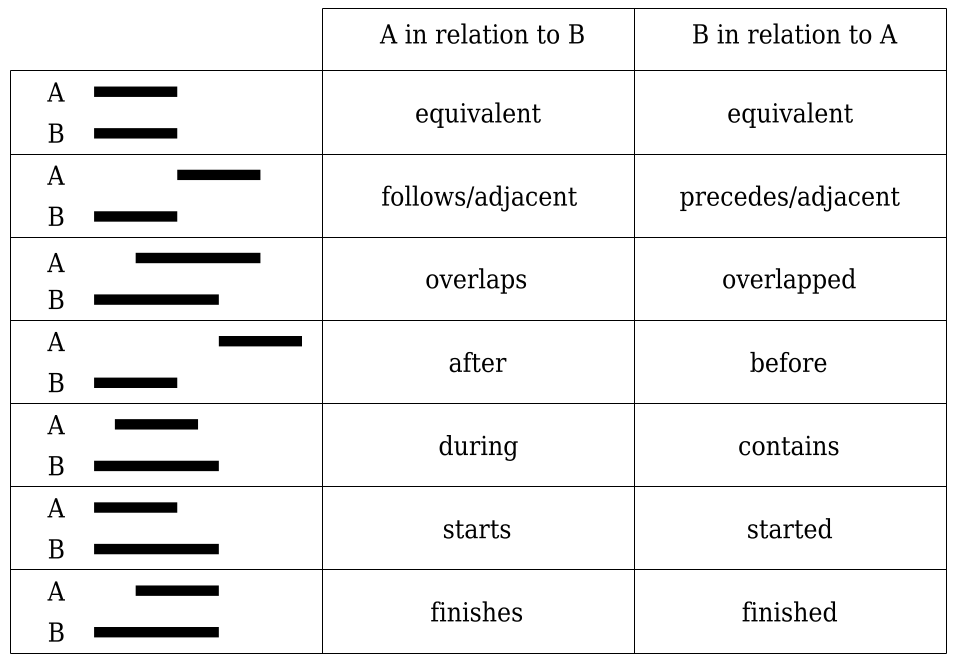
\includegraphics[width=0.7\textwidth]{./img/temporal/topology.png}
    \caption[Temporal sampling]{ Vztahy mezi časovými intervaly podle Allen, 1983. Zdroj obrázku: \cite{soren}. \centering  }
        \label{fig:topology}
 \end{figure}   

\paragraph*{Temporal sampling} vychází z časové topologie a určuje
jednotlivé vztahy mezi časovými datasety\ref{fig:sampling}. Pro představu jsou uvedeny
některé vztahy pro časové datasety např. h a B následující: start
(A, B mají stejný začátek), during (A během B), overlap (A, B se v
čase překrývají ), contain (A obsahuje B), equal (A a B jsou stejné),
follows (A je za B).



%%% ML: tady by se hodil obrazek prostorovych vztahu ze Soerenovych
%%% materialu (s prislusnou citaci...)
%%% MK:
%%% ML: OK
\begin{figure}[h!]
    \centering
    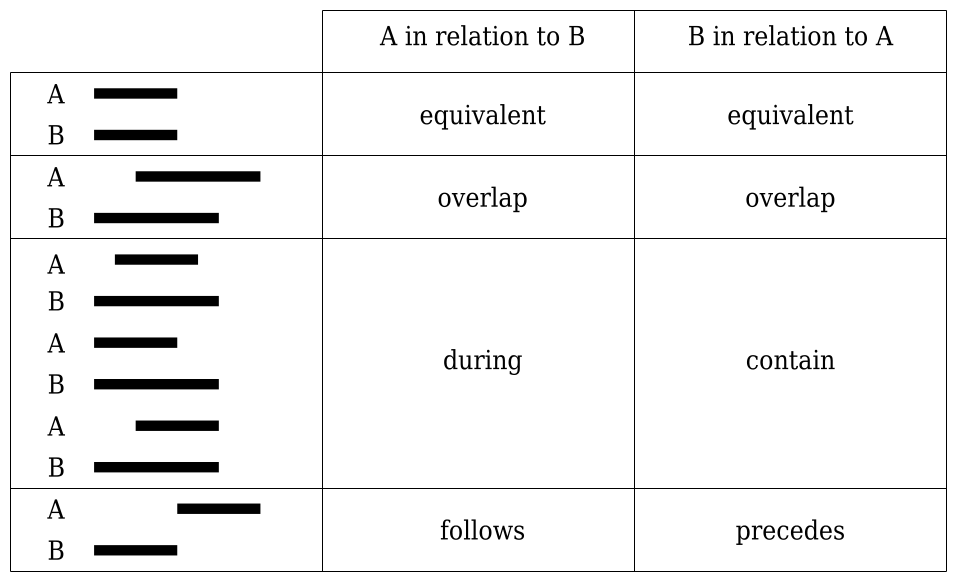
\includegraphics[width=0.7\textwidth]{./img/temporal/sampling.png}
    \caption[Temporal sampling]{Schema vztahů pro temporal sampling \cite{soren}.   \centering  }
        \label{fig:sampling}
 \end{figure}   

Pomocí těchto výroků lze definovat výběr \uv{časových oken} z datasetu A
na základě datasetu B (např. průnik).













\newpage
\setcounter{footnote}{1}
\chapter*{Praktická část}\stepcounter{chapter}\addcontentsline{toc}{chapter}{Praktická část}
\setcounter{section}{3}

\noindent Hlavní směr praktické části je věnován vývoji vlastních GIS modulů, na něž jsou navázány další kroky této práce, které se zaměřují na charakterizaci aplikačního potenciálu.
Pro ucelený pohled na danou problematiku jsou v první kapitole \ref{sec:charakteristikadat} praktické části představeny charakteristiky vstupních dat.

Jednotlivé kapitoly praktické části  jsou seřazeny na základě chronologického postupu vývoje aplikací:
\begin{enumerate}
\item Charakteristika dat \ref{sec:charakteristikadat}  - analýza dostupných dat
\item Navržené nástroje do systému GRASS \ref{sec:grassgismodule} - návrh aplikace, implementace a ovládání
\item Výstupy modulů a jejich využití \ref{sec:vystupymoduluavyuziti} - testování aplikace 
\end{enumerate}



\setcounter{footnote}{1}
\section{Charakteristika dat}
Následující text popisuje obecné vlastnosti dat MV spojů s přímou návazností konkrétní analýzy 
dostupného vzorku dat pro tuto práci.

\label{sec:charakteristikadat}
V současné době je v rámci zadavatelského projektu  využíváno naměřených dat z
MV spojů od telekomunikačního operátora T-Mobile, která jsou ukládána
do databáze PostgreSQL.

\subsection*{Data}  
 
Od dubna 2013 jsou sbírána data z 14 MV spojů na pilotním povodí
projektu v~Praze Letňanech a 7 spojů na území Prahy Michle a
okolí. Zároveň jsou k dispozici 3 referenční srážkoměry v okolí MV
spojů v Letňanech.  V současné době se pracuje na dohodě o poskytování
dat většího pokrytí území hl.m. Prahy.

Data jsou v současné době\footnote{situace v květnu 2014} sbírána ze sítě která se skládá ze dvou uzlů a jejich příslušných spojů.

\begin{figure}[h!]
    \centering
    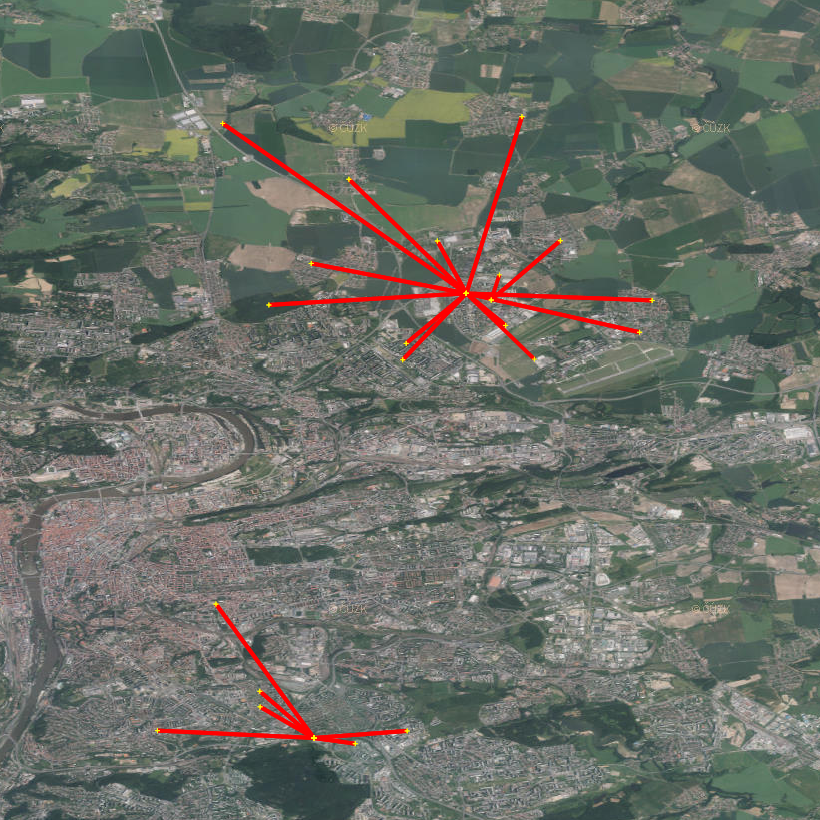
\includegraphics[width=0.5\textwidth]{./img/letnany.png}
    \caption[Snapshot model]{Současný stav MV spojů dostupných v rámci projektu v lokalitě Praha  \centering  }
        \label{fig:snapshot}
 \end{figure} 

Časový krok je determinován odezvou jednotlivých 
zařízení, která jsou dotazována sériově. Pro sbírané množství je tak 
dosaženo časového kroku cca~12-15~s.

\subsection*{Databáze}  
Pro záznam měřených hodnot je využívána databáze
PostgreSQL, která běží na PC na ústředí T-Mobile připojenému na 
dohledovou síť operátora. 
 Záznam dat pro zmíněné lokality probíhá nepřetržitě od
dubna 2013. Dostupná data jsou ve formě zálohy databáze
(\textit{database dump}) časového rozsahu jednoho týdne
sběru. Databáze obsahuje tabulky \texttt{link}, \texttt{node} a
\texttt{record}.
 
 
\begin{comment}

\begin{table}[h!]
\centering
\begin{tabular}{|lll|}
\hline
\multicolumn{1}{|c}{tabulka} & \multicolumn{1}{c}{atributy}                                                    & \multicolumn{1}{c|}{popis} \\ \hline\hline
link   & \begin{tabular}[c]{@{}l@{}}linkid, rxoid, txoid\\ fromnode, tonode\end{tabular}    & definice spojů z vysílačů \\\hline
node   & \begin{tabular}[c]{@{}l@{}}ipaddres, lat, long \\ name, nodeid\end{tabular}        & geometrie vysílačů       \\\hline
record & \begin{tabular}[c]{@{}l@{}}linkid, time, frequency\\ rxpower, txpower\end{tabular} & naměřené hodnoty          \\ \hline
\end{tabular}
\caption{Přehled tabulek z databáze}
\label{tab:database}
\end{table}

\end{comment}


\paragraph*{Tabulka link} obsahuje informace, ze kterých vysílačů
(\texttt{fromnodeid, tonodeid}) jsou jednotlivé spoje
(\texttt{linkid}) definovány. Ostatní atributy nebyly využity.

\begin{figure}[h!]
\centering
\footnotesize
\begin{BVerbatim}
 linkid |  ifname  |   rxoid    |   txoid    | fromnodeid | tonodeid 
--------+----------+------------+------------+------------+----------
     43 | 1/2.1/1  | 2129920257 | 2146697473 |         23 |       29
     44 | 1/16.1/1 | 2129922049 | 2146699265 |         29 |       23
     45 | 1/2.1/1  | 2129920257 | 2146697473 |         24 |       29
     46 | 1/6.1/1  | 2129920769 | 2146697985 |         29 |       24
\end{BVerbatim}
\caption{ Výpis dat z tabulky  \texttt{link} (limit 4) }
\end{figure}


\paragraph*{Tabulka node} obsahuje klíčové informace o poloze vysílačů
v souřadnicovém systému WGS-84 (\texttt{lat, long}) -- EPSG 4326.

\begin{figure}[h!]
\centering
\footnotesize
\begin{BVerbatim}
   ipaddress   |   lat   |  long   |  name  | nodeid 
---------------+---------+---------+--------+--------
 10.230.79.65  |  50.069 | 14.4534 | 10283A |     23
 10.230.79.93  | 50.0375 | 14.4848 | 10333A |     24
 10.230.80.245 | 50.0404 | 14.4965 | 12209A |     25
 10.230.79.69  | 50.0458 | 14.4633 | 12276A |     26
\end{BVerbatim}
\caption{Výpis dat z tabulky  \texttt{node} (limit 4)}
\end{figure}

\paragraph*{Tabulka record} má atributy \texttt{time} datového typu
\texttt{timestamp}; \texttt{rxpower} a \texttt{txpower}  v nichž jsou údaje o
odeslané a přijaté intenzitě signálu.

\begin{figure}[h!]
\centering
\footnotesize
\begin{BVerbatim}
 linkid |          time           | rxpower | txpower 
--------+-------------------------+---------+---------
     43 | 2013-09-08 23:59:14.913 |   -48.5 |      -3
     45 | 2013-09-08 23:59:15.334 |   -48.5 |      -4
     47 | 2013-09-08 23:59:15.755 |   -48.9 |       2
     49 | 2013-09-08 23:59:16.161 |   -48.9 |      -7
\end{BVerbatim}
\caption{Výpis dat z tabulky \texttt{record} (limit 4) }
\end{figure}




V současné době není do databáze zahrnut atribut s hodnotami o vertikální či
horizontální pola\-rizaci signálu (\texttt{polarization}). 
Tyto hodnoty byly přidány do databáze z externího zdroje informací. 
%%% ML: tato cast vety mi nedava smysl, neco tam chybi...
%%% MK: opraveno
%%% ML: OK
V současné době probíhá jednání se správcem databáze
T-Mobile o přidání tohoto atributu.
 


\section{Navržené nástroje pro systém GRASS}
\label{sec:grassgismodule}
Jedním z hlavních výstupů této práce je návrh a implementace
modulu \textit{r.mwprecip} pro zpracování hrubých dat z MV spojů v
GIS. K tomuto účelu byl zvolen systém GRASS GIS s využitím rozhraní
\textit{GRASS Python Scripting Library}. V rámci vývoje byly vytvořeny
dva moduly:



\begin{itemize}
\item {\it r.mwprecip} je modul, který tvoří hlavní GIS nástroj pro
  zpracování dat MV spojů uložených v databázi.
  

\item {\it v.link.precip} je doplňkovým modulem k \textit{r.mwprecip},
  jehož funkčnost spočívá v nativním přístupu k výsledkům v GRASS
  GIS.
\end{itemize}

\begin{figure}[h!]
    \centering
    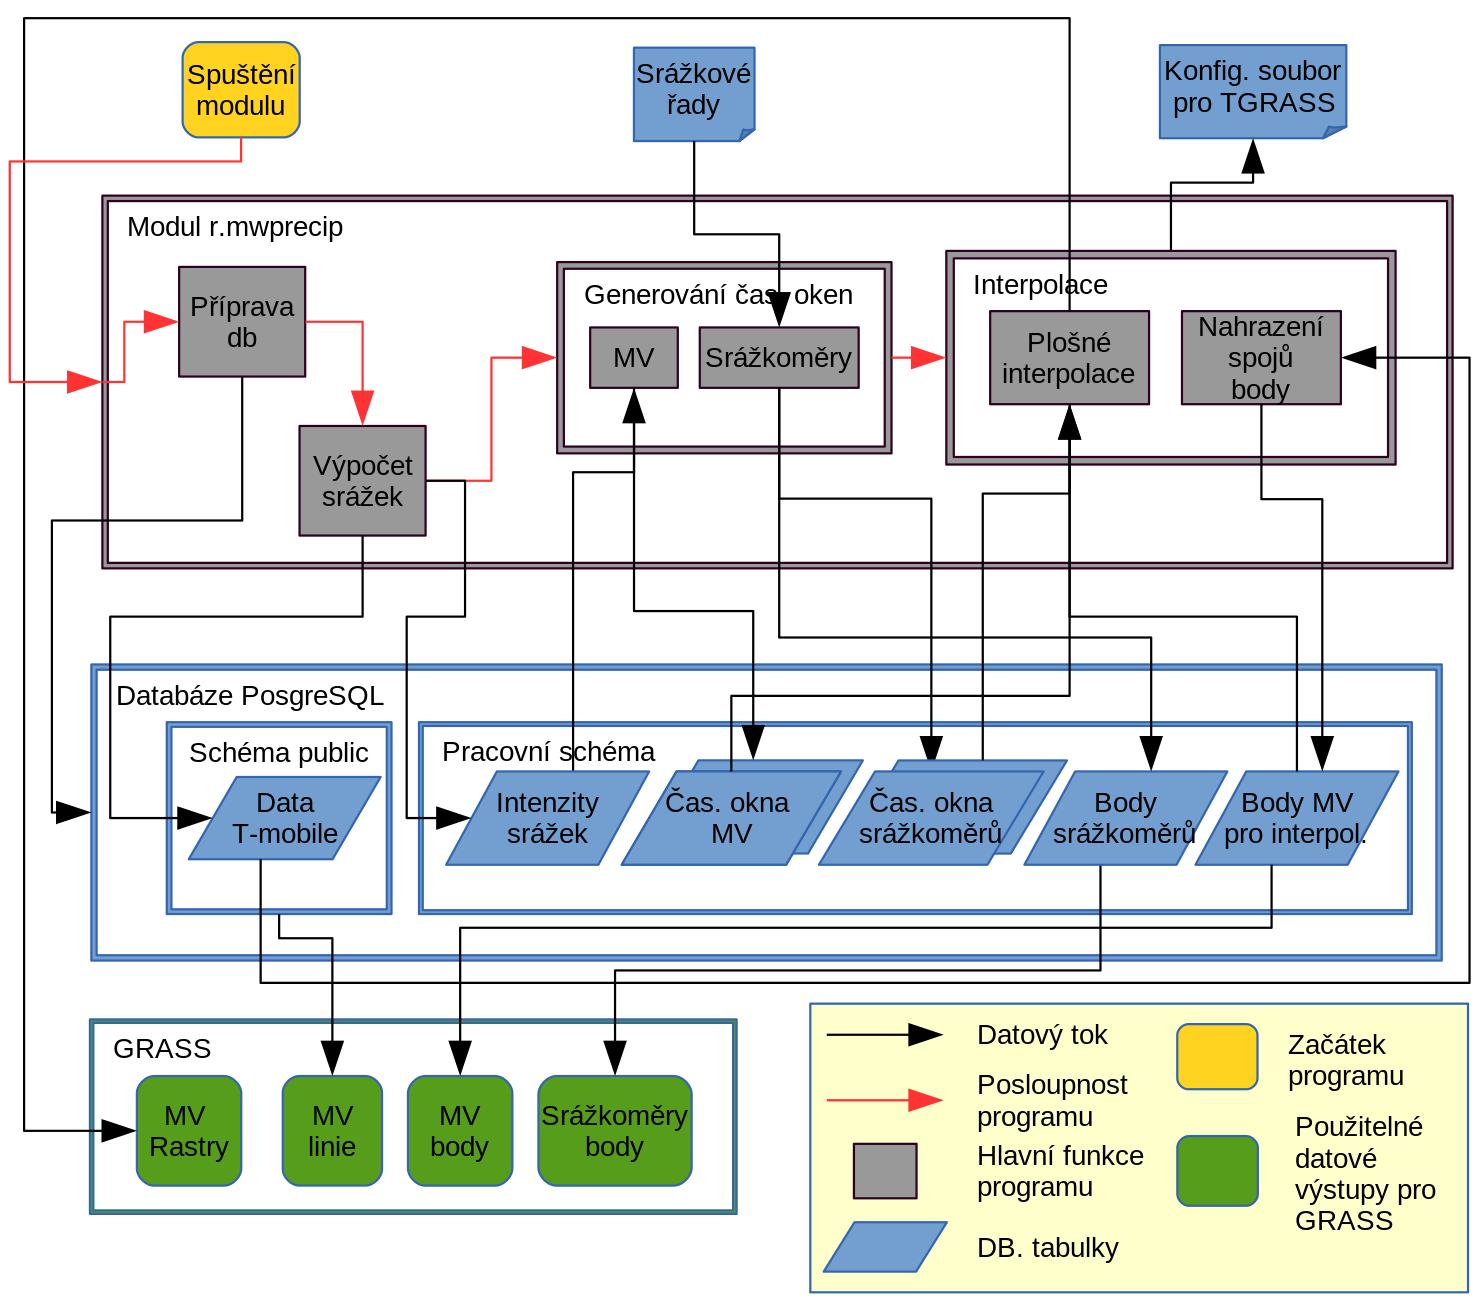
\includegraphics[width=1\textwidth]{./img/grass/diagram.png}
    \caption[GUI modul]{Schéma programu a jeho datových toků  \centering  }
        \label{fig:schema1}
\end{figure}



 
\begin{figure}[h!]
    \centering
    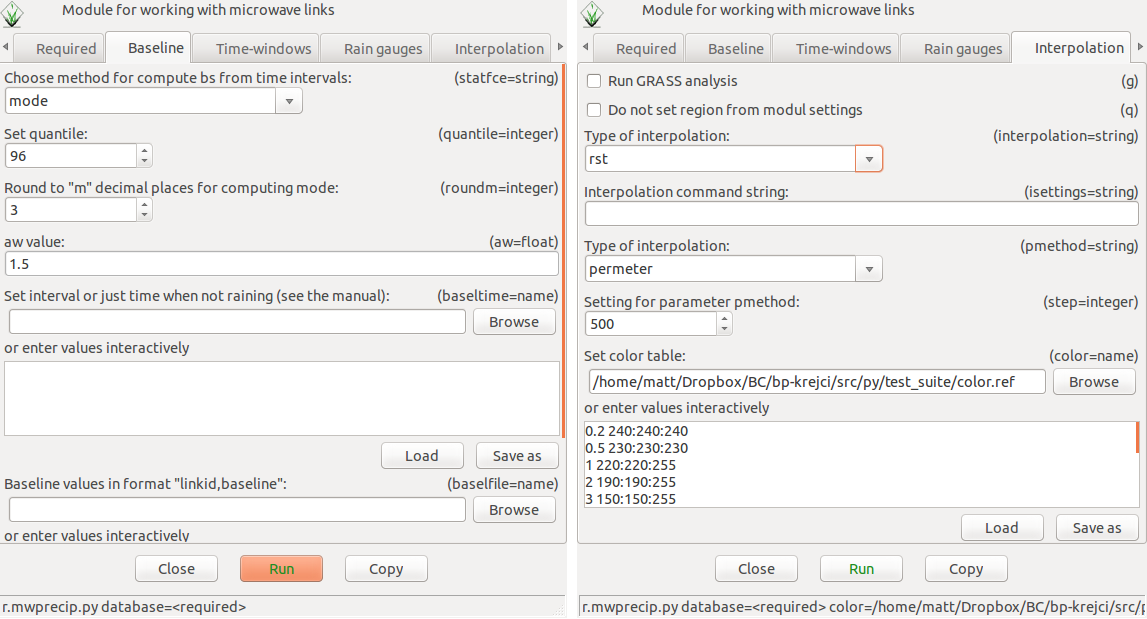
\includegraphics[width=0.9\textwidth]{./img/grass/gui.png}
    \caption[GUI modul]{Ukázka GUI r.mwprecip sekce Baseline a Interpolation  \centering  }
        \label{fig:baseline}
 \end{figure}

\paragraph*{Použité knihovny} Při psaní programu bylo využito jazyka Python, který je podporován
knihovnou \textit{GRASS Python Scripting Library} \cite{spygrass}. Ta
umožňuje volání GRASS modulů. Mimo to bylo využito dílčích funkcí standardní
knihovny \textit{The Python Standard
  Library}\footnote{\url{https://docs.python.org/3.4/library/}}.

Knihovna \textit{psycopg}\footnote{\url{http://initd.org/psycopg/docs/}}
umožňuje v jazyce Python přístup k databázi PostgreSQL. Této knihovny
bylo využito pro veškerý přístup do databáze s výjimkou přístupu z~GRASS
modulů volaných z \textit{GRASS Python Scripting Library}.

\paragraph*{Uživatelské rozhraní}
Uživatelské rozhraní navržených modulů je definováno sadou přepínačů
a~ para\-metrů, viz kap. \ref{subsubsec:grassterminologie}. Program se
ovládá (spouští) buď z příkazové řádky GRASS nebo ve wxGUI, kde se
vygeneruje dialogové okno s jednotlivými předem nakonfigu\-rovanými
sekcemi.




\subsection{Modul r.mwprecip}
Primární účel modulu \textit{r.mwprecip} je ve vytvoření rozhraní, 
pomocí kterého je možno zpracovat hrubá data MV
spojů do vhodných formátů pro analýzy v GRASS.


\paragraph{Funkce} modulu spočívají jak ve zpracování dat, tak ve
výstupu vhodném pro další GIS analýzy. Modul pro výstupní data podporuje dvě
základní reprezentace dat. Výstupem jsou interpolované
srážky v rastrové podobě a vektorová reprezentace pro jednotlivé MV
spoje.  K zpracování a analýzám dlouhých časových řad ve zvoleném intervalu je
výhodné využít balíčku časoprostorových modulů (TGRASS), které jsou nově v \textit{GRASS
  GIS 7} . Výstupní data z modulu \textit{r.mwprecip} jsou v kompatibilním formátu s TGRASS. 
  Součástí plné kompatibility jsou automaticky předpřipraveny nutné 
registrační soubory do uživatelské pracovní složky.  

Funkčnost modulu je možné rozdělit do hlavních čtyř skupin, 
které charakterizují vlastnosti modulu. 
Na obrázku \ref{fig:schema1} je znázorněn základní princip fungování modulu a 
jeho  datových toků mezi databází, modulem a rozhraním systému GRASS. 
 Zmíněné skupiny funkcí mají následující chronologický postup:
\begin{enumerate}
\item \textbf{data} - konfigurace a přístup
\item \textbf{výpočet srážek}	 - intenzity srážek z MV spojů
\item \textbf{generování časových oken}	 - vytvoření instancí MV spojů pro časové okamžiky
\item \textbf{interpolace} - vytvoření plošných interpolací z \uv{časových oken}
\end{enumerate}







V následujícím textu jsou obecně představeny  jednotlivé funkce modulu
\textit{r.mwprecip} a s tím spojená jejich možná konfigurace. Konkrétní ukázka nastavení modulu
 je v příloze \ref{appendix:ukazkakonf}.
Uživatelské rozhraní se primárně dělí na již zmíněné čtyři části a následující text  je podle tohoto dělení strukturován.

\subsubsection*{Data}
V následujícím textu je popsána příprava databáze a filozofie správy dat. 

\paragraph*{Příprava databáze}
 se provádí automaticky v prostředí navrženého GRASS mo\-dulu a 
 skládá se z jednotlivých dílčích úkonů, které jsou na obecné úrovni popsány v praktické části \ref{subsec:postgis} a \ref{subsec:postgresql}. Úpravy databáze jsou: 
\begin{itemize}
%%% ML: odkaz na kapitolu o PostGISu
%%% MK: opraveno
%%% MK: OK, jemne upraveno
\item \textbf{Geometrie} - využití extenze PostGIS (viz kap. \ref{subsec:postgis}) k vytvoření geometrických prvků pro MV spoje v databázi.

\item \textbf{Indexy} - vytvoření indexů pro optimalizaci vyhledávání dotazů v databázi. K vytvoření indexů bylo využito algoritmu.
\textit{B-tree}. \footnote{\url{http://www.postgresql.org/docs/9.2/static/indexes-types.html}}.

\item \textbf{Funkce} - přidání funkce v jazyku PL/pgSQL k agregaci hodnot daných sloupců a z nich výpočet statistické funkce modus. 

\item \textbf{Konfigurace} -  spočívá především v doplnění
atributů a vytvořením sekvencí v databázi.
\end{itemize}


%%% MK:start- zakomentovano na prani martina.
\begin{comment}
\paragraph*{Geometrie} Do databáze je přidána extenze PostGIS
(\texttt{CREATE EXTENSION post\-gis}), která umožňuje vytvořit
geometrický atribut (\texttt{geom}) u tabulky {\tt node} a
{\tt link}. 


\begin{footnotesize}
\begin{lstlisting}[style=mybash]
SELECT AddGeometryColumn ('public','node','geom',4326,'POINT',2)
\end{lstlisting}
\end{footnotesize}
\vskip-2ex
Vytvoření geometrického atributu ({\tt geom}) datového typu LINESTRING pro spoje. 

\begin{footnotesize}
\begin{lstlisting}[style=mybash]
SELECT AddGeometryColumn('public','link','geom',4326,'LINESTRING',2)
\end{lstlisting}
\end{footnotesize}
\vskip-2ex
Definování geometrie vysílače.

\begin{footnotesize}
\begin{lstlisting}[style=mybash]
UPDATE node SET geom = ST_SetSRID(ST_MakePoint(long, lat), 4326)
\end{lstlisting}
\end{footnotesize}
\vskip-2ex
Dále byla pomocí funkce \texttt{ST\_MakeLine} zrekonstruována geometrie
spojů (\texttt{link}) z vysí\-lačů (\texttt{node}). Z geometrie spojů
(\texttt{link}) byla vypočtena jejich délka funkcí
\texttt{ST\_Length}.

\paragraph*{Indexy} byly vytvořeny v tabulce \texttt{record} nad
atributy {\tt time} a {\tt recordid}, po optimalizaci dotazů nad tabulkou
{\tt record}. K vytvoření indexů bylo využito algoritmu
\textit{B-tree} \footnote{\url{http://www.postgresql.org/docs/9.2/static/indexes-types.html}}.

\begin{footnotesize}
\begin{lstlisting}[style=mybash]
--index b-tree pro atribut recordid
CREATE INDEX idindex ON record USING btree(recordid);		
\end{lstlisting}
\end{footnotesize}
\vskip-2ex
\paragraph*{Funkce} v nativním jazyku PL/pgSQL byla využita pro
agregaci hodnot pro daný sloupec ve zvolené tabulce k výpočtu
statistické funkce modus.

\paragraph*{Konfigurace tabulek} databáze spočívá především v doplnění
atributů vytvořením sekvencí a vymazáním záznamů $rxpower= -99.9$,
které charakterizují výpadek spoje.

\end{comment}
%%% MK: end-zakomentovano na prani martina.


Při každém uživatelském spuštění modulu \textit{r.mwprecip } proběhne
kontrola stavu databáze. Při zjištění prvního spuštění je databáze nakonfigurována.  Filosofie modulu je
založena na předpokladu, že bude sloužit k experimentálním pokusům
v~rozhraní GRASS GIS. Jednotlivé kroky výpočtů jsou od sebe odděleny
tak, aby se při změně parametrů části programu znovu nemusely provádět
veškeré výpočty. 

\paragraph*{Správa dat}
Modul pracuje v oddělených databázových schematech. Volbou pracovního
 schéma se vytvoří pracovní složka ve spouštěcím adresáři a databázové schéma v připojené databázi.
Vlastnosti správy dat se dají shrnout v následujících bodech:
\begin{description}
\item Z databázového schématu \texttt{public} načítá veškerá data z databáze a až na prvotní
jednorázovou přípravu databáze do něj nezapisuje. Výsledky modulu se zapisují odděleně do pracovního schématu, který si uživatel
pojmenuje pomocí parametru \texttt{schema}.

\item Volbou různých názvů
schémat je možné vytvářet jednotlivé pracovní instance daných konfigurací
výpočtů a zpětně se k nim vracet.

\item Modul zapisuje konfiguraci nastavených výpočtů do textových souborů,
které jsou uloženy ve složce s názvem zvoleným pro pracovní schéma
(parametr \texttt{schema}). Složka je umístěna ve spouštěcím adresáři
modulu. Při dalším spuštění modul porovnává nastavení s konfiguračními
soubory a na základě toho provede jen část výpočtu se změněnými
parametry.

\item  Smazání pracovního schématu lze docílit  v sekci \textit{Optional}  přepínačem \texttt{-r}, 
který smaže jak pracovní složku, tak schéma z databáze. Této funkce se může mimo jiné využít například
při nekorektním ukončení modulu či výpočtu. 
\end{description}
\begin{table}[h]
\centering
{\small
\begin{tabular}{|lll|}
\hline
\multicolumn{1}{|c}{sekce} & \multicolumn{1}{c}{parametry/ přepínače}                                                    & \multicolumn{1}{c|}{popis}    \\ \hline\hline
Required                   & {\tt database}                                                                                    & jméno databáze s daty         \\\hline
Baseline                   & \begin{tabular}[c]{@{}l@{}}{\tt statfce quantile roundm}\\{\tt aw baseltime baselfile}\end{tabular}    & nastavení výpočtu baseline   \\\hline
Time-windows               & \begin{tabular}[c]{@{}l@{}}{\tt interval fromtime}\\{\tt totime lignore}\end{tabular}                 & nastavení časových oken       \\\hline
Rain Gauges                & {\tt rgauges}                                                                                    & nastavení vstupu srážkoměrů   \\\hline
Interpolation              & \begin{tabular}[c]{@{}l@{}}{\tt -g -q interpolation}\\{\tt isettings pmetohod step color}\end{tabular} & nastavení interpolací a barev \\\hline
Database                   & {\tt user password}                                                                               & doplňkové nastavení db        \\\hline
Optional                   & {\tt -p -r schema}                                                                                & informace o db, smazání temp \\ \hline
\end{tabular}
}
\caption{Přehled parametrů v jednotlivých GUI sekcích}
\label{tab:rozhrani}
\end{table}


\subsubsection*{Výpočet srážek} 
Výpočet srážek a konfigurace se uživatelsky nastavuje 
v GUI sekci \textit{Baseline}. Zde jsou parametry pro konfiguraci výpočtu intenzit srážek,
kde se jedná především o parametry nastavující metody určení baseline \footnote{určení baseline: jde o určení hodnot útlumu MV signálu během suchého období, 
které je nutné znát pro výpočet intenzit srážek.}. Teoretickým východiskem pro 
určení baseline je kapitola, \ref{subsec:chyby} Mikrovlnné spoje. 

Baseline lze primárně určit dvěma způsoby. První metodou je přímé zadání známých hodnot ve formátu CSV. 
Druhý způsob  je umožněn pomocí volby suchého období a z něj spočtení hodnoty baseline na základě statistických funkcí. Schéma volby baseline je znázorněno na obrázku.  \ref{fig:schemabase}.

\begin{figure}[h!]
    \centering
    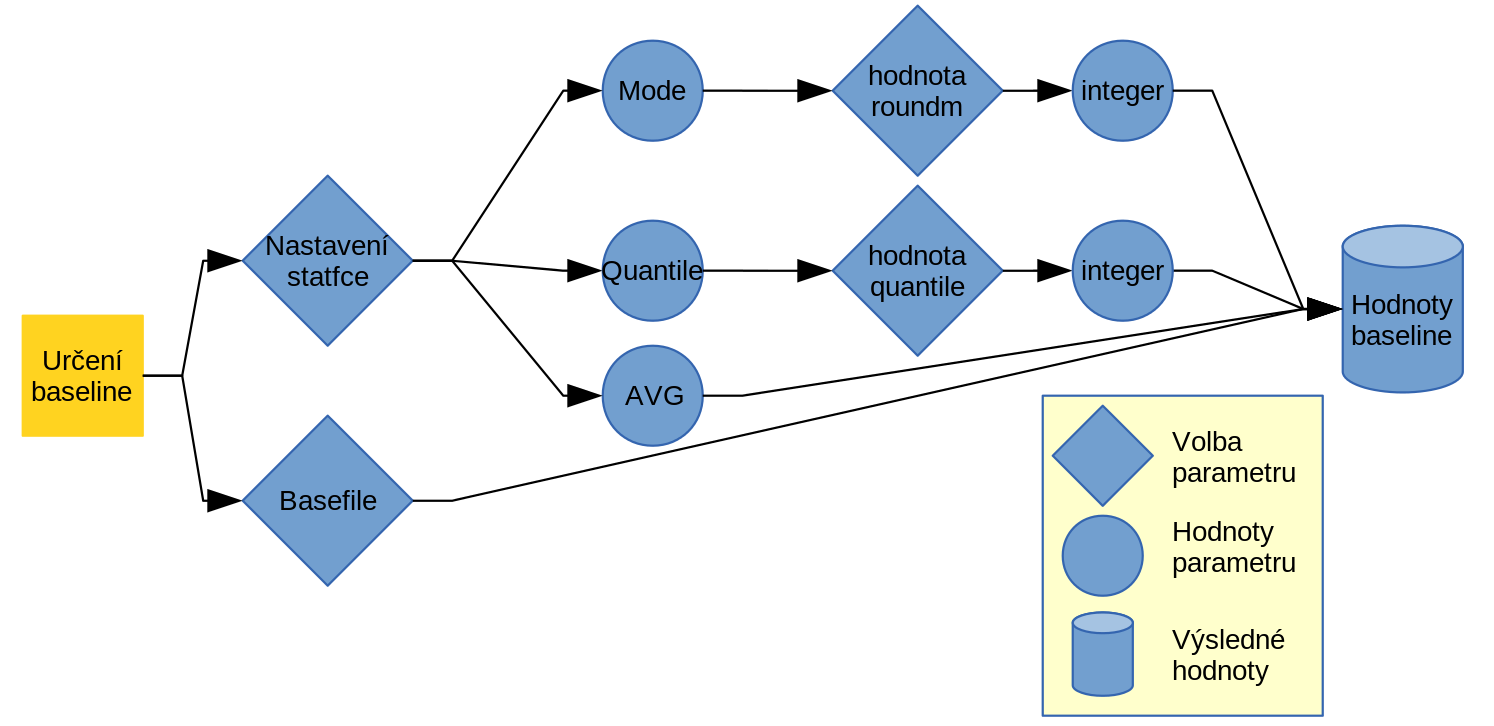
\includegraphics[width=1\textwidth]{./img/grass/baselinedia.png}
    \caption[GUI modul]{Schéma volby baseline  \centering  }
        \label{fig:schemabase}
\end{figure}



\paragraph*{Zadání známých hodnot} umožňuje \texttt{baselfile}, do kterého vstupuje textový soubor
s hodnotami identifikátorů spojů (\texttt{linkid}) a příslušnými
hodnotami baseline ve formátu \acs{CSV}.

\begin{table}[h!]
\centering
\begin{tabular}{|lll|}
\hline
\multicolumn{1}{|c}{parametr} & \multicolumn{1}{c}{typ} & \multicolumn{1}{c|}{explicitní hodnoty}                                \\ \hline\hline
{\tt statfce}                                & string                  & \begin{tabular}[c]{@{}c@{}}mode avg quantile\end{tabular}     \\
{\tt quantile}                               & integer                 & 1-100                                                         \\
{\tt roundm}                                 & integer                 & -                                                             \\
{\tt aw}                                     & float                   & -                                                             \\
{\tt baseltime}                              & soubor         		 & interaktivní zadání                                           \\
{\tt baselfile}                              & soubor         		 & interaktivní zadání                                           \\ \hline
\end{tabular}
\caption{Parametry v GUI sekci Baseline}
\label{my-label}
\end{table}

\paragraph*{Volbou suchých období}
je  možné definovat  časové intervaly nebo okamžiky, které slouží jako referenční hodnoty pro určení baseline. Z těch se následně zvolenými statistickými funkcemi vypočtou výsledné hodnoty.

Volba suchých období se definuje do textového souboru, který je vstupní hodnotou do parametru \texttt{baseltime}, např.: 

\begin{figure}[h!]
\begin{footnotesize}
\lstset{extendedchars=false,
escapeinside=''}
\begin{lstlisting}[style=mybash]
2013-09-09 07:00:00     -'č'asov'ý' okam'ž''i'k	
int                     -uvozen'í' intervalu
2013-09-10 04:00:00     -za'č''á'tek obdob'í'
2013-09-10 05:00:00     -konec obdob'í'
2013-09-13 04:55:00     -'č'asov'ý' okam'ž''i'k	
\end{lstlisting}
\end{footnotesize}
\end{figure}
\vskip-2ex
První řádek označuje časový okamžik suchého období, na
dalším řádku je časový interval uvozený řetězcem \texttt{int} a za ním
následují dva řádky definující interval. Další řádek reprezentuje
další zvolený časový okamžik.


Z vybraných suchých období se určují výsledné hodnoty \textit{baseline} pomocí základních statistických funkcí (parametr \texttt{statfce}):
\begin{itemize}
\item průměr - určení hodnot baseline prostým průměrováním hodnot pro jednotlivé spoje,
\item modus - určení pomocí funkce modus. Z podstaty této funkce je nutno nastavit zaokrouhlení (parametr \texttt{roundm}) dat, které je provedeno před samotným výpočtem funkce modus,
\item  kvantil - určení hodnot uživatelsky nastaveným kvantilem. Hodnota kvantilu se nastavuje parametrem \texttt{quantile}. 
\end{itemize}


Posledním parametrem v této sekci je \texttt{Aw} a vyplývá ze vztahu
\ref{eq:Ar}.


\subsubsection*{Časová okna} 
\uv{Časová okna} jsou druhou samostatnou GUI sekcí s názvem
\textit{Time-windows}. Vytvo\-ření \uv{časových oken} přímo navazuje na
vypočtené hodnoty z minulé sekce. Principiálně jde o vytvoření tabulek v databázi vždy pro jeden
časový okamžik.  K tomu je třeba převedení srážkových řad s nepravidelným
krokem na časové řady s krokem pravidelným. 
Konfigurovatelné funkce této GUI sekce jsou následující:

\begin{enumerate}

\item převedení srážkových řad na konstantní časový krok,
\item vynechání zvolených MV spojů z výpočtu,
\item generování \uv{časových oken} ze zvoleného  intervalu,
\item načtení časových řad z referenčních srážkoměrů.
\end{enumerate}

Jednotlivé konfigurovatelné funkce jsou v tomto pořadí popsány v následujících  odstavcích:
\paragraph*{Převod na konstantní krok} je nastavitelný  
parametrem \texttt{interval}, který je explicitně nastaven na hodnoty
\emph{minute} (minuta), \emph{hour} (hodina) a \emph{day}
(den). Minuta je nastavena jako výchozí.  Například při volbě
\emph{minute} jsou srážky v kroku cca 15 sekund zprůměrovány a výsledná
hodnota se zapíše do databáze jako průměrná minutová srážka. Jelikož
se hodnota počítá jako průměr, intenzita srážek je v [$mm \cdot
h^{-1}$] i v případě generování \uv{časových oken} v jiném časovém
intervalu.
\begin{table}[h]
\centering
\begin{tabular}{|lll|}
\hline
\multicolumn{1}{|c}{parametr} & \multicolumn{1}{c}{typ} & \multicolumn{1}{c|}{explicitní hodnoty} \\ \hline\hline
{\tt interval}                               & string                  & minute, hour, day             \\
{\tt fromtime}                               & timestamp               & YYYY-MM-DD H:M:S              \\
{\tt roundm}                                 & integer                 & YYYY-MM-DD H:M:S              \\
{\tt lignore}                                & soubor                  & linkid                        \\ \hline
\end{tabular}
\caption{Parametry v GUI sekci Time-window}
\label{my-label}
\end{table}



\paragraph*{Vynechání spojů} je možné pomocí vstupního souboru do parametru \texttt{lignore},
 který definuje jednotlivé spoje,
 které mají být z \uv{časových oken} vynechány. Tato
funkce je vytvořena k zamezení přidání chybných nebo cíleně
vynechaných spojů do \uv{časových oken}, která by tak ztrácela validitu pro
plošné interpolace. Hodnoty \texttt{linkid} se zadávají po řádku vždy
ve formátu datového typu (integer) odvozeného z databázové tabulky
\texttt{link}.

\paragraph*{Generování časových oken}  ze zvoleného intervalu má 
přímou návaznost na plošné interpolace srážek a další
analýzy v GRASS. Jedná se o převedení tabulky s časovou řadou na tabulky, 
které představují vždy pouze data pro jeden okamžik. 

Časový úsek, ze kterého jsou \uv{časová okna} vytvářena, je vymezen krajními hodnotami: \textit{fromtime}
(začátek intervalu) a \textit{totime} (konec intervalu).
Vstupní hodnoty  jsou datového
typu (timestamp) ve formátu \emph{"YYYY-MM-DD H:M:S"}. 

V~sekci
\textit{Optional} je přepínač \texttt{-p}, který vypisuje na
standardní výstup informaci o začátku a~konci časového rozsahu
datasetu pro zjištění možného maximálního intervalu.

\paragraph*{Načtení časových řad ze srážkoměrů} je umožněno pomocí parametru
\texttt{rgauges}. Srážkoměrná data jsou načítána v časových řadách, jejichž rozměr
 je intenzita srážky v [$mm \cdot h^{-1}$]. Struktura vstupního
souboru je následující:


\begin{figure}[h!]
\begin{footnotesize}
\lstset{extendedchars=false,
escapeinside=''}
\begin{lstlisting}[style=mybash]
2                             #id sr'á''ž'kom'ě'ru			
50.151634                     #WGS84 'š''í''ř'ka				
14.508727                     #WGS84 d'é'lka	
2013-09-01 00:00:00,6.12      #hodnoty ve form'á'tu CSV 
2013-09-01 00:01:00,12.18     #"YYYY-MM-DD H:M:S,hodnota"		
2013-09-01 00:02:00,12.12
...
\end{lstlisting}
\end{footnotesize}
\end{figure}


Vstupem do parametru \texttt{rgauges} je cílová složka se soubory,
které jsou načteny dávkově. Pro jednotlivé srážkoměry se vytvoří
vektorová geometrie reprezentovaná body, která je uložena do databáze
PostgreSQL. Pro vytvoření \uv{časových oken} z~dat srážkoměrů slouží 
v zásadě identické nastavení jako pro tvorbu \uv{časových oken} 
intenzity srážek z MV spojů.


\subsubsection*{Interpolace} 
Plošné interpolace srážek reprezentují jeden z hlavních výstupů modulu
\textit{r.mwprecip}. GUI sekce \textit{Interpolation} je charakteristická
třemi částmi: 
\begin{itemize}
\item volba výpočetního regionu - nastavení oblasti a rozlišení rastru
\item interpolace bodů podél spojů - nahrazení linií body
\item plošné interpolace srážek - volba a konfigurace interpolačních metod
\end{itemize}

Následující odstavce popisují výše zmíněné tři hlavní oblasti nastavení GUI sekce \textit{Interpolation}: 

\paragraph*{Volba výpočetního regionu}
Modul \textit{r.mwprecip} má pro dávkové generovaní interpolací 
nastaven výpočetní region na výchozí hodnoty, které definují jeho oblast.
  Výchozí nastavení modulu lze ignorovat přepínačem \texttt{-q}
a využít tedy nastavení globální či nastavené modulem \textit{g.region}.
%%% ML: tomu nerozumim, co se dat vypnout pomoci prepinase `-q`???
%%% MK: ta funkce nedava smysl. Smazu ji z modulu ok?
%%% ML: jo...
\begin{table}[h]
\centering
\begin{tabular}{|lll|}
\hline
\multicolumn{1}{|c}{parametr} & \multicolumn{1}{c}{typ} & \multicolumn{1}{c|}{explicitní hodnoty} \\ \hline\hline
{\tt interpolation}                          & string                  & rest, idw, bspline           \\
{\tt isettings}                              & string                  &                              \\
%%% ML: integerstring ?
%%% MK: string
%%% ML: ty to vis nejlip;-) 
{\tt pmethod}                                & string                  & permeter, count              \\
{\tt step}                                   & integer                 &                              \\
{\tt color}                                  & string                  & hodnota R:G:B                \\ \hline
\end{tabular}
\caption{Parametry v GUI sekci Interpolation}
\end{table}

\paragraph*{Interpolace bodů podél spojů}
Současná verze GRASS GIS neumožňuje interpolace z liniové reprezentace
dat, což není při porovnání s ostatními GIS neobvyklé. Parametr
\texttt{pmethod} definuje metodu interpolace bodů podél
spojů. Explicitně je nastaven na hodnotu \emph{permeter} (po metrech)
a při volbě této metody je provedena interpolace bodů v pevně
stanoveném kroku po metrech [m]. Hodnota se nastavuje parametrem
\texttt{step}.

Parametr \texttt{step} je využit i k definování druhé explicitní
hodnoty \emph{count} (počet). Hodnota \emph{count} rozloží rovnoměrně
body podél MV spojů ve jejich zvoleném počtu dle nastavení parametru
(\texttt{step}).

\paragraph*{Plošné interpolace srážek} K určení interpolovaných hodnot je možno využít
 tří modulů ze stabilní verze GRASS.  Jedná se o metody \emph{rst}(regular spline with tension), \emph{idw} (invese
distance weighting) a \emph{bspline} (bicubic spline tension).

Interpolace lze definovat jak uživatelsky, tak i automatizovaně
(výchozími hodnotami jednotlivých modulů). 

Uživatelské nastavení jednotlivých interpolací lze provést pomocí parametru  \\\texttt{isettings}, do kterého je
vstupem textový řetězec ve formátu \textit{GRASS Python Scripting
  Library}.  Řetězce je možné konfigurovat ve wxGUI daných modulů a z
výstupního terminálu jej lze kopírovat.

Některé parametry (vstup/výstup map) pro dané interpolační metody musí
být nastaveny ve formátu podle tabulky \ref{tab:interpol}.

\begin{table}[h]
\centering
\begin{tabular}{|lll|}
\hline
\multicolumn{1}{|c}{interpolace} & \multicolumn{1}{c}{parametr} & \multicolumn{1}{c|}{hodnota} \\ \hline\hline
\multirow{3}{*}{r.surf.rst}      & input                        & points\_nat                  \\
                                 & elevation                    & out                          \\
                                 & zcolumn                      & attribute\_col               \\\hline
\multirow{3}{*}{r.surf.idw}      & input                        & points\_nat                  \\
                                 & output                       & out                          \\
                                 & column                       & attribute\_col               \\\hline
\multirow{3}{*}{r.surf.bspline}  & input                        & points\_nat                  \\
                                 & raster\_output               & out                          \\
                                 & column                       & points\_nat                  \\ \hline
\end{tabular}
\caption{Povinné nastavení parametrů pro jednotlivé interpolační moduly.}
\label{tab:interpol}
\end{table}


Příkladem uživatelské konfigurace může být interpolace IDW (r.surf.idw) s parametry pro
nastavení hodnoty exponentu \texttt{power} a počtu bodů
\texttt{npoints}, ze kterých se daná buňka interpoluje.

\begin{figure}[h!]
\begin{footnotesize}
\lstset{extendedchars=false,
escapeinside=''}
\begin{lstlisting}[style=mybash]
#Uk'á'zka mo'ž'n'é'ho vstupu parametru isettings
grass.run_command( "v.surf.idw", input=points_nat,
	column=attribute_col, output=out, npoints=25, power=2.5 )                            
\end{lstlisting}
\end{footnotesize} 
\end{figure}
\vskip-2ex
%%% ML: tomu nerozumim, nastaveni isettings bych v tomto pripade cekal
%%% `isettings="npoints=25 power=2.5", samotny prikaz pro funkci
%%% run_command() si sestavi modul sam a uzivate tim neobrezuje,
%%% celkove mi tato cast prijde nejasna...
%%% MK: to je pravda, asi me to v tu chvili nedoslo, ze by to treba takhle..
%%% ML: v textu to nech byt, modul potrebuje vic - objektovy navrh, odstraneni zavislosti na postgis a dalsi, to ale je mimo rozsah textu...









\subsection{Modul v.link.precip}
Hlavní vlastnosti tohoto modulu jsou v umožnění  jednoduššího přístupu k
výsled\-kům z primárního modulu. Modul \textit{r.mwprecip} při vytváření
\uv{časových oken} zapisuje tabulky (\uv{časová okna}) do databáze. Vektorová geometrie
reprezentovaná liniemi (MV spoje) a body (pro interpolace) je v databázi
pro zamezení redundance dat v samostatné tabulce, nikoliv pro každé
\uv{časové okno}. Pro analýzy a další využití výsledků v GRASS GIS je
podstatné, aby bylo možné jednotlivá \uv{časová okna} připojovat k
vektorovému podkladu a s vhodně nastavenou škálou barev je zobrazovat.  Toho
lze docílit sledem po sobě jdoucích volání jednotlivých modulů ze systému
GRASS. Pro jednoduchost byl vytvořen modul \textit{v.link.precip},
který to umožňuje v uživatelsky přístupné formě.

\paragraph*{Funkce} modulu spočívají v připojování či vytváření vektorových
 podkladů s atributovými tabulkami intenzit srážek. Funkce modulu umožňují:
 
\begin{itemize}
\item MV spoje  je možno reprezentovat liniemi, nebo nahrazenými body daných linií.
 Na základě této volby a zvoleného časového okamžiku se připojí příslušné \uv{časové okno}
  (atributová tabulka) s výsledky intenzit srážek z MV spojů.
\item Srážkoměry  jsou logicky reprezentovány bodovou vrstvou. K té je možné výše 
zmíněným principem připojit příslušná \uv{časová okna} ze zvoleného okamžiku.
\end{itemize} 
 
Mimo to je lze pro zvolený  okamžik data nejen připojovat, ale i vytvářet vektorové mapy
 s připojenými příslušnými daty. V tomto případě dochází k redundanci dat. 
 
 
\begin{figure}[h!]
    \centering
    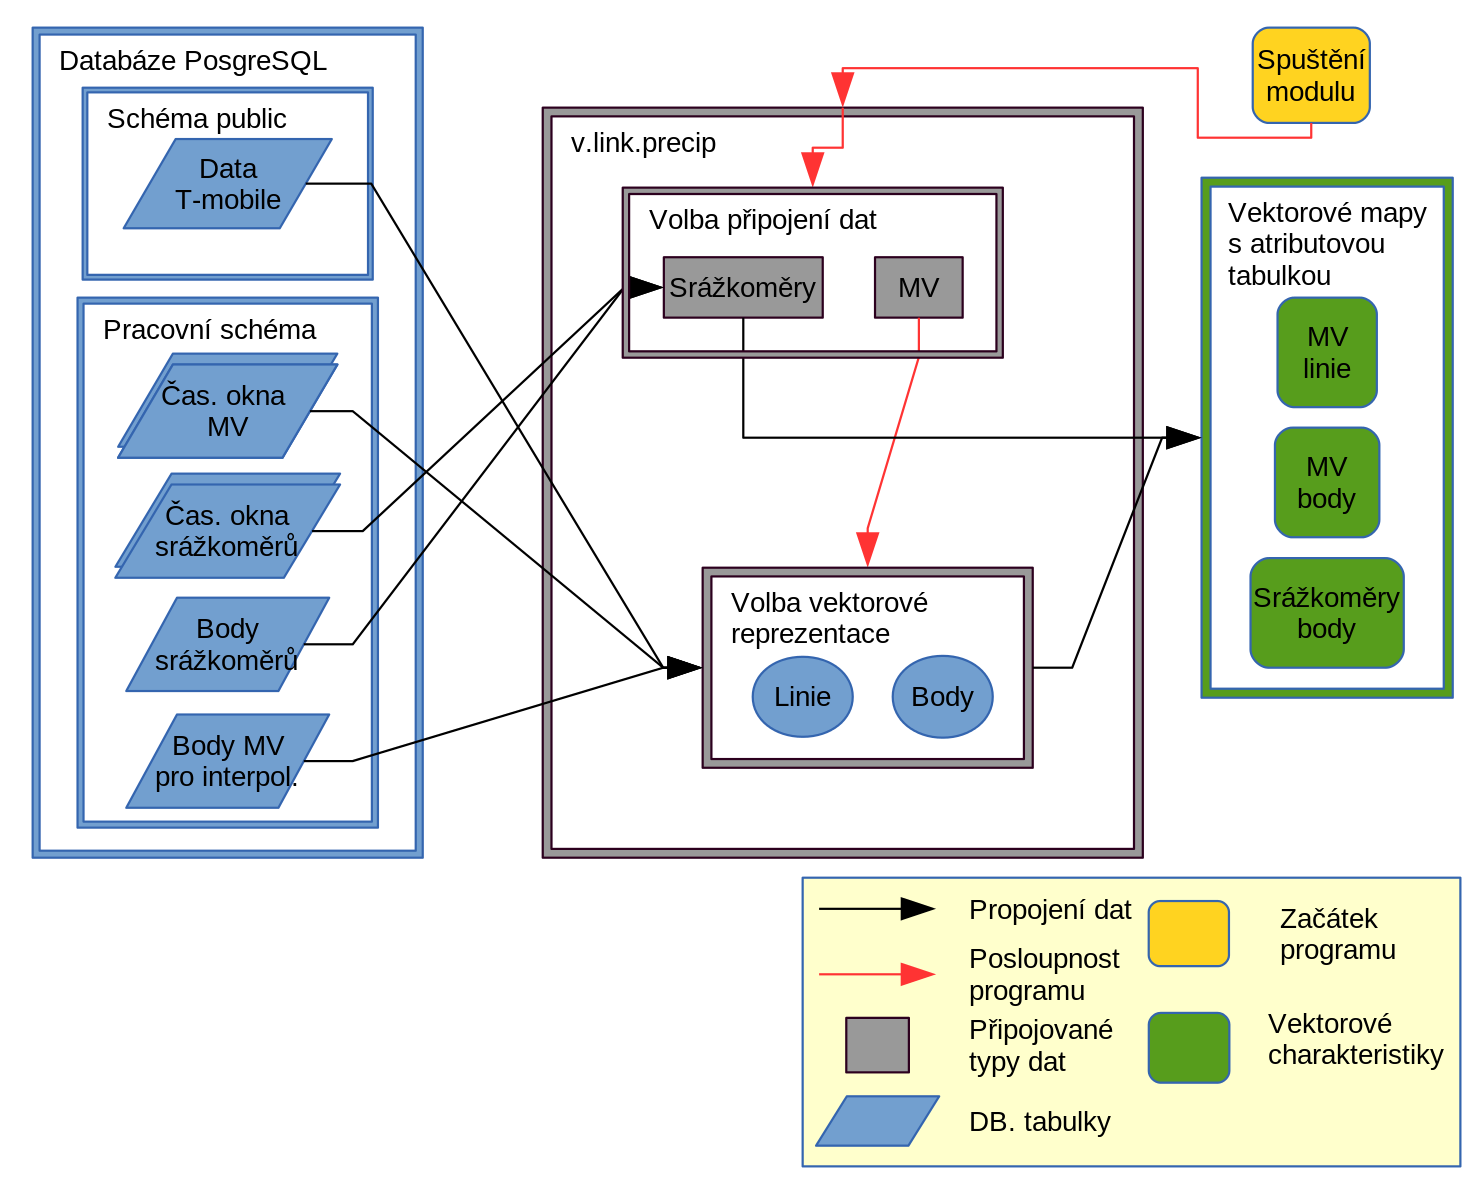
\includegraphics[width=1\textwidth]{./img/grass/diagram2.png}
    \caption[GUI modul]{Schéma připojení vektorových vrstev k atributovým tabulkám \centering  }
        \label{fig:baseline1}
 \end{figure}

\subsubsection{Použití modulu}
Modul při prvním spuštění vytvoří vektorovou vrstvu v nativním
formátu GRASS na základě vytvořené geometrie v databázi
PostgreSQL. K ní připojí zvolenou ta\-bulku reprezentující \uv{časové
okno}. Při dalším připojení jiného \uv{časového okna} je původně připojená
tabulka odpojena a k té samé vektorové vrstvě se připojí tabulka nová. Modul
je tvořen dvěma GUI záložkami \textit{Required} a \textit{Optional}.

\paragraph{Záložka Required} obsahuje pouze povinné parametry.
Parametr \texttt{schema} označuje pracovní schéma, ve kterém jsou
uloženy výsledky pro zobrazení. Parametr \texttt{type} nastavuje, zda chceme
připojovat  hodnoty ke srážkoměrům nebo k MV spojům.
Při volbě MV spojů je možné určit, zda chceme připojit hodnoty k 
vektorové mapě v podobě spojů či bodů (body z interpolace). 
Možnosti konfigurace jsou znázorněny ve schématu \ref{fig:baseline1}



\paragraph{Záložka Optional}  obsahuje přepínače a parametry:
\begin{description}
\item[-c] slouží pro případ, kdy bude nutno pracovat s více \uv{časovými
  okny} najednou. Přepínač \texttt{-c} \uv{časová okna} nepřipojuje k
  vektorové vrstvě \textit{"link\_nat"}, ale vytváří nové s názvem
  ($"view" + <hodnota timestamp>$). Při této volbě dochází k
  redundanci dat vektorových vrstev.
\item[-a] umožňuje dávkově vytvořit pro všechna \uv{časová okna} z modulu
  \textit{r.mwprecip} vektorové vrstvy s připojenými tabulkami. Tato
  funkce je vhodná k přípravě dat pro časoprostorové analýzy.
\item[-p] vypíše na standardní výstup hodnoty připojené atributové
  tabulky.
\item[-r] vymaže dočasné soubory z pracovního schématu.
\end{description}


Parametr \texttt{layername} nastavuje výchozí vektorovou vrstvu, ke
které chceme při\-pojit výsledky v podobě \uv{časových oken}. Podmínkou je,
že daná vektorová vrstva musí obsahovat identifikátory (linkid). V
praxi zde budou nejčastěji připojovány vrstvy vytvořené v rámci
výpočtu primárního modulu \textit{r.mwprecip}. Ty jsou pojmenovány
\textit{linkpoints} s postfixem hodnoty parametru \texttt{step} (počet
bodů či zvolený rozestup mezi body). Pro připojení liniových vrstev MV spojů je výchozí
název \textit{link}.  Škála barev pro vektorovou vrstvu se nastaví
nastavit parametrem \texttt{color}, kde vstupní hodnota je textový
soubor analogický k formátu škály barev pro plošné interpolace.




\newpage
\setcounter{footnote}{1}
\section{Výstupy modulů a jejich využití}
\label{sec:vystupymoduluavyuziti} 
Následující kapitola částečně vyplynula z testování vytvořených modulů a je rozdělena na dvě podkapitoly:
\begin{itemize}
\item Vizualizace \ref{subsec:vizualuzace} a
\item Temporal GRASS framework \ref{subsec:temporalgrassframe}.
\end{itemize}

V první části je kladen důraz na prostorovou interpolaci srážek, kde jsou demonstrovány interpolační metody.
 Zde není zahrnuta analýza výsledků jednotlivých interpolačních metod.
 Jedná se o ukázku možných vizualizací výsledků s nastíněním problematik plošných interpolací z MV spojů.
 
V druhé části je otestován nově navržený časoprostorový model V GRASS GIS s využitím výsledků z vlastních modulů. 
Jelikož se jedná o poměrně novou část GRASS GIS, která byla doposavad ve fázi vývoje, 
kapitola může posloužit jako forma návodu pro uživatele GRASS. 




\subsection{Vizualizace}
\label{subsec:vizualuzace}
V následujících ukázkách jsou demonstrovány vizualizace datových výstupů z modulu r.mwprecip.
Vizualizace je možné kategorizovat na základě datových charakteristik:

\begin{itemize}
\item vektorové mapy jsou vizualizované pomocí linií a bodů, které vycházejí z vytvořené geometrie v databázi,
\item rastrové mapy zobrazují plošné srážky vycházející z plošných interpolací.
\end{itemize}


\paragraph*{Vektorové mapy} lze vizualizovat na základě široké škály volby parametrů. 
V níže uvedených příkladech bylo využito znázornění bodu pomocí čtverce, který na základě 
zvolené škály barev charakterizuje hodnotu intenzit srážek, ze kterých se provedla interpolace.
Konfigurovat  vizualizaci vektorových vrstev je možno provést s využitím modulu \textit{d.vect} a \textit{v.color}.
 
Ukázky grafických výstupů vektorových map jsou sjednoceny s výstupy plošných interpolací,
 které jsou znázorněny v podkapitole (Plošná interpretace srážek).

\paragraph*{Rastrové mapy} v případě výstupů modulu \textit{m.rwprecip} reprezentují
 plošná srážková data, která jsou odhadem
interpolačních metod. K vizualizaci je vytvořena škála barev
odvozená od stupnice používané k radarové odrazivosti srážkových
intenzit.  Škálu barev je možno zvolit jak z předdefinovaných možností, tak z vlastní konfigurace. 
K nastavení škály barev rastrů slouží modul \textit{r.color} .

K vhodné vizualizaci rastrových map lze využít modul \textit{g.gui.animation},
který umožňuje vytvářet animace z po sobě jdoucích rastrů. 

Součástí další kapitoly jsou obrázky reprezentující ukázky vizualizovaných rastrových map.

\subsubsection{Plošná interpretace srážek}
Na níže uvedené plošné interpolace nenavazují rozsáhlé analýzy jejich přesností,
 ale primárně poukazují na novou problematiku interpolačních
metod, která definuje možný směr dalších výzkumů. 
V textu jsou pouze rozebrány základní charakteristiky 
interpolací v GRASS GIS a jejich typické vlastnosti.
  

Výsledek plošných interpolací je ovlivněn mnoha faktory, které se
podílejí na správnosti interpolovaných hodnot. Interpolace z
liniových vektorů je obecně v GIS neobvyklá a jediným východiskem pro
využití podporovaných interpolačních metod v GRASS je nahrazení
liniové reprezentace body. K tomto účelu byly do  modulu \textit{r.mwprecip} přidány
 funkce pro interpolaci bodů podél MV spojů.

MV spoje jsou poměrně hustě rozmístěny a z toho plyne velká
variabilita v možném rozložení a volbě počtu bodů. Z ukázek
interpolací je patrné, že počet bodů vstupujících do interpolací má
velký vliv na jejich výsledky. Zcela jistě má vliv na výsledek i
dostupný vzorek dat. Ten se skládá ze dvou  uzlů,
které jsou od sebe, při porovnáním s reálnou hustotou rozložení
uzlů, velmi vzdálené. Při využití disponibilních vysílačů, např.
sítí T-mobile, by prostorovou mezeru doplnilo několik desítek dalších. 
Tím jsou výstupy následujících interpolací oproti
možným výsledkům značně ovlivněny. 


\paragraph*{Rozlišení a region} rastrové mapy nastavuje automaticky
modul \textit{r.mwprecip}. Přepínačem \texttt{-g} lze výchozí
nastavení ignorovat. 


%%% ML: asi by to chtelo vysvetlit, co presne modul dela a hlavne jak
%%% je vypocetni region nastaven...

\begin{figure}[h!]
\begin{footnotesize}
\lstset{extendedchars=false,
escapeinside=''}
\begin{lstlisting}[style=mybash]
# V'ý'choz'í' nastaven'í' modulu r.mwprecip
        grass.run_command('g.region',
                          vect='link',
                          res='00:00:01',
                          n='n+00:00:20',
                          w='w-00:00:20',
                          e='e+00:00:20',
                          s='s-00:00:20')
\end{lstlisting}
\end{footnotesize} 
\end{figure}

%%% MK: vysvetleno
%%% ML: OK
Parametr \texttt{vect} umožňuje nastavení velikosti výpočetního regionu 
na základě území vektorové mapy (MV spojů) ohraničené minimálním obdélníkem.  
Parametr \texttt{res} nastavuje velikost rozlišení výpočetního regionu,
který je možno definovat v délkové nebo stupňové míře a to podle výchozího 
referenčního systému dané lokace. Parametry \texttt{n, s, e, w} určují rozšíření čí zmenšení daného výpočetního regionu ve směrech jednotlivých světových stran.

\subsubsection*{v.surf.bspline}
Modul \textit{v.surf.bspline} má parametr \texttt{method}, který
umožňuje volby bilineární a~bikubické interpolace.

\begin{description}

\item Parametry \texttt{sie} a \texttt{sin}, určují vzdálenost spline
  křivky pro jednotlivé kroky ve směrech východ-západ (sie) a
  sever-jih (sin). Maximální hodnota \texttt{sie} a \texttt{sin}, určuje vzdálenost spline
  křivky pro jednotlivé kroky ve výše uvedených směrech. Pro oba směry by neměla 
  být menší než vzdálenost známých bodů \footnote{\ref{subsec:temporalgrassframe}
}.

\item Parametr \texttt{lambda\_i} (Thykonov regularization parameter)
  ovlivňuje vyhlazení interpolace. Při volbě malé \texttt{lambda\_i}
  jsou interpolované hodnoty více závislé na vstupních hodnotách;
  vysoké \texttt{lambda\_i} vytvoří výsledný rastr \uv{jemnější}. Pro
  optimální zjištění parametru slouží přepínač \texttt{-c}, který pro
  nastavenou délku křivky spline vypočte \acs{RMS} charakteristiky.
\end{description}
%%% MK: zakomentovano na prani martina
\begin{comment}
\begin{figure}[h!]
\begin{footnotesize}
\lstset{extendedchars=false,
escapeinside=''}
\begin{lstlisting}[style=mybash]
Table of results:
v.surf.bspline complete. Cross validation finished \
  sie = 0.010000 and sin = 0.010000
    lambda |       mean |        rms |    
   0.00500 |    -1.6996 |     9.5957 |
   0.01000 |    -1.6824 |     9.5004 |
   0.02000 |    -0.6679 |     9.5563 |
\end{lstlisting}
\end{footnotesize} 
\end{figure}
\vskip-2ex
\end{comment}

\begin{figure}[h!]%
    \centering
    \subfloat[Bikubická interpolace -- nahrazení linie jedním bodem, sie=sin=0.01, lambda\_i=0.05]{ 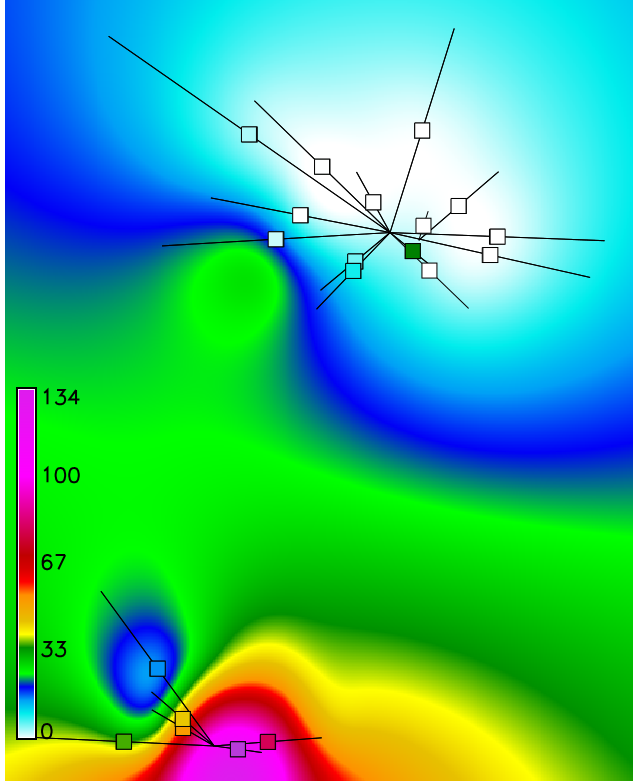
\includegraphics[width=0.33\textwidth]{./img/intanalys/bic1.png} }%
    \qquad
    \subfloat[Bikubická interpolace -- body po 500 m,  sie=sin=0.01, lambda\_i=0.01]{ 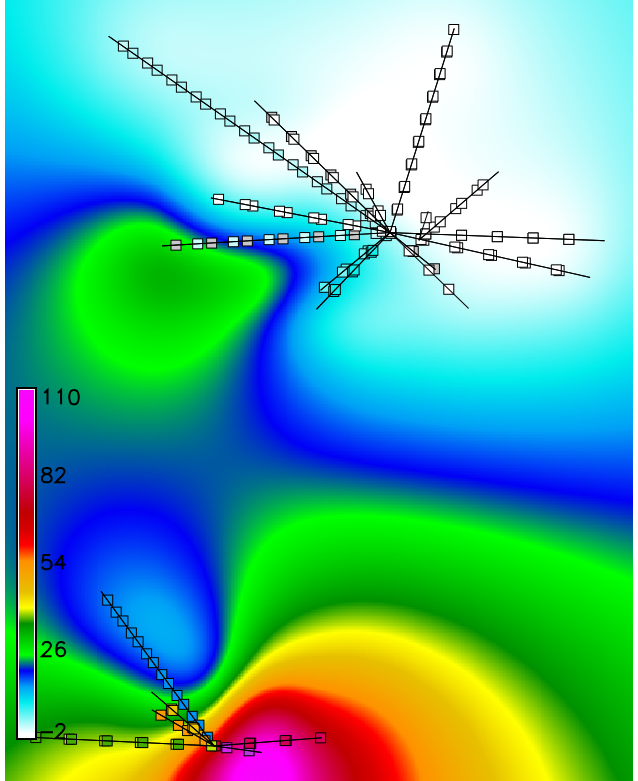
\includegraphics[width=0.33\textwidth]{./img/intanalys/bic500.png} }%
           \caption[Bikubická interpolace]{Názorné porovnání výsledků bikubické interpolace s různou volbou rozložení bodů \centering}%

    \label{fig:example}%
\end{figure}





%%% ML: priste bych legendu daval mimo obrazek (pokud nemas skripty,
%%% ktere obrazky vyrabeji automaticky, tak uz to takto nech byt)
%%% MK: nemam, o moznisti jsi mi rekl az kdyz bylo vse hotove :)
%%% ML: pro priste :-)


\subsubsection*{v.surf.idw}
Modul \texttt{v.surf.idw} umožňuje nastavení exponentu \texttt{power}
a počet známých bodů \texttt{npoints}, ze kterých se odhadovaný bod
určuje \ref{sec:plostneinterpolace}.


Metoda \ac{IDW} v GRASS nedisponuje některými nastaveními, které by byla vhodná
pro odhad plošných srážek pomocí MV. Jedním z nastavení je
podpora rozdělení na sektory, která by byla v tomto případě výhodná
pro rozdělení interpolované mapy na segmenty. Z nich by se do
výpočtu neznámé buňky zahrnoval zvolený počet bodů. Dalším důležitým
omezením u metody IDW je určení vzdálenostní bariéry, která ignoruje vzdálené
body při výpočtu. Z volby možných dvou parametrů vyplynulo několik
poznatků:
\begin{figure}[h!]%
    \centering
    \subfloat[IDW interpolace -- nahrazení linie jedním bodem, npoints=15, power=1.5]{ 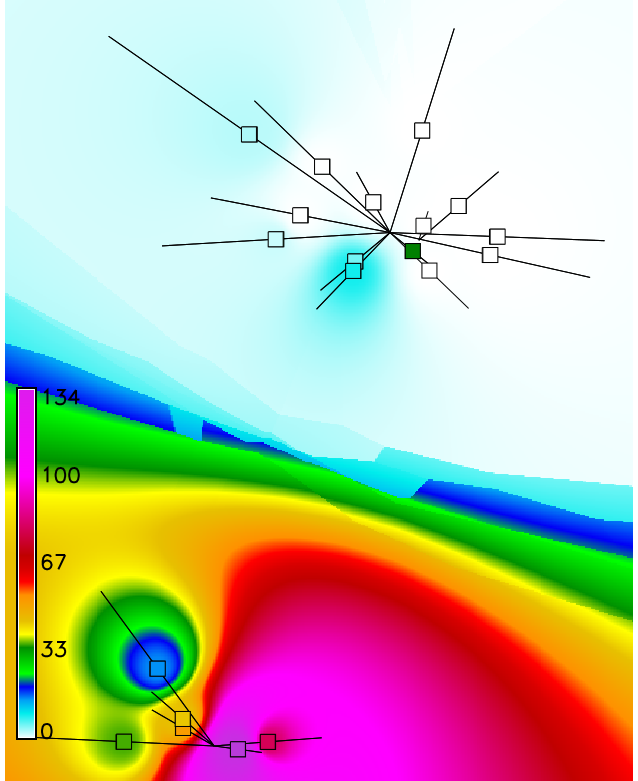
\includegraphics[width=0.33\textwidth]{./img/intanalys/idw1.png} }%
    \qquad
    \subfloat[IDW interpolace -- body po 500~m, npoints=150, power=1.5]{ 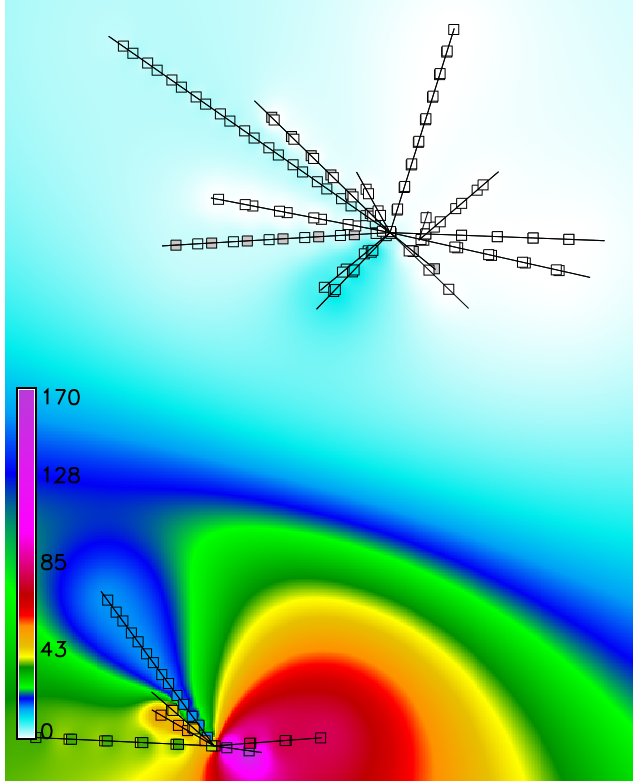
\includegraphics[width=0.33\textwidth]{./img/intanalys/idw500.png} }%
       \caption[Interpolace IDW]{Názorné porovnání výsledků interpolace IDW s různou volbou rozložení bodů \centering}%
	
    \label{fig:idwpic}%
\end{figure}
\begin{description}
\item \textbf{Volba počtu bodů} z nichž se provádí interpolace, má
  velký vliv výsledky. IDW je vhodná interpolační metoda pro
  rovnoměrně rozmístěné známé body. V tomto případě je vhodné
  výpočetní region rozdělit do dvou částí, čímž se do jisté míry
  nahradí chybějící parametr pro maximální vzdálenost. Při takovémto postupu však není 
   simulována reálná situace možných výsledků s využitím plnohodnotného vzorku dat (hustota MV spojů).
  Při plošné interpolaci z dostupného vzorku dat a konfiguraci interpolace viz. obr. \ref{fig:idwpic} a),  je způsobován na pomy\-slné hranici mezi danými lokalitami nespojitý povrch.

\item \textbf{Volba exponentu} ovlivňuje váhu (vzdálenost)
  jednotlivých bodů. Při volbě vysokého exponentu je odhadovaná buňka
  vypočtena s velkou váhou nej\-bližších známých bodů. S přímou
  návazností na volbu exponentu je metoda IDW charakteristická
  tvořením interpolačních artefaktů v podobě koncentrických isolinií,
  které se často nazývají "\textit{bull eyes"}(býčí oči).
\end{description} 



Jednou z možných chyb interpolace IDW je přenesení hodnoty (srážek)
přes mezilehlý známý bod. V praxi pak dochází k tomu, že vysoké
srážkové intenzity ze známého bodu mohou přeskočit oblast se známou
nulovou srážkou a použít ji zcela chybně pro výpočet dané buňky.
Zamezením tohoto jevu se zamezuje pomocí specifické úpravy metody IDW, 
která spočívá v rozdělení oblasti na kvadranty, ze kterých zasahuje do výpočtu  pouze nejbližší bod \cite{krejci}.


%%% ML: rozepsat RST a podobne i IDW, nebo alespon odkaz na seznam
%%% zkratek
%%% MK: doplneno na pri prvnim zmineni
%%% ML: mozna doplit zkratky (\arc)?

%%% ML: v textu by mely byt odkazy na obrazky, to pomuze predevsim
%%% kdyz obrazek pretece na dalsi stranku
\begin{figure}[h!]%
    \centering
    \subfloat[RST interpolace -- nahrazení linie jedním bodem, tension $=30$]{ 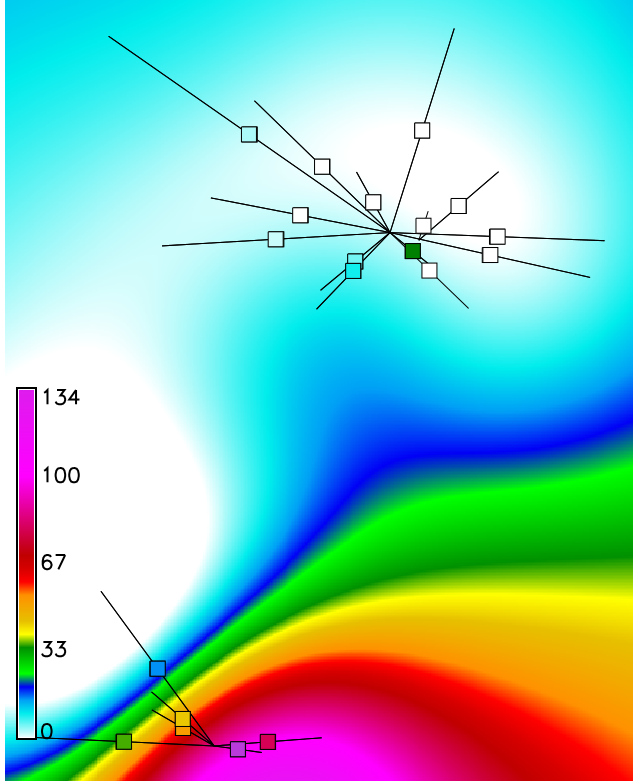
\includegraphics[width=0.33\textwidth]{./img/intanalys/rst1.png} }%
    \qquad
    \subfloat[RST interpolace -- body po 500~m, tension $=20$]{ 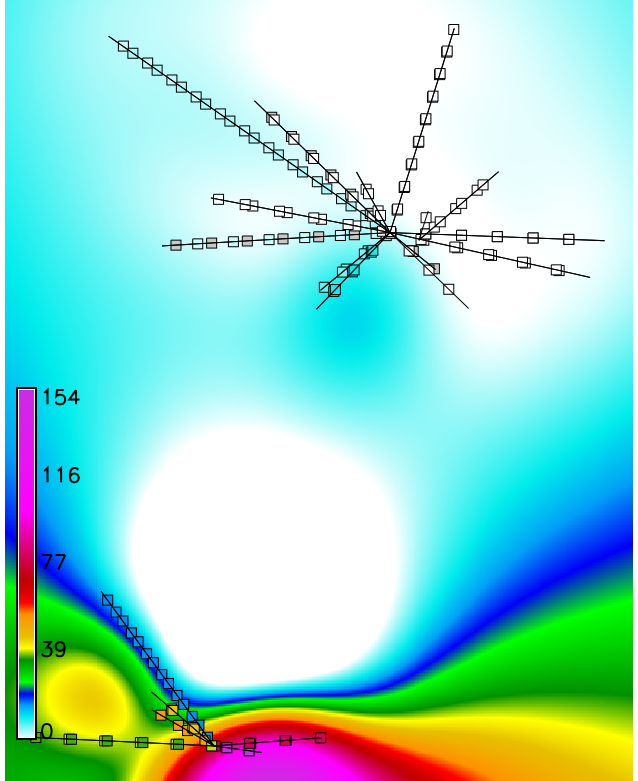
\includegraphics[width=0.33\textwidth]{./img/intanalys/rst500.png} }%
    \caption[Interpolace RST]{Názorné porovnání  výsledků interpolace RST s různou volbou rozložení bodů \centering}%
    \label{fig:rst}%
\end{figure}
\subsubsection*{v.surf.rst}
Metoda \ac{RST} odhaduje neznámé hodnoty pomocí spline křivky, která 
je definována jako funkce procházející měřenými body a má minimální
 křivost. Z toho mimo jiné plyne, že interpolované hodnoty mohou nabývat 
 hodnot mimo interval hodnot známých, což má za důsledek, že při interpolaci
  srážek mohou vznikat srážky záporné.


Metodu RST představuje v GRASS modul \textit{v.surf.rst}. Mimo výškové mapy
 povrchu generuje jiné  specifické rastry vyplývající z generovaného povrchu: 
 mapu sklonu, orientace, zakřivení a
dalších. Dále umožňuje volbu maximální a minimální vzdálenosti bodů
při segmentaci. Mezi charakteristické parametry této metody patří:
\texttt{dmin} a \texttt{dmax} umožňující nastavení minimální a
maximální vzdálenosti mezi body; parametr \texttt{tension} určující
napětí povrchu. Obrázek \ref{fig:rst} znázorňuje dva výsledné rastry s 
rozdílnou konfigurací bodů a nastavením tenze.



%%% ML: zde bych umele zvetsil mezeru (nestatne strankovani), pokud
%%% dojde k pohybu v textu, tak je nutno opravit

\vskip 3\baselineskip

%%% ML: melo by zde vic odkazu na teoretickou cast (viz kap. \ref{xx})
%%% a pod.

%%% ML: dataset by sel spravne psat jako datova sada, ale klidno to
%%% tak nech (je to detail)

\subsection{Temporal GRASS framework}
\label{subsec:temporalgrassframe}

Kapitola je zaměřena na možné využití \textit{Temporal GRASS framework} (TGRASS)
%%% ML: prilis dlouhe souveti...
%%% MK: Rozdeleno
%%% ML: mirne preformulovano...
pro analýzu výsledků z modulu \textit{r.mwprecip}.  Protože je
TGRASS poměrně nový a~v~současné době existuje jen několik málo nastínění jeho
možné aplikace, bude následující text částečně psán stylem podobným
formě návodu. Tato forma je zvolena z důvodu, aby mohl text
 sloužit jako úvod pro experimentální využití
modulu v GRASS GIS v rámci problematiky MV spojů. Tento směr má
logickou návaznost na zadání projektu.

Pro názornost bylo využito výstupů z modulu \textit{r.mwprecip} ve
zvoleném časovém intervalu tří dnů. Jednotlivá \uv{časová okna} byla
vygenerována v časovém kroku 1~minuta.  Rastrové mapy byly
interpolovány metodou RST a IDW pomocí jednoho bodu uprostřed linie
(\texttt{pmethod=count, step=1}).



\subsubsection{Základní operace}

\paragraph*{Volba databáze} pro správu časoprostorových má dvě možnosti: databáze  SQLite (nativní v GRASS), která je
nastavena jako výchozí nebo modulem \textit{t.connect} definovat
připojení k externí databázi PostgreSQL.

%%% ML: misto casoveho bych spise psal casoprostroveho datasetu...
%%% MK: ok
\paragraph*{Vytvoření } časoprostorového datasetu je prvním nezbytným
krokem a slouží k němu modul \textit{t.create}, např:
\footnote{\url{http://grass.osgeo.org/grass70/manuals/t.create.html}}.
\begin{figure}[h!]
\begin{footnotesize}
\lstset{extendedchars=false,
escapeinside=''}
\begin{lstlisting}[style=mybash]
t.create output=temporalLetnany title="MV letnany" \
         description="ukazka vytvoreni datasetu"                        
\end{lstlisting}
\end{footnotesize} 
\end{figure}
\vskip-2ex
\paragraph*{Registrace} jednotlivých map do datasetu je druhým nutným
krokem. Modul \textit{r.mwprecip} do pracovní složky automaticky
generuje soubor vhodný pro tuto registraci (ve formátu "$<$název
mapy$>$ $<$separátor$>$ $<$časová známka$>$").

\begin{figure}[h!]
\begin{footnotesize}
\lstset{extendedchars=false,
escapeinside=''}
\begin{lstlisting}[style=mybash]
temp14.lview2013_09_11_23_19_rst|2013-09-11 23:19:00                       
\end{lstlisting}
\end{footnotesize} 
\end{figure}
\vskip-2ex
Registraci map do časového datasetu umožňuje modul \textit{t.register}
\begin{figure}[h!]
\begin{footnotesize}
\lstset{extendedchars=false,
escapeinside=''}
\begin{lstlisting}[style=mybash]
t.register input=temporalLetnany file=/adresar/tmp_temp14/ \
           timewin_l_2013-09-08_23:59:00|2013-09-11_23:59:00        
\end{lstlisting}
\end{footnotesize} 
\end{figure}
\vskip-2ex

Pro kontrolu úspěšné registrace je možné využít modul \textit{t.info}.
\begin{figure}[h!]
\begin{footnotesize}
\lstset{extendedchars=false,
escapeinside=''}
\begin{lstlisting}[style=mybash]
t.info input=temporalLetnany      
\end{lstlisting}
\end{footnotesize} 
\end{figure}
\vskip-2ex
Po spuštění se vypíše tabulka s obecnými informacemi o časovém
datasetu. Jednou s užitečných funkcí je vypsání celé historie příkazů
v daném datasetu. Vypíše se přepínačem \texttt{-h}.

Další fází je kontrola topologie časového datasetu a provádí ji modul
\textit{t.topology}.

\paragraph*{Odstranění a kontrola} patří mezi podstatné základní
operace při práci s časo\-prostorovým datasetem.
\begin{description}
\item[t.remove] smaže celý časoprostorový dataset.  
\item[t.rename] umožňuje  přejmenování datasetu.
\item[t.unregister] odstraní zvolené připojené mapy z datasetu
\item[t.support] umožňuje úpravy metadat
\end{description}


\paragraph*{Vytvoření sub datasetu} zle v případě, že již jeden
časový dataset existuje. Mohou nastat dva případy, kdy je vhodné
využít modul \textit{t.rast.extract}.

První je situace, kdy jsou z modulu \textit{r.mwprecip} vygenerována
\uv{časová okna} z~většího časového intervalu, než chceme využít k analýzám
TGRASS. V takovém případě je možné při registraci interaktivně
editovat registrační soubor, nebo využít \textit{t.rast.extract} a
definovat v parametru \texttt{where} podmínku, která vymezí časová rozsah nového datasetu.

Modul mimo jiné podporuje mapový kalkulátor, kde parametr
\texttt{expression} umožňuje pomocí mapové algebry definovat nahrazení
jednotlivých buněk jinými.
\begin{figure}[h!]
\begin{footnotesize}
\lstset{extendedchars=false,
escapeinside=''}
\begin{lstlisting}[style=mybash]
t.rast.extract input=temporalLetnany where="start_time > \ 
    2013-09-10 23:59:00"output=selected_precip base=new_prec_map \
    expression="if(precipitation < 0, null(), precipitation)" 
\end{lstlisting}
\end{footnotesize} 
\end{figure}
\vskip-2ex
Ve tomto případě jsou nahrazeny hodnoty menší než 0 (MV šum - chyby)
hodnotou NULL. To je výhodné například pro vizualizaci srážek nad
podkladovou mapou, kde je vodné, aby nulové hodnoty byly průhledné.

\paragraph*{Export} časoprostorových datasetů např. pro zálohování či
přenesení na jiné úložné médium se provede pomocí modulu
\textit{t.rast.export} pro rastrové datasety \newline a \textit{t.vect.export}
pro vektorové datasety.

Modul \textit{t.rast.out.vtk} umí exportovat rastry do textové formy
\textit{VTK DataFile Version 3.0}. Export tímto modulem je možnost,
jak dávkově exportovat data z modulu \textit{r.mwprecip}.

Atributovou tabulku časoprostorového datasetu lze vypsat modulem
\textit{t.vect.db.select}. Volbou oddělovače jednotlivých
sloupců (\texttt{separator}), lze např. uzpůsobit výstup do formátu \ac{CSV}.


%%% ML: v odstavci chybi odkaz na obrazek (viz obr.~\ref{x}), tak jako
%%% vsude v textu...
%%% MK: doplneno
%%% ML: doplnena mezera, jinak OK
\paragraph*{Zobrazení časoprostorových datasetů } umožňuje modul
\emph{g.gui.timeline} \ref{fig:timeline}, který na časové ose zobrazuje zvolené
časoprostorové datasety a jejich granularitu. Modul dokáže zobrazit jak
časovou osu ve 2D, tak časovou krychli ve 3D.

\begin{figure}[h!]
    \centering
    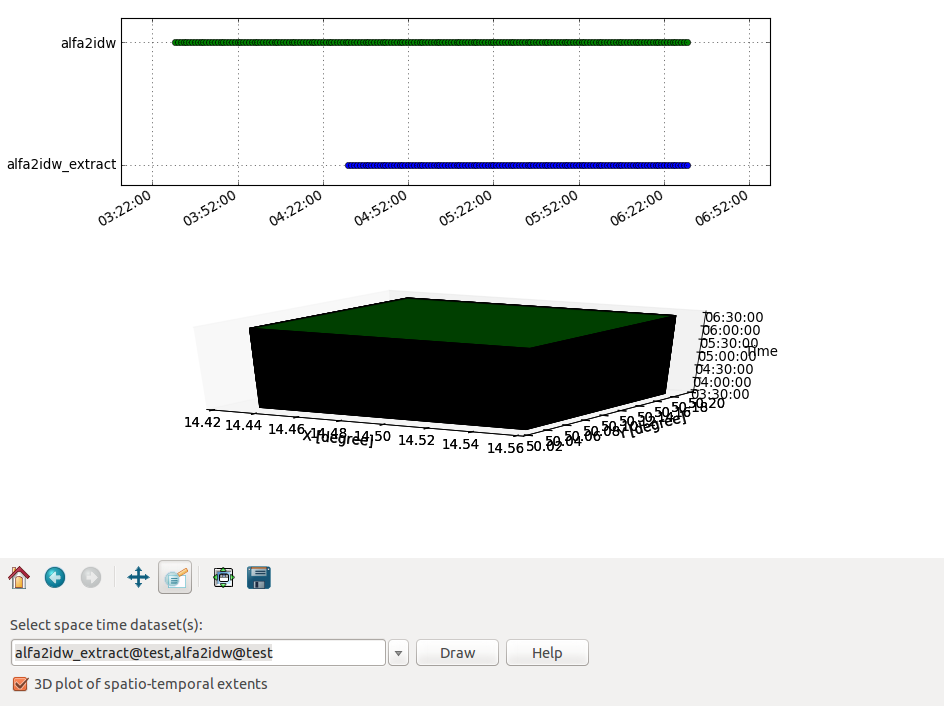
\includegraphics[width=0.7\textwidth]{./img/temporal/timeline.png}
    \caption[Timeline]{\centering  Modul \textit{g.gui.timeline} pro grafický náhled časových datasetů}
    \label{fig:timeline}
 \end{figure}  




 \paragraph*{Vytvoření intervalů} Při registraci map jsou časové
 známky registrovány jako absolutní bod v čase. Pro některé analýzy
 je třeba pracovat s časovými intervaly. Modul \textit{t.snap} vytvoří
 automaticky intervaly podle granularity datasetu.
%%% ML: tohle bych vynechal
% Modul nemá kromě
%  \texttt{input} a \texttt{type} žádné další parametry.
%%% MK: ok



 \paragraph*{Posunutí časového datasetu} Posunutí časového datasetu v
 čase může být využito například při změně času nebo při práci s
 daty s různými časovými referencemi. Modul \textit{t.shift} umožňuje
 posunutí datasetu o absolutní hodnotu.
\begin{figure}[h!]
\begin{footnotesize}
\lstset{extendedchars=false,
escapeinside=''}
\begin{lstlisting}[style=mybash]
t.shift input=rastr@tletnany granularity=1 hours
\end{lstlisting}
\end{footnotesize} 
\end{figure}
\vskip-2ex Tímto příkazem jsem  posunuli časový dataset o 1 hodinu dopředu.



%%% ML: nepsal bych jake ma modul parametry, ale co dela...
%%% MK: ok
\paragraph*{t.merge} je modul, který umožňuje spojení dvou časových datasetů. 
K nastavení slouží  dva parametry -
\texttt{inputs}, do něhož vstupuje libovolné množství datasetů, které
mají být spojeny v jeden \texttt{output}. Podmínkou je, že spojované
datasety musí být stejného časového typu (absolutní nebo relativní).


\subsubsection{Základní analýzy}
\label{subsubsec:casoprostoranal} 


\paragraph{Agregační funkce} slučují buňky o stejných rastrových
souřadnicích do jednoho rastru na základě zvolené matematické funkce
(průměr, suma, max, min atd.). Rastry jsou slučovány podle zvoleného
časového kroku.

Modul, který implementuje agregační funkci, se jmenuje
{\it t.rast.aggregate} 

V příkladě uvedeném níže byly pomocí agregační funkce vytvořeny rastry
reprezentující sumy srážkových intenzit po 15 minutách. Vytvořený
dataset je nazván \emph{temporalLetnany}.
\begin{figure}[h!]
\begin{footnotesize}
\lstset{extendedchars=false,
escapeinside=''}
\begin{lstlisting}[style=mybash]
t.rast.aggregate input=temporalLetnany output=temporal_aggreg \
       basename=sum15minute granularity=15 minutes method=sum
\end{lstlisting}
\end{footnotesize} 
\end{figure}
\vskip-2ex
Jinou agregační funkcí je \textit{t.rast.aggregate.ds}, která má na
vstupu dva datasety \emph{a} a \emph{b}. Agregací
 datasetu \emph{a} podle datasetu \emph{b}, tedy vytvoření
časové topologie \emph{a} podle předlohy \emph{b}.

Další možností je modul \textit{r.rast.series}, který využívá k agregaci jiných
algoritmů a je určen pro analýzu celého datasetu bez zvolené
granularity.  Příkladem je vytvoření rastru s maximálními intenzitami
srážek v celém časovém intervalu datasetu. Byly vytvořeny maximální
intenzity časového datasetu z plošných interpolací \ref{fig:maximasraz} RST a IDW.


\begin{figure}[h!]
\begin{footnotesize}
\lstset{extendedchars=false,
escapeinside=''}
\begin{lstlisting}[style=mybash]
t.rast.series input=idwt method=maximum output=idwt_seriesmax           
t.rast.series input=rstt method=maximum output=rstt_seriesmax    
\end{lstlisting}
\end{footnotesize} 
\end{figure}
\vskip-2ex
%%% ML: obrazek jsem zvetsil na standardni velikost
\begin{figure}[h!]%
    \centering
    \subfloat[RST]{ 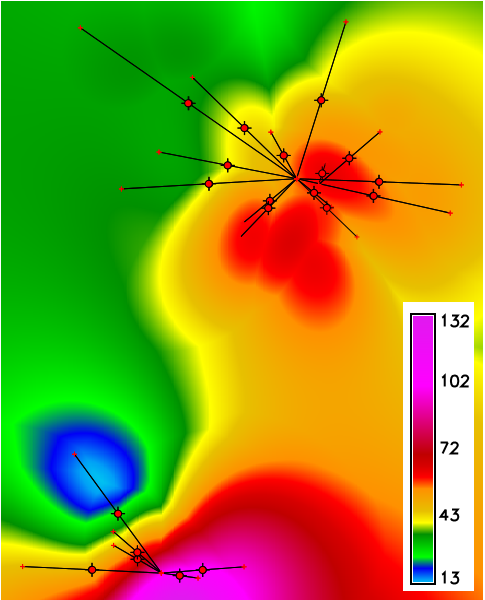
\includegraphics[width=0.33\textwidth]{./img/intanalys/max1.png} }%
    \qquad
    \subfloat[IDW]{ 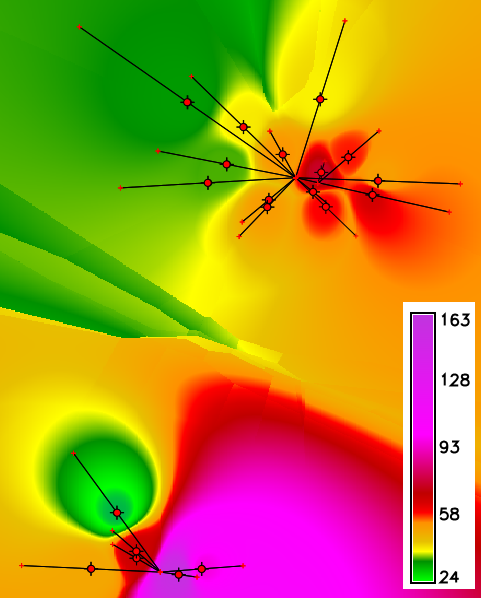
\includegraphics[width=0.33\textwidth]{./img/intanalys/max2.png} }%

    \caption[Serie max]{ Srážková maxima z celého časoprostorového datasetu  \centering }
    \label{fig:maximasraz}
\end{figure}


\newpage

\paragraph*{Mapová algebra} se v rámci TGRASS dělí na dva typy:
\begin{description}
\item [t.rast.mapcalc] plně podporuje funkčnost mapové algebry \textit{r.mapcalc}. Z časo\-prostorového modelu podporuje například start\_time, end\_time, které jsou nejčastěji využívané.
\item [t.rast.mapcalc2] umožňuje využívat časoprostorové algebry, která je v současně dostupných GIS nástrojích první svého druhu.\footnote{Modul nebyl oficiálně představen. Zdroj informace pochází z nepublikovaných materiálů autora (Soren Gebbert)} 
\end{description}

Použití \textit{t.rast.mapcalc} je analogické pro klasickou mapovou
algebru v systému GRASS s rozdílem, že do výpočtu nevstupují jednotlivé
rastry, ale časoprostorové datasety.



\paragraph{Statistické informace } jednotlivých rastrů v časovém
datasetu lze vypsat pomocí modulu \textit{t.rast.univar}. Modul vypíše
po jednotlivých řádcích pro dané rastry jejich základní statistické
charakteristiky. Pro výpis ve formátu s hlavičkou charakterizující
dané hodnoty je možné využít přepínač \texttt{-h}.

\begin{figure}[h!]
\begin{footnotesize}
\lstset{extendedchars=false,
escapeinside=''}
\begin{lstlisting}[style=mybash]
id|start|end|mean|min|max|mean_of_abs|stddev|variance|coeff_var| \
sum|null_cells|cells|first_quartile|median|third_quartile|percentil

alfa1.lview2013_09_09_00_01_rst@test4|2013-09-09 00:01:00 \
|None|0|0|0|0|0|0|-nan|0|0|242109|0|0|0|0
    
\end{lstlisting}
\end{footnotesize} 
\end{figure}
\vskip-2ex

\paragraph{Observace}
Modul \textit{t.vect.observe.strds} umožňuje definovat vektorovou
bodovou vrstvu jako observační objekt. Jednotlivé body této vrstvy pak
zaznamenávají informaci o hodnotě rastru. Prakticky se v databázi
vytváří pro každý rastr ze zvoleného datasetu jedna tabulka. Výsledkem
z observace je nový časoprostorový vektorový dataset.

Při volbě observačních bodů v místech dostupných referenčních
srážkoměrů je umožněno z výsledků observace porovnat interpolované body s
referenčními hodnotami. Vektorovou vrstvu lze zvolit buď z databázové tabulky srážkoměrů nebo
přidat jednotlivé body s využitím modulu \textit{v.in.ascii}.
\begin{figure}[h!]
\begin{footnotesize}
\lstset{extendedchars=false,
escapeinside=''}
\begin{lstlisting}[style=mybash]
# P'ř'id'á'n'í' vektorov'é' bodov'é' vrstvy
v.in.ascii input=
  1|50.152761|14.506575
  2|50.141651|14.519106
  3|50.133124|14.501339
  
  output=srazkomery 
  columns="id text,y double precision,x double precision"
  x=3 y=2
  
# Nasaven'í' observace  
t.vect.observe.strds input=srazkomery strds=idw_gama \
  output=observace vector_output=observace_vec columns=precip
  
\end{lstlisting}
\end{footnotesize} 
\end{figure}


Ve zvolené výchozí databázi se vytvoří \uv{časová okna} v časovém kroku
 granularity datasetu.  Z dané observace je možné výsledky prohlížet v databázi nebo využít modul
 \textit{t.vect.select}, který vypíše tabulku do řádku s hlavičkami a
 oddělovačem podle nastavení parametru \texttt{separator}. Je tedy
 možné například vytvořit standardizovaný výstup formátu CSV.
 
\begin{figure}[h!]
    \centering
    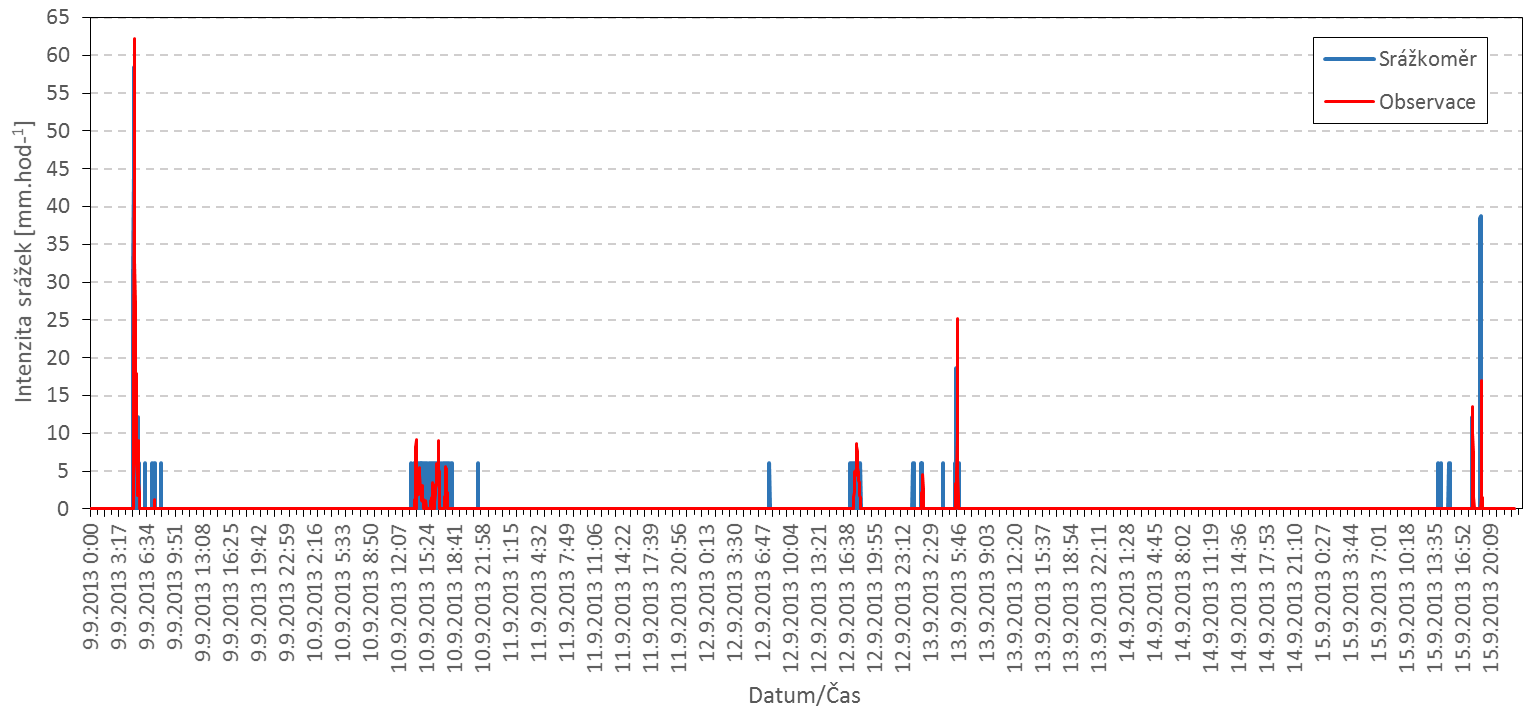
\includegraphics[width=\textwidth]{./img/temporal/grafobs.png}
    \caption[Timeline]{\centering  Porovnání měření srážkoměru s observací rastrového datasetu}
 \end{figure}  




 Modul \textit{t.vect.observe} v současné době nemá zcela vyladěnou
 správu    \acs{RAM}. Při větších počtech vstupních rastrů se data
 ukládají do virtuální paměti a rychlost procesu se
 zpomalí \footnote{Při observaci rastru rozsahu jednoho týdne o časovém
   kroku 1 minuta (cca 10000 rastrů) trval výpočet 17 hodin a zabral
   10 GB virtuální paměti (Ubuntu 13, AMD X3).}. Řešením je rozdělení
 dataset na menší části (\textit{t.rast.extract}).


\subsubsection{Kombinace TGRASS a GRASS}

\paragraph*{Suma z plošných interpolací}
Modulem \emph{r.mwprecip} jsou vygenerována minutová \uv{časová okna} z
jednoho dne. Z oken jsou dále interpolovány plošné srážkové intenzity
metodou RST a IDW. Cílem analýzy je vytvořit rastr, který by
charakterizoval srážkové úhrny z intervalu 3 hodin. 
Odečtením rastrů od sebe je získán objem vody, který představuje objemovou odchylku pro dané dva rastry ve zvoleném časovém intervalu.




\begin{figure}[h!]
\begin{footnotesize}
\lstset{extendedchars=false,
escapeinside=''}
\begin{lstlisting}[style=mybash]
# Vytvo'ř'en'í' datasetu
t.create output=rst_gama semantictype=mean title=Letnany
t.create output=idw_gama semantictype=mean title=Letnany

# Registrace map 
t.register input=idw_gama@test file=timewin_l_idw
t.register input=rst_gama@test file=timewin_l_rst

# Kontrola
t.info input=rst_gama@test                                                      
t.info input=idw_gama@test

# Vytvo'ř'en'í'  subdataset'ů'
t.rast.extract input=idw_gama@test where=(start_time>2013-09-09\
   03:30:00) and (start_time<'2013-09-09 06:30:00') \
   output=idw_gama_extract
t.rast.extract input=rst_gama@test where=(start_time>2013-09-09\
   03:30:00) and (start_time<'2013-09-09 06:30:00') \
   output=rst_gama_extract

# Suma za 3 hodiny
t.rast.aggregate input=idw_gama_extract@test output=\
   idw_gama_extract_aggbasename=gama3aggidw granularity=3 \
   hours method=sum
t.rast.aggregate input=rst_gama_extract@test output=\
   rst_gama_extract_agg basename=gama3aggrst granularity=3 \
   hours method=sum
# Pr'ů'm'ě'r ze dvou map
t.rast.mapcalc inputs=idw_gama_extract_agg@test,\
   rst_gama_extract_agg@test expression=(idw_gama_extract_agg@test+\
   rst_gama_extract_agg@test)/2 output=gamaSUM basename=gama_sum
\end{lstlisting}
\end{footnotesize} 
\end{figure}


%%% ML: opet nestastne umisteni legendy, mela byt mimo rastr

\begin{figure}[h!]%
    \centering
    \subfloat[RST]{ 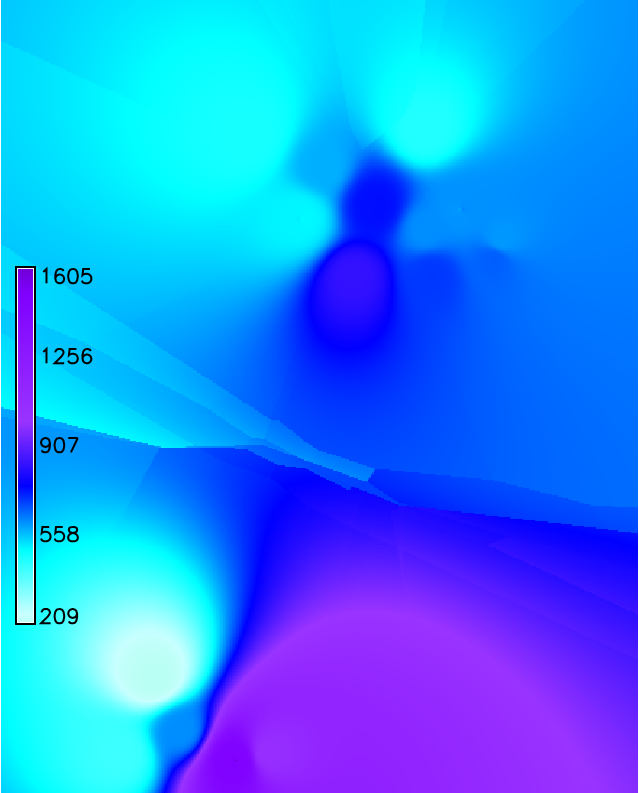
\includegraphics[width=0.19\textwidth]{./img/intanalys/sumrst.png} }%
    \qquad
    \subfloat[IDW]{ 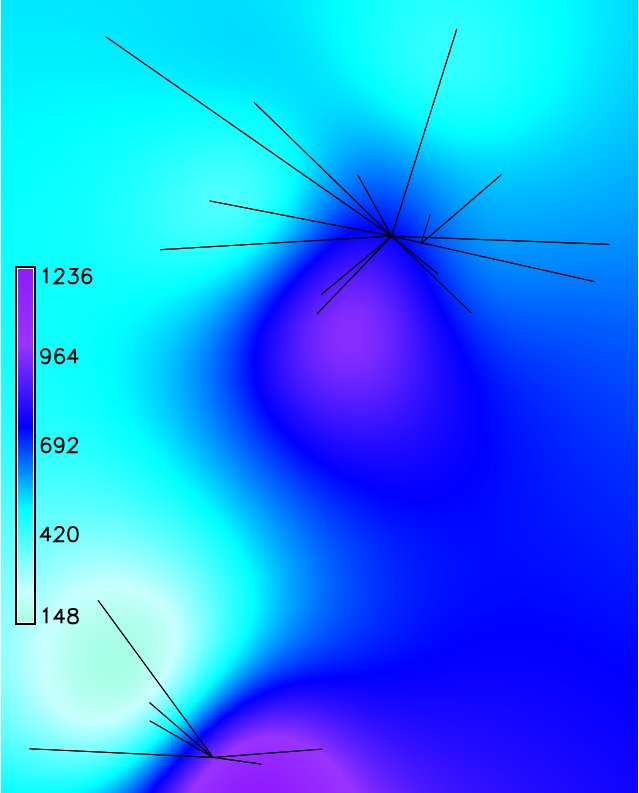
\includegraphics[width=0.19\textwidth]{./img/intanalys/sumidw.png} }%
    \qquad
    \subfloat[Průměr]{ 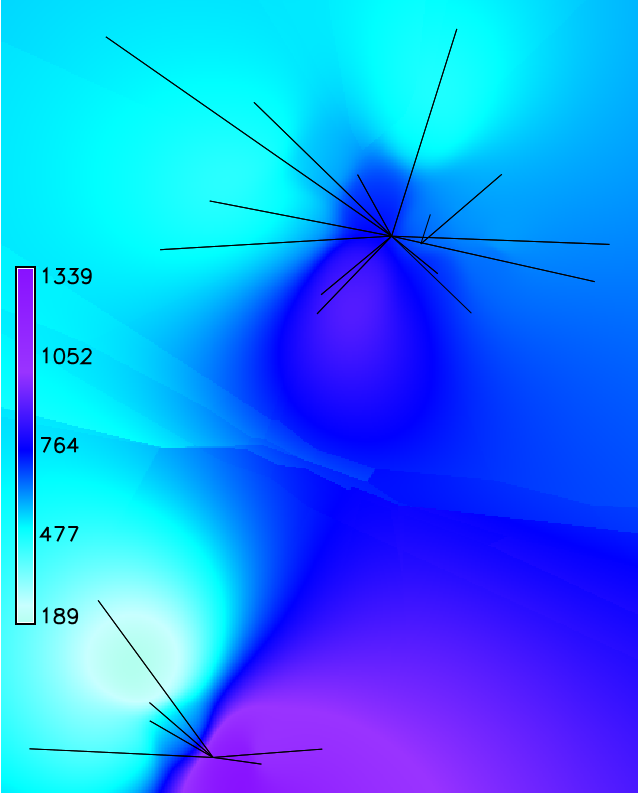
\includegraphics[width=0.19\textwidth]{./img/intanalys/sumavg.png} }%
    \qquad
    \subfloat[Odchylka metod]{ 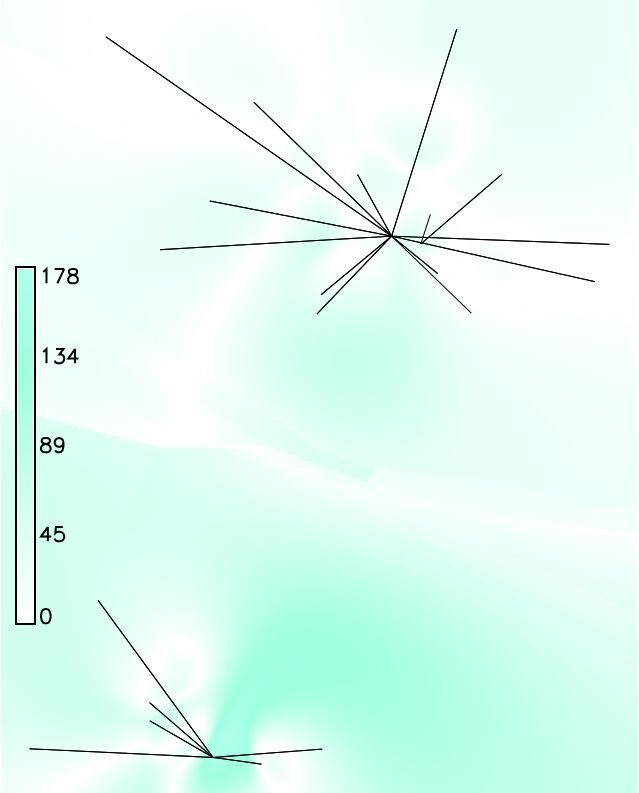
\includegraphics[width=0.19\textwidth]{./img/intanalys/rozdil.png} }%
    \caption[Průměr metod]{ Rastry charakterizující rozdílné výsledky z jednotlivých interpolačních metod\centering}

\end{figure}


Okna z \textit{r.mwprecip} byla v ($mm \cdot h^{-1}$) po jedné minutě,
abychom počítali s~reálnými úhrny, převedeme na ($mm \cdot min^{-1}$).
Pro porovnání obou interpolačních metod je možné v \textit{r.mapcalc}
vytvořit rastr, jehož buňky představují absolutní hodnotou rozdílu
dvou interpolačních metod. Modulem \textit{r.univar} určíme základní
statistické charakteristiky včetně sumy všech buněk rozdílného
rastru. Ta charakterizuje objemovou odchylku dvou rastrů ze tří hodin
v ($mm$) ze zvoleného regionu.

Analýza demonstruje agregaci pouze do jednoho časového okna
(rastru). V~pří\-padě, že bychom chtěli vytvořit agregaci po třech
hodinách z intervalu několika dní, v poslednímu kroku bychom využili
\textit{t.rast.mapcalc} místo \textit{r.mapcalc}.


\paragraph*{Transformace srážek do povodí}
Vytvoření nástroje pro přenesení hrubých dat do formy vypočtených
srážek v GIS prostředí bylo prvním a potřebným krokem k~dalšímu
možnému vývoji dalších GIS nástrojů. Jedním z možných postupů je
automatická klasifikace a transformace srážek do definovaných
subpovodí, která by byla vstupem pro srážko-odtokový hydrologický
model.

%%% ML: otazka - je subpovodi korektni termin?
%%% MK: v literature se to puziva. Jestli je to spatne jsem nenasel. Martin F. toho pouzil v navrhu  moznych BP.
%%% ML: OK
Zjednodušená varianta úlohy demonstruje využití funkcí GRASS a TGRASS
pro transformaci srážek do subpovodí. Postup je následující:

\begin{comment}
\begin{enumerate}
\item {\it r.mwprecip} - vytvoření plošných interpolací
\item TGRASS - {\it t.create}, {\it t.register} a {\it t.rast.aggregate}
\item {\it r.in.gdal} - import   \acs{DMT}
\item {\it r.watershed} -  vytvoření subpovodí z DMT
\item {\it r.volume} - určení objemu vody v subpovodích 
\end{enumerate}
\end{comment}

\begin{enumerate}
\item Prvním krokem je vytvoření plošných interpolací z modulu
  \textit{r.mwprecip}.

\begin{figure}[h!]
\begin{footnotesize}
\lstset{extendedchars=false,
escapeinside=''}
\begin{lstlisting}[style=mybash]
r.mwprecip.py -g database=letnany baseltime=/adresar/norain \
       interval=minute lignore=/adresar/ignore pmethod=count \ 
       step=1 
\end{lstlisting}
\end{footnotesize} 
\end{figure}
\vskip-2ex
Vstupem do parametru \texttt{baseltime} jsou dva časové intervaly
období sucha vyplývající z měření srážkoměrů. Sumy srážek jsou
vytvořeny po 1 minutě. Do parametru \texttt{lignore} vstupuje soubor s
definovanými spoji (linkid), které vykazují vysokou chybovost. Linie
spojů byly nahrazeny vždy jedním bodem, ze kterých se
interpolují hodnoty intenzit srážek pomocí  interpolace RST (výchozí nastavení). Výpočetní
region je nastaven automaticky modulem \textit{r.mwprecip}.


\item Následuje založení časoprostorového datasetu, registrace map a agregace po 15 minutách s funkcí sumace \ref{subsubsec:casoprostoranal}.

\item Modul \textit{r.in.gdal} umožňuje importovat rastrová data většiny obecně známých formátů.  Model terénu ze \ac{SRTM}\footnote{\url{http://edcftp.cr.usgs.gov/pub/data/}} je využit k vytvoření akumulace vody a z té vyplývající jednotlivá povodí v~násle\-dujícím kroku.

\item Modul \textit{r.watershed } umožňuje vytvoření teoretické vodní
  sítě, která je odvozena ze sklonu terénu. Jednotlivé vodní sítě
  představují teoretickou akumulaci vody. Z ní je možné určit
  subpovodí. Tento krok nám umožňuje demonstrovat úlohu bez dostupných
  reálných vektorových vrstev o jednotlivých povodích.


\begin{figure}[h!]
\begin{footnotesize}
\lstset{extendedchars=false,
escapeinside=''}
\begin{lstlisting}[style=mybash]
r.watershed  elevation=dem_srtm threshold=5000 \
          accumulation=accumulation basin=basin
\end{lstlisting}
\end{footnotesize} 
\end{figure}
\vskip-2ex
Parametr \texttt{treshold} určuje jemnost segmentace jednotlivých
povodí. Menší hodnota vede k většímu počtu povodí.
\begin{figure}[h!]%
    \centering
    \subfloat[RST]{ 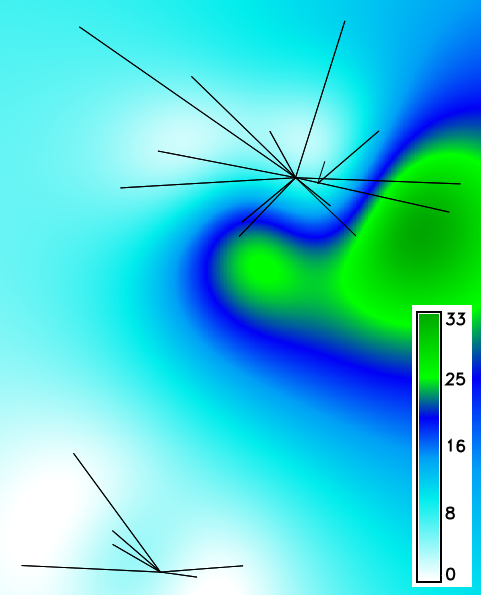
\includegraphics[width=0.33\textwidth]{./img/intanalys/basin1.png} }%
    \qquad
    \subfloat[IDW]{ 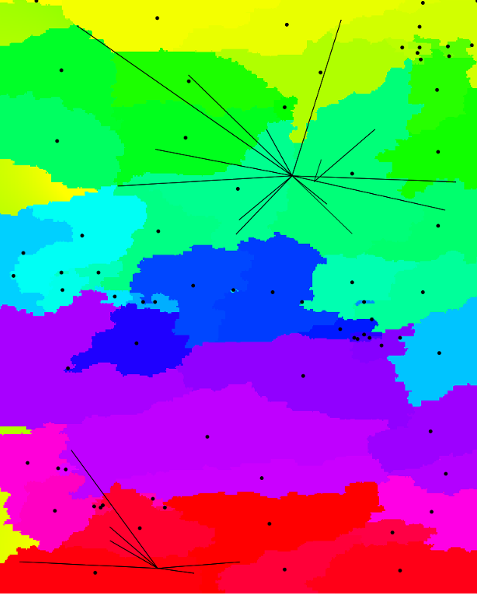
\includegraphics[width=0.33\textwidth]{./img/intanalys/basin2.png} }%
    \caption[GUI modul]{ a) Agregovaný rastr - suma za 15 minut; b) povodí s bodovou vrstvou představující hodnoty jednotlivých povodí.  \centering 
     }
     \label{fig:vysledekaggrrast}
\end{figure}
\item Posledním krokem je určení objemu srážek, které spadly do daných
  povodí. K~tomu je vhodné využít modul \textit{r.volume}, pro který
  jsou vstupními parametry rastr s hodnotami a rastr s klasifikovanými
  územími. Pro vstup rastru s hodnotami je použit výstupní rastr z
  \textit{t.rast.aggregate}. Z názvu \textit{max15minute\_148} nelze
  poznat, o jaký časový interval se jedná; pro získání této informace
  je určen modul \textit{t.rast.list}.
\begin{figure}[h!]
\begin{footnotesize}
\lstset{extendedchars=false,
escapeinside=''}
\begin{lstlisting}[style=mybash]
sum15minute_103	test3  2013-09-10 01:44:00 2013-09-10 01:59:00
\end{lstlisting}
\end{footnotesize} 
\end{figure}
\vskip-2ex

Odtud lze vybrat mapu z požadovaného intervalu, která je vstupem (\texttt{input}) pro \textit{r.volume}. 
\begin{figure}[h!]
\begin{footnotesize}
\lstset{extendedchars=false,
escapeinside=''}
\begin{lstlisting}[style=mybash]
r.volume input=sum15minute_103 clump=basin \
        centroids=volume output=/adresar/r.volumeinfo
\end{lstlisting}
\end{footnotesize} 
\end{figure}
\vskip-2ex


\end{enumerate} 


%%% ML: zvetseno na standardni velikost



Výsledkem je vektorová bodová mapa\ref{fig:vysledekaggrrast}, kde ke každému bodu je připojena
tabulka s hodnotami výsledků (sum, avg). Parametr \texttt{output}
umožňuje uložení ta\-bulky ve formě textového souboru se statistikami
celé plochy výpočetního regionu.  Aby výsledné hodnoty jednotlivých 
povodí byly v jednotkách stejných jako vstupní rastry ($mm \cdot h^{-1}$), 
je nutno výsledný objem vydělit počtem minut, po kterých byla nastavena agregace.

%%% MK: nevim jestli tento odstavec tu ma byt. klidne ho kdyztak smaz
Ve výše zmíněných příkladech byly demonstrovány jednoduché analýzy, které
 sloužily především  k otestování datových výstupů z vlastních modulů a 
 zároveň demonstrovaly základní a pokročilejší funkce časoprostorového modelu TGRASS. 


\setcounter{footnote}{1}
\newpage
\necislovana{Závěr}

Téma zadání "Analýza a vizualizace srážkových dat z mikrovlnných
telekomunikačních spojů pomocí GIS" vycházelo z přímých požadavků
%%% ML: co uvest zadavatele konkretneji (alespon v poznamce pod carou)???
%%% MK:  Jasne
%%% ML: co uvest jeste jeho skolitele???
%%% MK:  jo
zadavatele\footnote{Odpovědný řešitel: Ing. Vojtech Bareš, Ph.D, řešitel: 
 Ing. Martin Fencl: GA ČR 14-22978S \uv{Predikce srážkového odtoku v
  urbanizovaných povodích na základě deštěm generovaného útlumu
  signálu mikrovlnných spojů telekomunikační sítě}} této práce, který spolupracuje na projektu mezinárodního
charakteru. Mezi hlavní požadavky patřilo zpracování naměřených dat do
vhodné formy v prostředí GIS. Tento krok je první a potřebný k dalším
požadavkům vývoje GIS aplikací v rámci problematiky MV
spojů. Sekundárním cílem práce bylo prověřit možné využití
výsledků z vlastních modulů v rámci balíčku časoprostorových funkcí
systému GRASS.

Modul \textit{r.mwprecip} umožňuje výpočet srážek metodou MV spojů z
externí data\-báze, ve které jsou uložena hrubá data z mikrovlnných
vysílačů. Výstupem modulu jsou srážková data ve vhodném formátu  jak pro standardní
funkce GRASS tak pro časoprostorové analýzy. Vypočtená data jsou
dostupná jak ve formě časových oken, tak ve formě vhodné pro export
pro jiná využití. Výstupní formát modu\-lu podporující \textit{Temporal GRASS
  framework} umožňuje větší možnosti při analýze časových řad srážek
včetně dávkového exportu ve vhodném formátu pro vstup do
srážko-odtokových modelů.

%%% ML: uvod a zaver je jedine misto, kde se muze objevit prvni osoba
%%% - prave ze zduvodu zhodnoceni vysledku (to jenom poznamka)

Vývoji vlastních modulů předcházela studia spojená s programovacím
jazykem Python a problematikou databáze PostgreSQL. Kombinace těchto
dvou nástrojů způsobovala problém s optimalizací zápisů do databáze.
Při tisících až desetitisících zápisů do databáze vznikala vysoká
strojová náročnost, která v rámci dostupných funkcí Python knihovny
\textit{psycopg} nešla zcela korektně odstranit. Současná implementace
využívá zápisů do přechodných souborů s následným dávkovým načtením do
databáze.

%%% ML: mozna bych zminit objektovy navrh...
%%% MK doplneno
%%% ML: OK
Prvotní pochopení nároků na daný GIS modul nasvědčovalo výhodě koncipovat 
psaní kódu procedurálně. V závěru psaní aplikace bylo zjištěno, že objektově 
orientovaný návrh by byl vhodnější a to především pro zvyšující se počet funkcí
 modulu. V rámci práce proběhl pokus o objektově orientovaný návrh, 
 který nebyl z časového důvodu dokončen.
%%% ML: take bych zminil publikovani navrzenych modulu v addons (do obhajoby tam budou na 100%)
%%% MK doplneno
%%% ML: OK
Modul \textit{r.mwprecip} je v současné době otevřený doplnění nových
funkcí pro určení baseline a to především pro vývoj nových
metod jejího určování. Moduly, které vznikly v rámci této práce, byly přidány do 
 \textit{GRASS Add-ons} repozitáře 
a jsou současně volně dostupné pro uživatele systému GRASS. 


V rámci vývoje aplikace s využitím \textit{GRASS Python Scripting
  Library} bylo ze vzniklých požadavků na implementaci poukázáno na
možné vylepšení dvou funkcí modulu \textit{v.in.ogr}, které následně
byly vedoucím práce v GRASS GIS upraveny.



Práce ukazuje na možné nové směry výzkumu v oblasti
interpolací srážek z~linio\-vých reprezentací, které jsou zcela novým a
málo zažitým jevem jak na úrovni GIS, tak i  součástí problematiky
rekonstrukce dešťových srážek obecně. S velkou pravděpodobností bude v
nejbližší době ze strany T-Mobile zpřístupněn pro projekt kvalitnější
vzorek dat z pohledu hustoty MV spojů, který by umožňoval výzkum
založený na významnějším datovém podkladu.

%%% ML: teto vete (a celemu odstavci) prilis nerozumim...
%%% MK: jo, nedavalo to smysl. 
%%% ML: OK
Závěrem lze konstatovat, že vlastní modul pro systém GRASS GIS
dostatečně prokázal v rámci testování svou funkčnost a splnil
předpoklad vytvoření datového rozhraní pro standardní a časoprostorové analýzy v prostředí GIS.




















\pagenumbering{gobble}
\newpage
\necislovana{Seznam použitých zkratek}
\begin{acronym}
 \setlength{\parskip}{0ex}
 \setlength{\itemsep}{1ex}
 	\acro{ANSI}{American National Standards Institute}
  	\acro{API}{Application Programming Interface}
  	\acro{CSV}{Comma Separated Values}
  	
  	\acro{DML}{Data Manipulate on Language}
  	\acro{DSD}{Drop Size Distribution}
  	\acro{DPZ}{Dálkový Průzkum Země}
  	\acro{DDL}{Data Definition Language}
  	\acro{DMT}{Digitalní Model Terénu}
  	\acro{EPSG}{Geodetic Parameter Set}	
  	
  	\acro{GIS}{Geographic Information System (Geografický informační systém)}
  	\acro{GNU GPL}{GNU General Public License (Všeobecná veřejná licence GNU)} 
	\acro{GRASS}{Geographical Resources Analysis Support System}
	\acro{GUI}{Graphical User Interface (Grafické uživatelské rozhraní)}
		
	\acro{HMM}{Hidden Markov Model} 
	\acro{IDW}{Inverse Distance Weighting} 
	
	\acro{ITU}{International Telecommunication Union}
	
	\acro{MV}{mikrovlnny}
	\acro{OGC}{Open Geospatial Consortium}
	\acro{OSGeo}{Open Source Geospatial Foundation} 
	\acro{ORDBMS}{Object-Relational Database Management System}
	\acro{RAM}{Random Access Memory (operační paměť)}
	\acro{RGB}{Red Green Blue}
	\acro{RST}{Regular Spline with Tension}
	\acro{RMS}{Root Mean Square}

  	\acro{RSL}{Received Signal Level}
  	\acro{STC}{The Space-Time Composite Data Model}
  	\acro{SRTM}{Shuttle Radar Topography Mission}
    \acro{SRID}{Spatial Reference System Identifier}
    \acro{SQL}{Structured Query Language}
    \acro{TGRASS}{Temporal GRASS Framework}
	\acro{wxGUI}{WxPython-based GUI for GRASS}	
	
	\acro{WKT}{Well-known text}
\end{acronym}





\newpage
\renewcommand\baselinestretch{1.2}
\selectfont
\renewcommand{\refname}{Použité zdroje}
\phantomsection
\addcontentsline{toc}{section}{\refname}

\begin{thebibliography}{99}
\label{literatura}




%\bibitem{radar_meterology}
%RAGHAVAN, S. \textit {Radar meteorology}.
%31 Oct 2003. Boston: Kluwer Academic Publishers, 2003, 549 s. ISBN 14-020-1604-2. 


\bibitem{coppock}
COPPOCK J.T.,  RHIND D.W. \textit{The History of GIS}
In Maguire D.J., Goodchild M.F., and Rhind D.W. (editors) Geographical Information Systems : Principles and Applications, 1991, Volume 1

\bibitem{neuman}
NEBEKER, Frederik. \textit{Calculating the weather: meteorology in the 20th century}
 San Diego: Academic Press, c1995, vii, 255 p. ISBN 01-251-5175-6. 

\bibitem{slavicek}
SLAVÍČEK, Marek. \textit{Zkoumání srážkoodtokových vztahů v urbanizovaném územi}
 Praha, 2003. Disertační práce Ph.D. ČVUT.


\bibitem{wpc}
Hydrometeorological Prediction Center \textit{ A Brief History of the Hydrometeorological Prediction Center}
[cit. 2014-04-14] URL: \textless\url{ http://www.hpc.ncep.noaa.gov/html/WPC_history.pdf}


\bibitem{flash_floods}
SENE, Kevin. \textit {Flash floods forecasting and warning}.
2013. Dordrecht: Springer, 2013. ISBN 978-940-0751-644. 

\bibitem{sejong}
STRANGEWAYS, Ian.  \textit {Precipitation: theory, measurement and distribution}.
New York: Cambridge University Press, 2007, x, 290 p. ISBN 978-052-1851-176. 

\bibitem{wmo}
World Meteorological Organization. \textit{Guide to meteorological instruments and methods of observation CHAPTER 6}. WMO-No. 8. Geneva, Switzerland: World Meteorological Organization, 2008. ISBN 978-926-3100-085. 

%\bibitem{wren}
%ASIT K. BISWAS {Notes and Records of the Royal Society of London: The Automatic Rain-Gauge of Sir Christopher Wren} UK: The Royal Society, 1967. ISSN 00359149. 

%\bibitem{sevruk}
%SEVRUK, B.\textit{Niederschlag als Wasserkreislauf-element. Theorie und Praxis der Niederschlagsmessung.} 
%Zurich-Nitra: Eigenverlag ETH Zurich,  2004, 200 s, ISBN 80–969343–7–6.

\bibitem{chmu_navod}
Česká republika, \textit{Návod pro pozorovatele meteorologických stanic.}
In: Metodický předpis č. 13. Ostrava, 2013. URL:\textless {\url{http://old.chmi.cz/OS/pdf/metodicky_navod/MP.pdf}}

%\bibitem{doppler}
%DOVIAK, R. J.; D. S. Zrnic. \textit{Doppler Radar and Weather Observations (2nd ed.)}
%(1993), San Diego CA: Academic Press, ISBN 0-12-221420-X.

\bibitem{kohout}
KOHOUT, Jan. \textit{Zpracování a prezentace srážkových dat měřících stanic meteorologického radaru pro ČHMÚ. Informační technologie pro praxi.}
Ostrava: TANGER, 2003. s. 101-103. ISBN 80-85988-90-9.

\bibitem{radar_chmu}
KRÁČMAR, Jan. Český hydrometeorologický ústav. \textit{Meteorologické radiolokátory.} 
ČHMÚ. [online]. 1997-2011 [cit. 2014-04-06]. URL:\textless \url{http://portal.chmi.cz/files/portal/docs/meteo/rad/info_radar/index.html}

\bibitem{itu}
RECOMMENDATION ITU-R P.838-3. \textit{Specific attenuation model for rain for use in prediction methods}. 
ITU-R, (1992-1999-2003-2005). URL:\textless\url {https://www.itu.int/dms_pubrec/itu-r/rec/p/R-REC-P.838-3-200503-I!!PDF-E.pdf}

\bibitem{dsd}
CARLTON,W. Ulrich.\textit {Natural Variations in the Analytical Form of the Raindrop Size Distribution}. 
Department of Physics and Astronomy, Clemson University: Journal of Climate and Applied Meteorology, 1983, roč. 1983, č. 22. URL:\textless\url {http://radarmet.atmos.colostate.edu/AT741/papers/Ulbrich_DSD.pdf}

\bibitem{mv1}
ZINEVICH, A., H. MESSER a P. ALPERT. \textit {Prediction of rainfall intensity measurement errors using commercial microwave communication links}. Atmospheric Measurement Techniques [online]. 2010, vol. 3, issue 5, s. 1385-1402 [cit. 2014-04-13]. DOI: 10.5194/amt-3-1385-2010. URL:\textless\url { http://www.atmos-meas-tech.net/3/1385/2010/}

\bibitem{mv2}
MESSER, H. \textit {Environmental Monitoring by Wireless Communication Networks.}, Science [online]. 2006-05-05, vol. 312, issue 5774, s. 713-713 [cit. 2014-04-14]. DOI: 10.1126/science.1120034. URL:\textless\url {http://www.sciencemag.org/cgi/doi/10.1126/science.1120034}

\bibitem{wetat}
M, Schleiss, Rieckermann J. a Berne A.  \textit{Quantification and Modeling of Wet-Antenna Attenuation for Commercial Microwave Links}[online]. 06 únor 2013. Geoscience and Remote Sensing Letters, IEEE, 2013[cit. 2014-04-13]. Volume:10. 

\bibitem{countryw}
OVEREEM, Aart, Hidde LEIJNSE a Remko UIJLENHOET.  \textit{Country-wide rainfall maps from cellular communication networks} [online]. 2012 [cit. 2014-04-13]. 110: 8. DOI: 10.1073/pnas.121796111. URL:\textless\url {http://www.pnas.org/content/110/8/2741.full}

\bibitem{radiolinks}
LEIJNSE, H., R. UIJLENHOET a J. N. M. STRICKER. \textit{Rainfall measurement using radio links from cellular communication networks.} Water Resources Research [online]. 2007, vol. 43, issue 3, n/a-n/a [cit. 2014-04-13]. DOI: 10.1029/2006WR005631. URL:\textless\url {http://doi.wiley.com/10.1029/2006WR005631}

\bibitem{comparsinmv}
Asaf Rayitsfeld, Rana Samuels, Artem Zinevich, Uri Hadar, Pinhas Alpert, \textit{Comparison of two methodologies for long term rainfall monitoring using a commercial microwave communication system}. Atmospheric Research, Volumes 104–105, February 2012, Pages 119-127, ISSN 0169-8095, http://dx.doi.org/10.1016/j.atmosres.2011.08.011.
URL:\textless\url {http://www.sciencedirect.com/science/article/pii/S0169809511002626}

\bibitem{grasshist}
Historical Notes. \textit{GRASS GIS} [online]. 1998-2014 [cit. 2014-04-17]. URL:\textless\url {http://grass.osgeo.org/home/history/}



\bibitem{soren}
Sören GEBBERT a Edzer PEBESMA. \textit{A temporal GIS for field based environmental modeling.} [online]. 2014, vol. 53, s. 1-12. DOI: 10.1016/j.envsoft.2013.11.001. URL:\textless\url {http://linkinghub.elsevier.com/retrieve/pii/S136481521300282X}




\bibitem{geospatialanal}
SMITH, Michael J, Michael F GOODCHILD a Paul LONGLEY. \textit{Geospatial analysis: a comprehensive guide to principles, techniques and software tools} [online]. 4th ed. Winchelsea, UK: The Winchelsea Press, c2013, s. 130-135 [cit. 2014-04-18]. ISBN 9781906221980.

\bibitem{gistemporal}
LONGLEY, Paul.\textit{Geographical information systems: principles, techniques, management, and applications}[online]. 2nd ed., abridged. Hoboken, N.J.: John Wiley, c2005., ch 8, [cit. 2014-04-18]. ISBN 0471735450.

\bibitem{lagran}
G. Langran and N.R. Chrisman. \textit{A framework for temporal geographic infor-
mation}. In: Cartographica: The International Journal for Geographic Infor-
mation and Geovisualization 25.3 (1988), pp. 1–14.

\bibitem{hunter}
J. HUNTER, Gary a Ian P. WILLIAMSON. \textit{Journal of Geographic Information System} The Development of a Historical Digital Cadastral Database. 1990, no.2, s. 167-179. URL:\textless\url {http://csdila.unimelb.edu.au/publication/journals/ipw_90_historicalDCDB.pdf}


\bibitem{pelekis}
PELEKIS, Nikos, Babis THEODOULIDIS, Ioannis KOPANAKIS a Yannis THEODORIDIS. Literature Review of Spatio-Temporal Database Models. \textit{The Knowledge Engineering Review}. 2004, September 2004, č. 19, s. 235-274. 

\bibitem{sql1999}
ISO/IEC 9075-2:1999. \textit{Information technology: Database languages SQL}. Part 2: Foundation. SQL/Foundation, 2011. 

\bibitem{postgre}
CHEN, Hao, Heechul HEECHUL a Jin XIAO. \textit{Concept Architecture of PostgreSQL}. 2009. URL:\textit{\url{http://www.inf.fu-berlin.de/lehre/WS09/DBS-Tech/Material/ConceptArchPostres.pdf}}

\bibitem{bares}
BARĚŠ, Pavel. \textit{Implementace materializovaných pohled; v PostgreSQL}. Praha, 2010. Bakalářská práce. ČVUT FIT. Vedoucí práce Ing. Zdeněk Kotala.

\bibitem{sqlmm}
STOLZE, Knut. \textit{SQL/MM Spatial: The Standard to Manage Spatial Data in Relational Database Systems. 2003.}\textless\url {http://doesen0.informatik.uni-leipzig.de/proceedings/paper/68.pdf}

\bibitem{postgis}
CHRISTL, Arnulf.\textit{Introduction to Spatial Data Management with Postgis }
[online]. [cit. 2014-04-20]. URL:\textless\url { http://www.mapbender.org/presentations/Spatial_Data_Management_Arnulf_Christl/Spatial_Data_Management_Arnulf_Christl.pdf}

\bibitem{spatialinter}
Mitas, L., Mitasova, H.,\textit{Geographical Information Systems}
2002; Burrough and McDonnell; Bonham-Carter, 1996, URL: \textless\url {http://csiss.org/learning_resources/content/good_sa/#Interpolation}


\bibitem{spygrass}
GRASS Development Team.\textit{ GRASS 7 Programmer’s Manual}
[online]. c2000-2011, generated on Sat Apr 16 2011 [cit. 2011-03-19]. URL:\textless\url {http://grass.osgeo.org/programming7  }

\bibitem{RST}
HOFIERKA, Jaroslav, Helena  MITASOVA, Lubos MITAS a Juraj PARAJKA.\textit{Multivariate Interpolation of Precipitation Using Regularized Spline with Tension}. Blackwell Publishers Ltd, 108 Cowley Road, Oxford 2002. 

\bibitem{bicubic}
KEYS, R. \textit{ IEEE Transactions on Acoustics, Speech, and Signal Processing}
Cubic convolution interpolation for digital image processing. [online]. 1981, vol. 29, issue 6, s. 1153-1160 [cit. 2014-04-29]. DOI: 10.1109/TASSP.1981.1163711.URL:\textless\url {http://ieeexplore.ieee.org/lpdocs/epic03/wrapper.htm?arnumber=1163711"}

\bibitem{krejci}
KREJČÍ, Jakub. \textit{Možnosti sumulace dopadů vývoje klimatu koncepčním hydrologickým modelem}
 Praha, 2011. Disertační. ČZU v Praze. Vedoucí práce Jiří Zezulák.


\end{thebibliography}




\setcounter{footnote}{1}
\newpage

\appendix
\chapter*{Přílohy}
\renewcommand\thesection{\Alph{section}}

\section{Instalace systému GRASS}
\label{priloha:instalace}
Postup instalace systému GRASS se odvíjí od  dané platformy operačního systému.
Následující ukázka postupu je pro systém GNU/Linux
(distribuci Ubuntu), podrobnosti instalace pro systém MS Windows jsou popsány na portálu \textbf{freegis}\footnote{\url{http://freegis.fsv.cvut.cz/gwiki/GRASS\_GIS\_/\_Instalace\_MS\_Windows}}.

\subsubsection*{Pomocí balíčku}
Nejjednodušší je nainstalovat stabilní verzi GRASS, která je
dostupná v~ba\-líčku. Lze jej nainstalovat pomocí správce balíčků
\emph{Synaptic} nebo z příkazové řádky:
\begin{figure}[h!]
\begin{scriptsize}
\lstset{extendedchars=false,
escapeinside=''}
\begin{lstlisting}[style=mybash]
$ sudo apt-get install grass70 grass70-gui
\end{lstlisting}
\end{scriptsize} 
\end{figure}
\vskip-2ex
\subsubsection*{Ze zdrojového kódu}
Ke stažení zdrojových kódů se využívá systému \textit{Subversion}. Instalaci lze spustit daným příkazem v terminálu.
\begin{figure}[h!]
\begin{scriptsize}
\lstset{extendedchars=false,
escapeinside=''}
\begin{lstlisting}[style=mybash]
$ sudo apt-get install subversion
\end{lstlisting}
\end{scriptsize} 
\end{figure}
\vskip-2ex
Dalším krokem je stažení zdrojového kódu systému GRASS (zde vývojová verze -- trunk):
\begin{figure}[h!]
\begin{scriptsize}
\lstset{extendedchars=false,
escapeinside=''}
\begin{lstlisting}[style=mybash]
$ svn checkout svn checkout https://svn.osgeo.org/grass/grass/trunk grass_trunk
\end{lstlisting}
\end{scriptsize} 
\end{figure}

GRASS GIS vyžaduje řadu externích knihoven. Ty je možné snadno nainstalovat pomocí balíčků:
\begin{figure}[h!]
\begin{scriptsize}
\lstset{extendedchars=false,
escapeinside=''}
\begin{lstlisting}[style=mybash]
$ sudo apt-get install flex bison libncurses5-dev zlib1g-dev libproj-dev \
     proj-data proj-bin libreadline6-dev libgdal1-dev libtiff4-dev mesa-common-dev \
     libglu1-mesa-dev tcl8.5-dev tk8.5-dev libfftw3-dev lesstif2-dev libxmu-dev \
     libcairo2-dev g++ wx-common python-wxgtk2.8 libwxgtk2.8-dev libxmu-headers \
     libavcodec-dev libavformat-dev libswscale-dev libpq-dev
\end{lstlisting}
\end{scriptsize} 
\end{figure}
\vskip-2ex
Následující kroky se skládají z konfigurace, kompilace a instalace.
Nejdříve se přesuneme do složky grass\_trunk.
\begin{figure}[h!]
\begin{scriptsize}
\lstset{extendedchars=false,
escapeinside=''}
\begin{lstlisting}[style=mybash]
$ cd grass_trunk
\end{lstlisting}
\end{scriptsize} 
\end{figure}
\vskip-2ex
Dalším krokem je konfigurace:
\begin{figure}[h!]
\begin{scriptsize}
\lstset{extendedchars=false,
escapeinside=''}
\begin{lstlisting}[style=mybash]
./configure --prefix=/usr/local \
            --with-gdal --with-proj --with-proj-share=/usr/share/proj --with-geos \
            --with-nls --with-readline --with-cxx --enable-largefile \
            --with-freetype --with-freetype-includes=/usr/include/freetype2 \
            --with-sqlite --with-python --with-wxwidgets --with-pthread --with-cairo
            --with-postgres --with-postgres-includes=/usr/include/postgresql \
\end{lstlisting}
\end{scriptsize} 
\end{figure}     
\vskip-2ex
Dále kompilace zdrojového kódu:       
  \begin{figure}[h!]  
\begin{scriptsize}
\lstset{extendedchars=false,
escapeinside=''}
\begin{lstlisting}[style=mybash]
$ make
\end{lstlisting}
\end{scriptsize} 
\end{figure}
   \vskip-2ex
Posledním krokem je instalace:   
\begin{figure}[h!]
\begin{scriptsize}
\begin{lstlisting}[style=mybash]
$ sudo make install
\end{lstlisting}
\end{scriptsize} 
\end{figure}   
\vskip-2ex
Pro spuštění GRASS slouží příkaz v terminálu:
\begin{figure}[h!]
\begin{scriptsize}
\lstset{extendedchars=false,
escapeinside=''}
\begin{lstlisting}[style=mybash]
$ grass71
\end{lstlisting}
\end{scriptsize} 
\end{figure} 
     
\newpage
\section{Instalace modulů}

Instalaci modulů z repozitáře GRASS Add-ons, kde jsou uloženy i moduly vzniklé v rámci této práce, lze stáhnout přímo z prostředí systému GRASS GIS. 

\subsection{Pomocí grafického rozhraní GRASS}
V grafickém rozhraní GRASS je možné doinstalovat moduly pomocí volby: {\sc settings $\Rightarrow$ addons extensions $\Rightarrow$
install extensions from addons}.

\begin{figure}[h!]
    \centering
    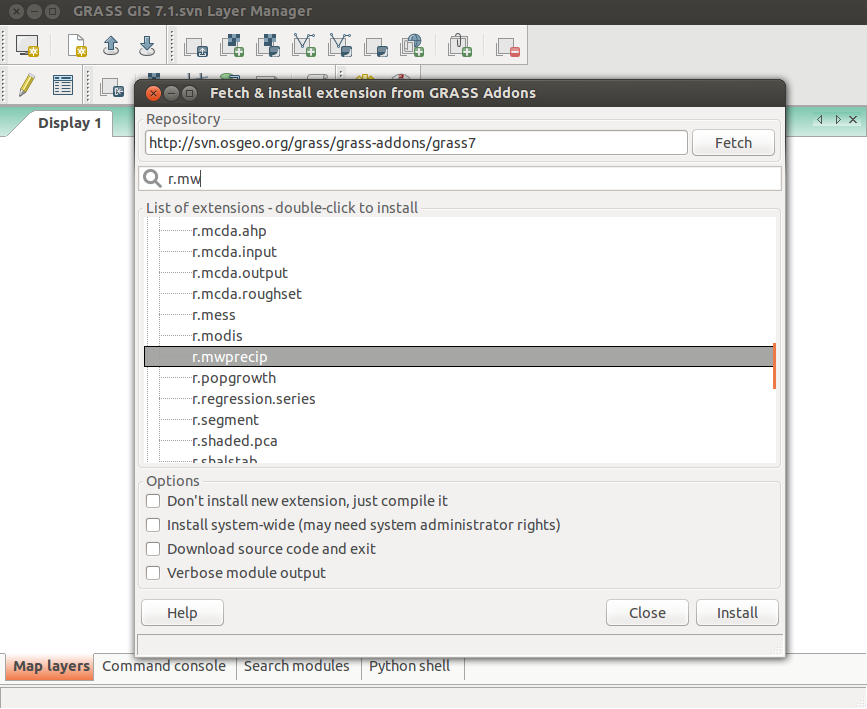
\includegraphics[width=0.6\textwidth]{./img/priloha/addons.png}
    \caption[DB]{Snímek okna modulu znázorňující volbu databáze   \centering  }
 \end{figure}


\subsection{Z příkazové řádky GRASS}

%Ke stahování modulů z externích Subversion repozitářů slouží modul \textit{g.extension}.

Stažení  modulu \textit{r.mwprecip} a \textit{v.link.precip} je možno pomocí spuštění \textit{g.extension} s následujícími parametry.
\begin{figure}[h!]
\begin{scriptsize}
\lstset{extendedchars=false,
escapeinside=''}
\begin{lstlisting}[style=mybash]
# Instalace modul'ů'
g.extension extension=r.mwprecip 
g.extension extension=v.link.precip     
# Spu'š'ten'í' modul'ů'
r.mwprecip
v.link.precip                                 
\end{lstlisting}
\end{scriptsize} 
\end{figure} 
\vskip-2ex

%\newpage
\section{Ukázka konfigurace parametrů modulu}
\label{appendix:ukazkakonf}
Pro názornost vytvořme následující zadání:
Data jsou uložena v databázi \textit{letnany}. Cílem zadání je vytvořit \textbf{rastry plošných interpolací} v časovém kroku 1 minuta. Tyto rastry nás zajímají pouze z \textbf{časového intervalu} od 2013-09-08 23:59:00 do 2013-09-09 23:59:00. Ze stejného období pro následující časoprostorové analýzy potřebujeme vytvořit \uv{časová okna} z časových řad srážkoměrů. Pro výpočet baseline známe  časové intervaly nulových srážek (suchá období). Z těchto suchých období chceme určit baseline z horního 96 \% \textbf{kvantilu} daných hodnot. Máme informaci o \textbf{rozbitých spojích} linkid= 63, 58 a 71. Jejich hodnoty pro odhady plošných srážek chceme ignorovat. K plošným interpolacím využijeme metody IDW s exponentem 1.6 a počtem bodů zasahujícím do výpočtu 35. Vizualizaci rastru nastavíme vlastní \textbf{tabulkou barev}. Pro interpolaci chceme linie nahradit  \textbf{rovnoměrně dvěma body}. Celý výpočet uložíme do \textbf{pracovního schematu} \textit{ukazka}.


\begin{figure}[h!]
\begin{scriptsize}
\lstset{extendedchars=false,
escapeinside=''}
\begin{lstlisting}[style=mybash]
#nastaven'í' p'ř''í'stupu k datab'á'zi.
database=letnany                          
\end{lstlisting}
\end{scriptsize} 
\end{figure} 
\vskip-2ex
\begin{figure}[h!]
    \centering
    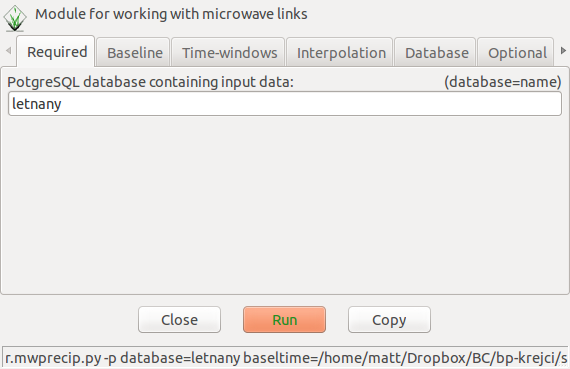
\includegraphics[width=0.5\textwidth]{./img/priloha/db.png}
    \caption[DB]{Okno modulu pro povinnou konfiguraci   \centering  }
 \end{figure}



 
\begin{figure}[h!]
\begin{scriptsize}
\lstset{extendedchars=false,
escapeinside=''}
\begin{lstlisting}[style=mybash]
#volba kvantilu a such'é'ho obdob'í' - v'ý'po'č'et baseline
statfce=quantile  quantile96 baseltime= adresa/k/souboru        
\end{lstlisting}
\end{scriptsize} 
\end{figure} 
\vskip-2ex

\begin{figure}[h!]
    \centering
    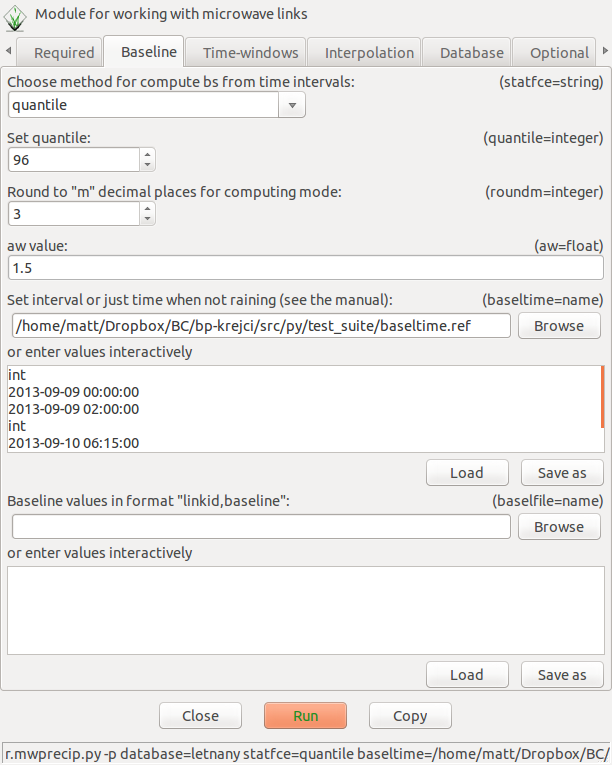
\includegraphics[width=0.5\textwidth]{./img/priloha/bs.png}
    \caption[TW]{Okno modulu pro konfiguraci určení baseline  \centering  }
 \end{figure}



\begin{figure}[h!]
\begin{scriptsize}
\lstset{extendedchars=false,
escapeinside=''}
\begin{lstlisting}[style=mybash]
#konfigurace časov'ý'ch oken pro interpolovan'é' rastry a sr'á''ž'kom'ě'ry
fromtime= 2013-09-08 23:59:00 totime= 2013-09-09 23:59:00\
lignore=cesta/ignorovanespoje v rgauges=cesta/k/slo'ž'ce
\end{lstlisting}
\end{scriptsize} 
\end{figure} 
\vskip-2ex
\begin{figure}[h!]
    \centering
    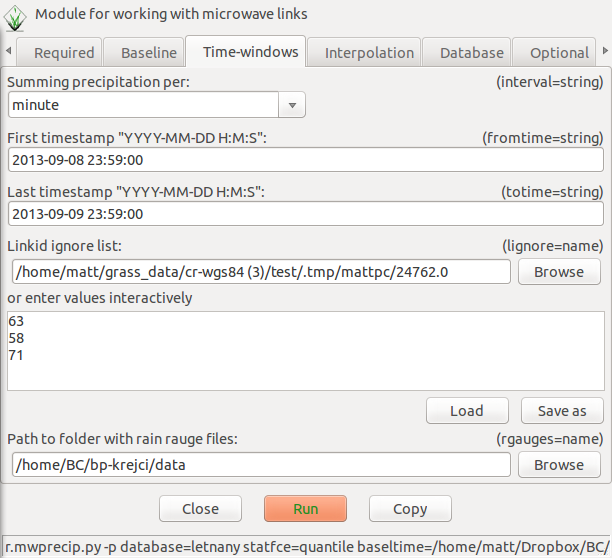
\includegraphics[width=0.5\textwidth]{./img/priloha/tw.png}
    \caption[TW]{Okno modulu pro konfiguraci vytvoření časových oken  \centering  }
 \end{figure}


\begin{figure}[h!]
\begin{scriptsize}
\lstset{extendedchars=false,
escapeinside=''}
\begin{lstlisting}[style=mybash]
#konfigurace plo'š'n'ý'ch interpolac'í'
isettings=grass.run_command( "v.surf.idw", input=points_nat, \
	column=attribute_col, output=out, npoints=35, power=1.8 )
pmethod=count step=2 color=cesta/k/tabulce/barevRGB \	   
-g 
\end{lstlisting}
\end{scriptsize} 
\end{figure} 
\vskip-2ex
\begin{figure}[h!]
    \centering
    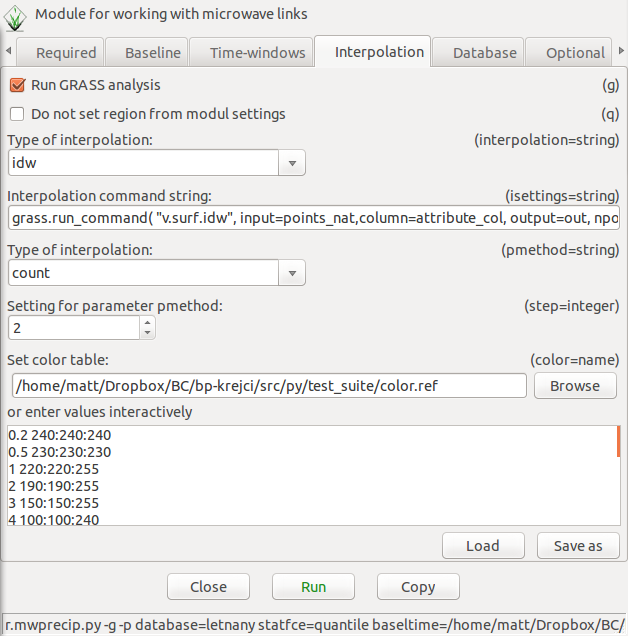
\includegraphics[width=0.5\textwidth]{./img/priloha/int.png}
    \caption[Interpolace]{Okno modulu pro  konfiguraci plošných interpolací  \centering  }
 \end{figure}

\begin{figure}[h!]
\begin{scriptsize}
\lstset{extendedchars=false,
escapeinside=''}
\begin{lstlisting}[style=mybash]
#pojmenov'á'n'í' pracovn'í'ho sch'é'ma
schema=ukazka
\end{lstlisting}
\end{scriptsize} 
\end{figure} 
\vskip-2ex
\begin{figure}[h!]
    \centering
    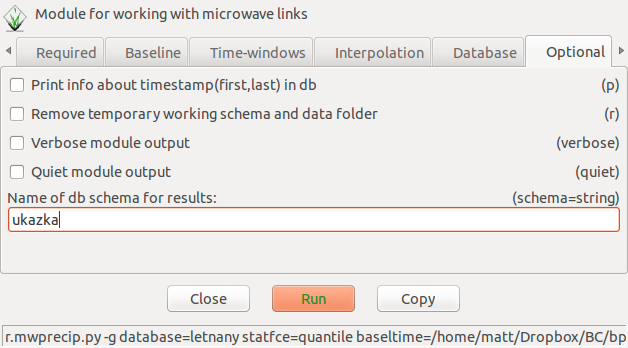
\includegraphics[width=0.5\textwidth]{./img/priloha/opt.png}
    \caption[Optional]{Okno pro nastavení pracovního schéma a doplňkových parametrů \centering  }
 \end{figure}





\end{document}









